% =========================================================================
% SECTION 5.1: interleaved boost converter simulation
% =========================================================================

\section{Central and String Interleaved Boost with Load (High Ratings)}

\subsection{Introduction}
In the field of modern electrical engineering, the transition from theoretical mathematical equations to tangible physical hardware represents one of the most critical and challenging phases of a graduation project. Designing advanced power electronics, control algorithms, and renewable energy systems involves managing highly non-linear dynamics, transient phenomena, and delicate hardware components. In a practical laboratory setting, executing direct "trial-and-error" testing on real hardware is not only financially prohibitive but also poses significant safety risks, as minor controller errors can lead to catastrophic component failures. Therefore, engineering design requires a reliable and intermediate validation phase to guarantee system safety and performance before hardware implementation.

To bridge this gap between theory and hardware,simulation has become an indispensable tool in engineering research and education. Simulation software allows us to build precise mathematical twins of physical components—such as photovoltaic arrays, switching converters, and closed-loop controllers—and observe their behavioral dynamics under safely controlled conditions. It provides the unique capability to test worst-case operational scenarios, analyze transient responses, and fine-tune controller coefficients without the risk of damaging expensive laboratory equipment.

For this project, MATLAB and Simulink were selected as the primary simulation ecosystem. MATLAB’s powerful numerical computing engine, combined with Simulink’s specialized Simscape Electrical libraries, allows for the seamless integration of physical power hardware with complex control logic. From executing high-speed Pulse Width Modulation (PWM) to designing multi-state Global Maximum Power Point Tracking (GMPPT) algorithms, MATLAB enables us to thoroughly debug code, verify system stability, and optimize electrical performance. Ultimately, the simulation framework developed in this work serves as the foundational blueprint, providing the rigorous analytical validation necessary to transition our designs into a successful, real-world engineering reality.
\newpage

\subsection{PV array distribution}

\subsubsection{Power calculation}
If per day energy needed = 42.5 KW.h, so the power needed from PV array = 8500W (regarding that the sun remains at its peak intensity for five hours).

This PV specification meets the requirements:
\begin{figure}[H]
    \centering
    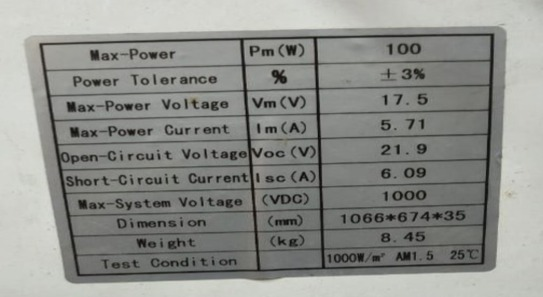
\includegraphics[width=0.75\textwidth]{Figures/PV1.jpg}
    \caption{PV specification.}
    \label{fig:PV specification}
\end{figure}
\begin{equation}
    P_{\text{module}} = V_m \times I_m = 40.9\,\text{V} \times 17.36\,\text{A} = 710\,\text{W}
\end{equation}
\begin{equation}
    \text{Number of modules} = \frac{8500\,\text{W}}{710\,\text{W}} \approx 12\text{ Panels}
\end{equation}
\subsubsection{PV configuration}
The photovoltaic system simulation is initiated by defining the standard environmental parameters. As shown in Figure 5.2, the PV array block receives two primary environmental inputs: a constant solar irradiance (Ir) of 1000 W/m2 and a cell temperature (T) of 25°C, representing Standard Test Conditions (STC).
Connected across the output terminals of the PV block is an anti-parallel diode acting as a bypass protection layer against partial shading conditions and potential hot-spot development. To stabilize the DC bus voltage and mitigate high-frequency transient ripple resulting from downstream switching operations, an RC network consisting of a series resistor and a parallel capacitor is integrated at the PV output interface.
\begin{figure}[H]
    \centering
    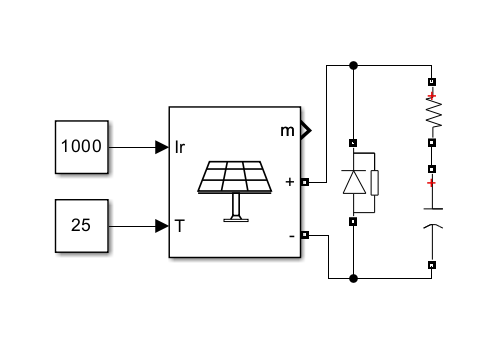
\includegraphics[width=0.75\textwidth]{Figures/PV configuration.png}
    \caption{PV configuration.}
    \label{fig:PV configuration}
\end{figure}
\begin{figure}[H]
    \centering
    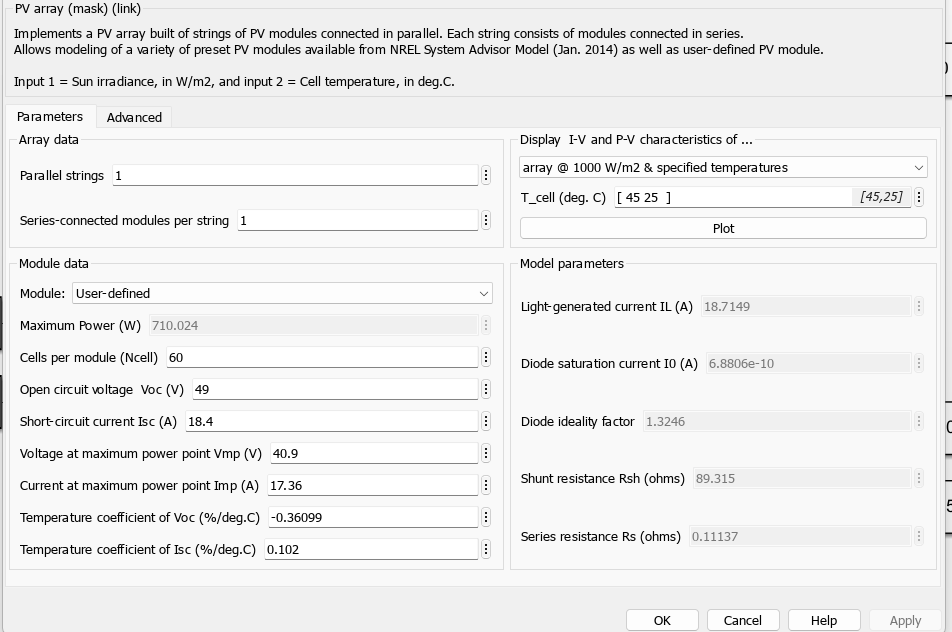
\includegraphics[width=1\textwidth]{Figures/spec.png}
    \caption{PV block specifications.}
    \label{fig:PV block specifications}
\end{figure}

\newpage
\subsubsection{Array configuration}
The general rules for array sizing are:
\begin{itemize}
  \item $N_s$ (number of modules in series) increases array voltage:
        $V_{\text{array}} = N_s \times V_{\text{module}}$
  \item $N_p$ (number of parallel strings) increases array current:
        $I_{\text{array}} = N_p \times I_{\text{module}}$
\end{itemize}
 \begin{table}[htbp]
    \centering
    \caption {Different ways to distribute these twelve modules:}
    \label{tab:pv_configurations}
    \small
    \begin{tabular}{|c|c|c|c|}
        \hline
        \textbf{Configuration ($N_s \times N_p$)} & \textbf{Voltage ($V$)} & \textbf{Current ($I$)} & \textbf{Power ($W$)} \\ \hline
        1 * 12 & 490.8 & 17.36  & 8520 \\ \hline
        2 * 6  & 245.4 & 34.72  & 8520 \\ \hline
        3 * 4  & 163.6 & 52.08  & 8520 \\ \hline
        4 * 3  & 122.7 & 69.44  & 8520 \\ \hline
        6 * 2  & 81.8  & 104.16 & 8520 \\ \hline
        12 * 1 & 40.9  & 208.32 & 8520 \\ \hline
    \end{tabular}
\end{table}
Configuration 1 or Configuration 2 are the best choices. They keep the voltage high enough to match the input DC-link requirements of standard inverters while keeping current low, which minimizes power losses across the transmission cables.
To show the difference between central and string configurations, configuration 2 will be used in simulation.
\subsection{Central Configuration with Load}
In this configuration, a number of series PV arrays are connected in a central manner, which means the positive terminal of each string are connected and the negative terminals are also connected.
In central configuration only one boost converter is used to step up the voltage for the whole system from 245.4V to 600V as the battery of EV is 400V so the dc link voltage must be more than 400V.
\begin{figure}[H]
    \centering
    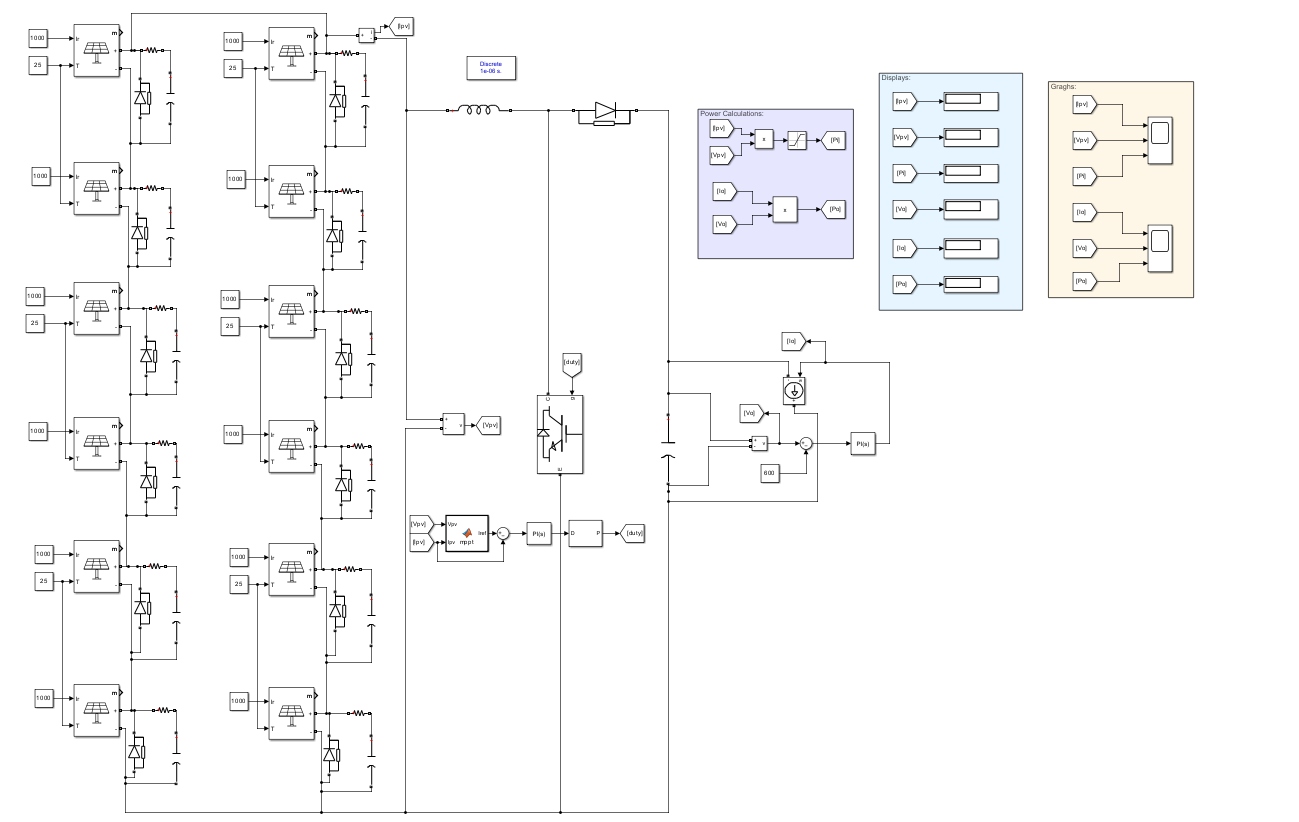
\includegraphics[width=1\textwidth]{Figures/central1.png}
    \caption{Central array configuration.}
    \label{fig:central array configuration.}
\end{figure}
\subsubsection{Boost Converter}
Boost converter is used to boost the input voltage from 245.4V (40.9*6) to 600V that will be used in the DC link to charge Electric Vehicles.
Calculations can be shown as follows:
\begin{align}
  D &= 1 - \frac{V_{\text{in}}}{V_{\text{out}}} = 1 - \frac{245.4}{600} = 0.591 \\[4pt]
  f_s &= \SI{10}{\kilo\hertz} \\[4pt]
  R &= \frac{V_{\text{out}}}{I_{\text{out}}} = \frac{600}{13.9} = \SI{43.165}{\ohm} \\[4pt]
  L_{\min} &= \frac{R \cdot D \cdot (1-D)^2}{2\,f_s}
             = \frac{43.165 \times 0.591 \times (0.409)^2}{2 \times 10000}
             \approx \SI{0.213}{\milli\henry} \\[4pt]
  \Delta I_L &= \frac{V_{\text{in}} \cdot D}{L \cdot f_s}
              = \frac{245.4 \times 0.591}{0.015 \times 10000}
              \approx \SI{0.967}{\ampere}
\end{align}

A practical inductance of $L = \SI{15}{\milli\henry}$ is chosen, well above $L_{\min}$, to ensure
continuous conduction mode (CCM) with a comfortable margin.

\medskip
\newpage
\noindent\textbf{Output Capacitor (DC-link):} A bulk capacitor of $C = \SI{50e-3}{\farad}$
is selected because:
\begin{itemize}
  \item It filters high-frequency switching noise to provide a stable, constant \textbf{600\,V} DC output.
  \item It stores energy to support the system during sudden changes in solar power or load demand.
  \item It minimises voltage ripple, ensuring the power delivered to the next stage is clean and steady.
\end{itemize}

\subsubsection{MPPT Implementation}
\begin{figure}[H]
    \centering
    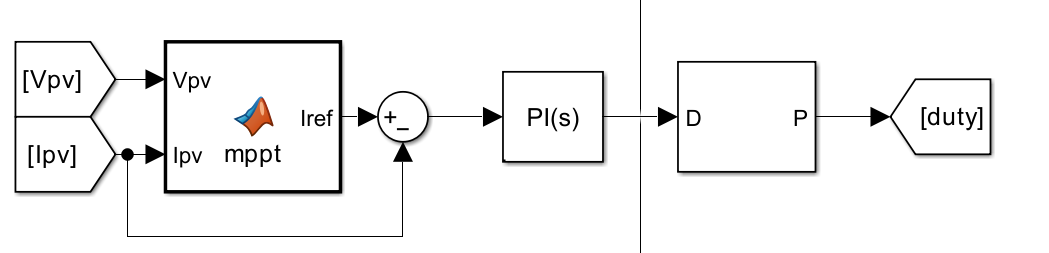
\includegraphics[width=1\textwidth]{Figures/mppt.png}
    \caption{MPPT Implementation.}
    \label{fig:MPPT Implementation.}
\end{figure}
\paragraph{Stage 1 — Current Reference Generation}
\begin{itemize}
  \item The MPPT function takes two inputs $V_{pv}$ (panel voltage) and $I_{pv}$ (panel
        current) and outputs $I_{\text{ref}}$, the reference current that controls how
        much power is drawn from the panel.
  \item The actual measured current is subtracted from $I_{\text{ref}}$ to produce an
        error signal. A continuous-time PI controller ($K_p = 0.05$, $K_i = 10$)
        processes this error to eliminate steady-state offset and smooth the response.
        Because the PI output is in amperes, and the DC-DC converter operates only on a
        duty cycle (a dimensionless number between 0 and 1), a further conversion stage
        is required.
\end{itemize}

\paragraph{Stage 2 — Duty Cycle Generation}
\begin{itemize}
  \item \textbf{D (divider):} Normalises the PI output by dividing by $V_{pv}$. From
        the boost-converter inductor ripple equation,
        $\Delta I_L = V_{\text{in}}\,D\,/\,(L\,f_s)$, the same duty cycle produces
        different currents at different input voltages. Dividing by $V_{pv}$ removes
        this dependency so the control loop behaves identically across the full
        operating voltage range.
  \item \textbf{P (gain block):} Scales the small dimensionless result into the $[0,1]$
        range expected by the PWM generator.
  \item The final output is the duty cycle signal sent to the boost converter switch.
\end{itemize}
\newpage
\paragraph{How the code works}
\begin{lstlisting}[language=Matlab, caption={MATLAB code implementing the FSM-based global MPPT control loop.}]
function Iref = mppt(Vpv, Ipv)
    persistent V_target Pmax Vbest mode timer;
    
    Ts = 1e-6;
    
    % Voltage sweep parameters - sweep Vpv from high to low
    V_oc_est = 280;           % Estimated open circuit voltage
    V_scan_min = 240;         % Minimum scan voltage
    V_ramp_rate = 150;        % V/s sweep rate
    
    if isempty(V_target)
        V_target = V_oc_est;
        Pmax = 0;
        Vbest = 240;          % Start with nominal MPP voltage
        mode = 0;
        timer = 0;
    end
    
    Ppv = Vpv * Ipv;
    
    switch mode
        case 0  % RESET - go to high voltage (low current)
            V_target = V_oc_est;
            Pmax = 0;
            if Vpv > 270       % Near Voc
                mode = 1;
            end
            
        case 1  % SCAN - sweep voltage DOWN to find global Pmax
            % Record power at each voltage
            if Ppv > Pmax
                Pmax = Ppv;
                Vbest = V_target;
            end
            
            V_target = V_target - (V_ramp_rate * Ts);
            
            if V_target <= V_scan_min
                mode = 2;
            end
            
        case 2  % RETURN to Vbest
            if V_target < Vbest
                V_target = V_target + (300 * Ts);
            else
                V_target = Vbest;
                mode = 3;
                timer = 0;
            end
            
        case 3  % HOLD
            timer = timer + Ts;
            if timer >= 5
                mode = 0;
            end
    end
    
    % INNER LOOP: Current controller to regulate Vpv to V_target
    % Simple P-control: if Vpv > V_target, increase current (load more)
    %                  if Vpv < V_target, decrease current (load less)
    persistent err_int;
    if isempty(err_int), err_int = 0; end
    
    err = Vpv - V_target;           % Positive = need more load
    err_int = err_int + err * Ts;
    err_int = max(min(err_int, 50), -50);  % Anti-windup
    
    Kp = 1;   % Proportional gain
    Ki = 200;   % Integral gain
    
    % Base current + correction
    I_calc = 20 + Kp * err + Ki * err_int;
    
    % Limit output
    Iref = max(min(I_calc, 35), 0);
end
\end{lstlisting}

\medskip
\noindent\textbf{Code Operation Breakdown:}
\begin{itemize}
    \item \textbf{Lines 2--10:} Initialize persistent tracking metrics and operational variables. These memory boundaries ensure tracking parameters are preserved across discrete high-speed execution frames ($T_s = 1\ \mu\text{s}$). A voltage ramp rate of $V_{\text{ramp\_rate}} = 150\text{ V/s}$ combined with a sample time of $T_s = 1\ \mu\text{s}$ means that the target voltage drops by exactly $150 \times 10^{-6} = 0.00015\text{ V}$ per execution step. This configuration results in an extremely fine-grained sweep profile that prevents the tracking algorithm from missing narrow global power peaks.
    
    \item \textbf{Lines 11--17:} Execute the baseline cold-start routine exactly once at simulation startup. This block sets the initial target voltage near the open-circuit threshold, resets the captured power registers to zero, and forces a direct transition into the tracking loop.
    \newpage
    \item \textbf{Lines 21--27:} Mode 0 (Reset Routine): The algorithm establishes a high boundary threshold target voltage ($V_{\text{target}} = 270\text{ V}$) where the converter circuit draws approximately zero current from the source terminals.Once the measured PV array voltage stabilizes and settles within proximity of this open-circuit reference point, the sequential sweep routine is automatically triggered.
    
    \item \textbf{Lines 29--40:} Mode 1 (Global Scan Phase): The algorithm dynamically forces the operational target voltage reference to decrease linearly across the predefined sweeping region. As the voltage is pulled down, the controller evaluates the instantaneous power extraction profile ($P_{\text{pv}} = V_{\text{pv}} \times I_{\text{pv}}$). If the instantaneous computed power exceeds the highest previously logged power value ($P_{\text{max}}$), the internal registers overwrite the historical maximum with the updated peak value ($P_{\text{max}} = P_{\text{pv}}$) and log the exact voltage coordinate as the optimal reference ($V_{\text{best}} = V_{\text{pv}}$).
    
    \item \textbf{Lines 42--49:} Mode 2 (Peak Return Phase): The linear global scanning sweep terminates automatically once the target tracking voltage descends to its lower operational bound ($240\text{ V}$). Upon reaching this threshold, the state machine shifts execution modes and systematically ramps the reference voltage back upward until it perfectly aligns with the captured optimal tracking coordinate ($V_{\text{best}}$).
    
    \item \textbf{Lines 51--56:} Mode 3 (Maximum Power Point Hold): The controller latches onto $V_{\text{best}}$ and holds this steady profile for a fixed duration of $5\text{ s}$ to maximize steady-state energy extraction without hunting oscillations. When the tracking timer expires, the block loops back to Mode 0 to re-evaluate the global P-V curve for updated atmospheric or partial shading alterations.
    
    \item \textbf{Lines 58--76:} Closed-Loop Reference Control Tracking: A continuous Proportional - Integral (PI) feedback loop ensures the actual physical panel voltage ($V_{\text{pv}}$) remains dynamically locked onto the tracking reference command ($V_{\text{target}}$) by actively adjusting the current reference output ($I_{\text{ref}}$):
    \begin{itemize}
        \item \textbf{Case A ($V_{\text{pv}} > V_{\text{target}}$):} The resulting error signal evaluates as positive. The loop increases the output current reference ($I_{\text{ref}}$) to draw more power from the PV array, which unloads the voltage down toward the target.
        \item \textbf{Case B ($V_{\text{pv}} < V_{\text{target}}$):} The error evaluates as negative. The controller decreases $I_{\text{ref}}$ to unload the array, allowing the internal cell capacitance to charge up toward the desired command.
    \end{itemize}
    To counter integrator windup and prevent mathematical saturation under transient changes, an anti-windup clamping threshold ($\pm 50$) is applied directly to the integration accumulator, while the reference output current command ($I_{\text{ref}}$) is strictly capped between $0\text{ A}$ and $35\text{ A}$ to protect downstream hardware components from overcurrent damage.
\end{itemize}
\newpage
\subsubsection{DC Link Voltage}
The control system ensures the output voltage remains constant at 600V by employing a feedback loop that compares the measured DC-link voltage with a 600V reference signal. The resulting error is processed by a PI Controller, which generates the necessary power or current commands to balance the energy flow. This regulation is vital to stabilize the DC bus against fluctuations in solar irradiance and load variations, ensuring the system operates at its designed 8520W peak power efficiently.

\subsubsection{Results of Simulation in Case of No Shading}
\noindent
\begin{minipage}[t]{0.5\textwidth}
\vspace{0pt}
\begin{itemize}
  \item As shown, current is almost $17.36 \times 2$, the input voltage is also aligned
        with design calculations and output power is 8419\,W, ideally should be 8520\,W,
        but there are switching losses and conduction losses (diodes have forward voltage,
        etc.).

  \item \textbf{DC-Link Stability:} The output voltage ($V_{DC}$) is maintained at
        exactly 600\,V. This proves that the DC-Link Voltage Control loop
        ($K_p = 3$, $K_i = 50$) and the Bulk Capacitor are effectively regulating the
        output despite the high-power flow.

  \item Ripples of inductor current $= 35.18 - 34.2 = 0.98$\,A.
\end{itemize}
\end{minipage}
\hfill
\begin{minipage}[t]{0.4\textwidth}
\vspace{0pt}
  \centering
  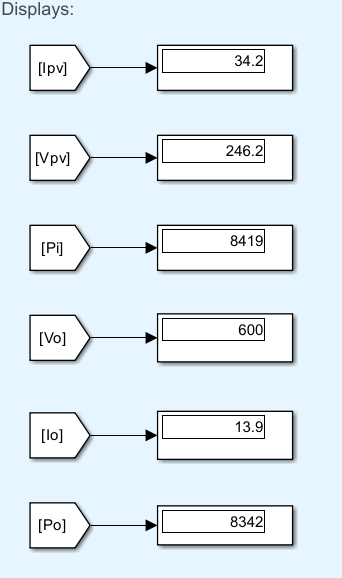
\includegraphics[width=\textwidth]{Figures/displaycentral1.png}
  \captionof{figure}{Displays of central configuration at no shading.}
  \label{fig:Displays of central configuration at no shading}
\end{minipage}
\paragraph{Graphs}
\begin{figure}[H]
    \centering
    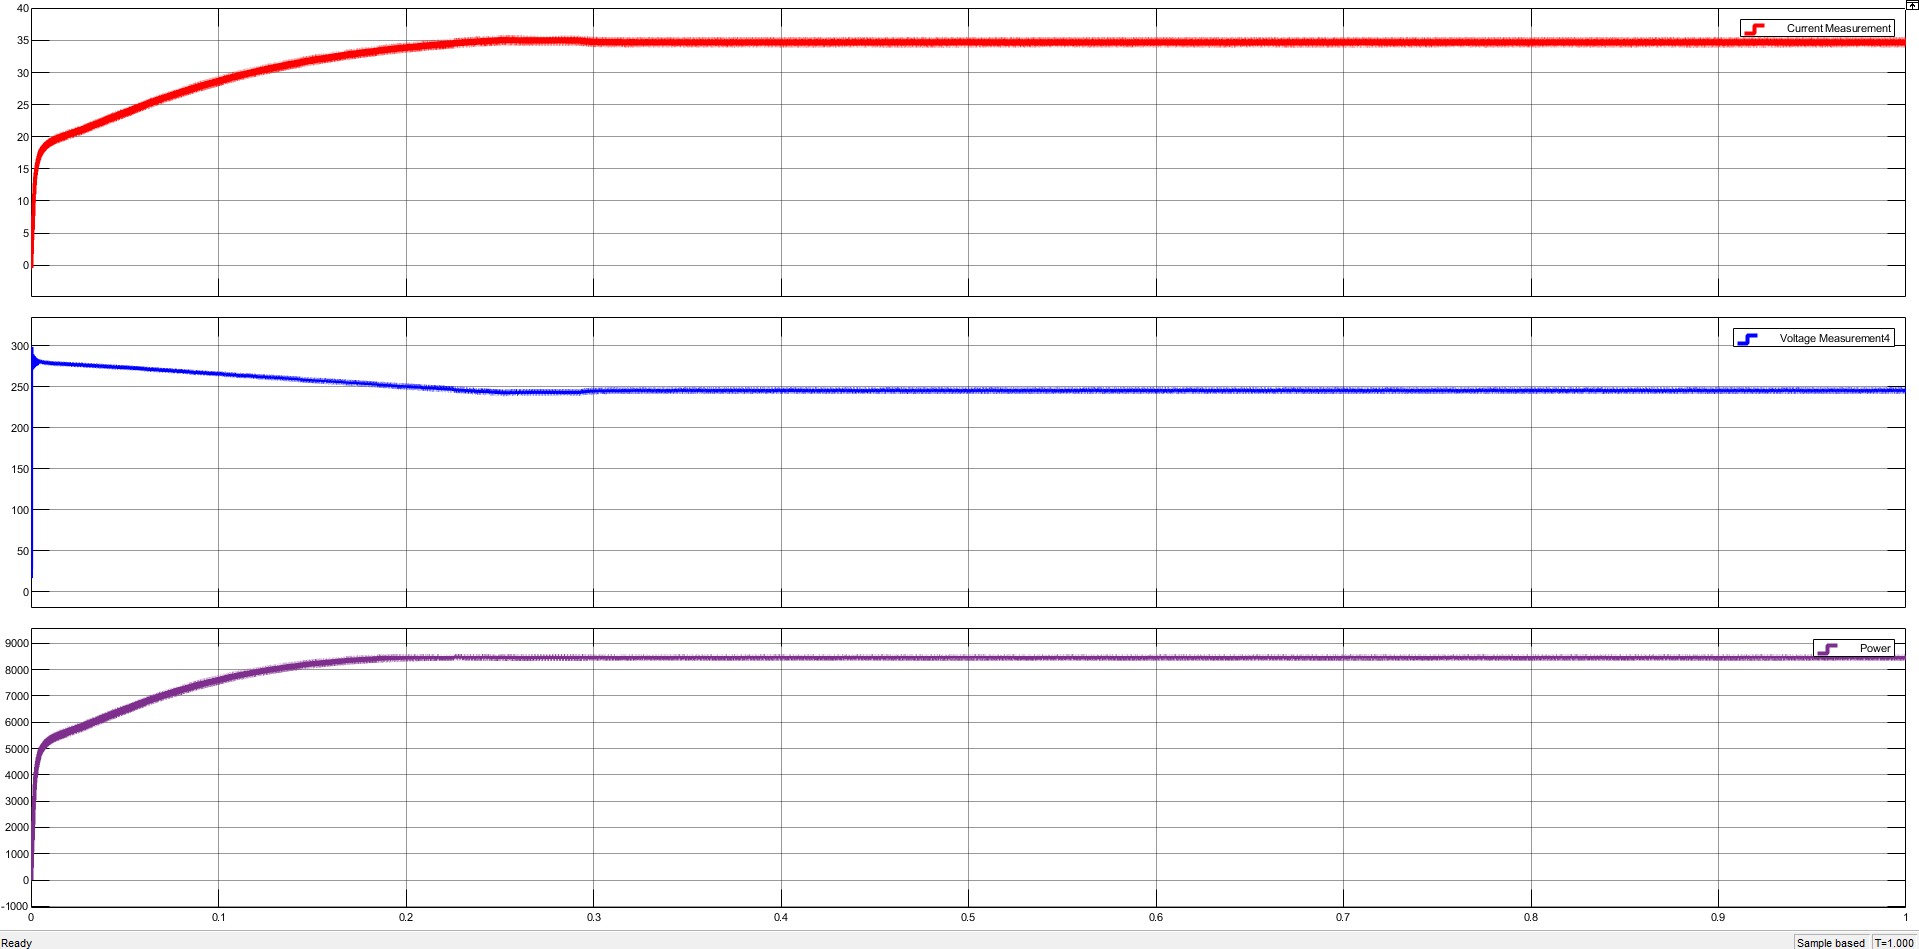
\includegraphics[width=1.1\textwidth]{Figures/5.1.7.png}
    \caption{Input current, voltage, power at no shading.}
    \label{fig:Input current, voltage, power at no shading}
\end{figure}
\begin{figure}[H]
    \centering
    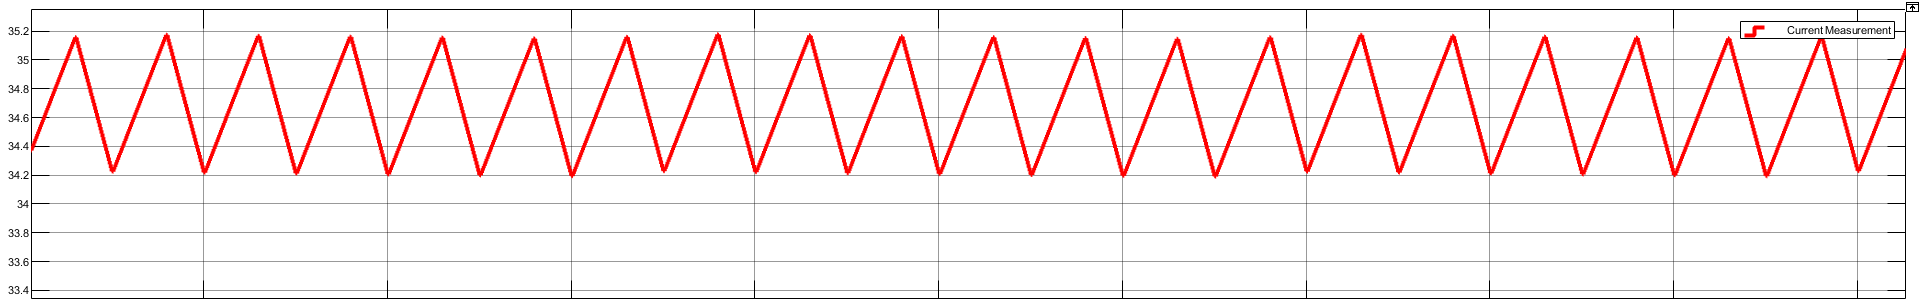
\includegraphics[width=1.1\textwidth]{Figures/5.1.8.png}
    \caption{Ripples of inductor current at no shading.}
    \label{fig:Ripples of inductor current at no shading}
\end{figure}
\begin{figure}[H]
    \centering
    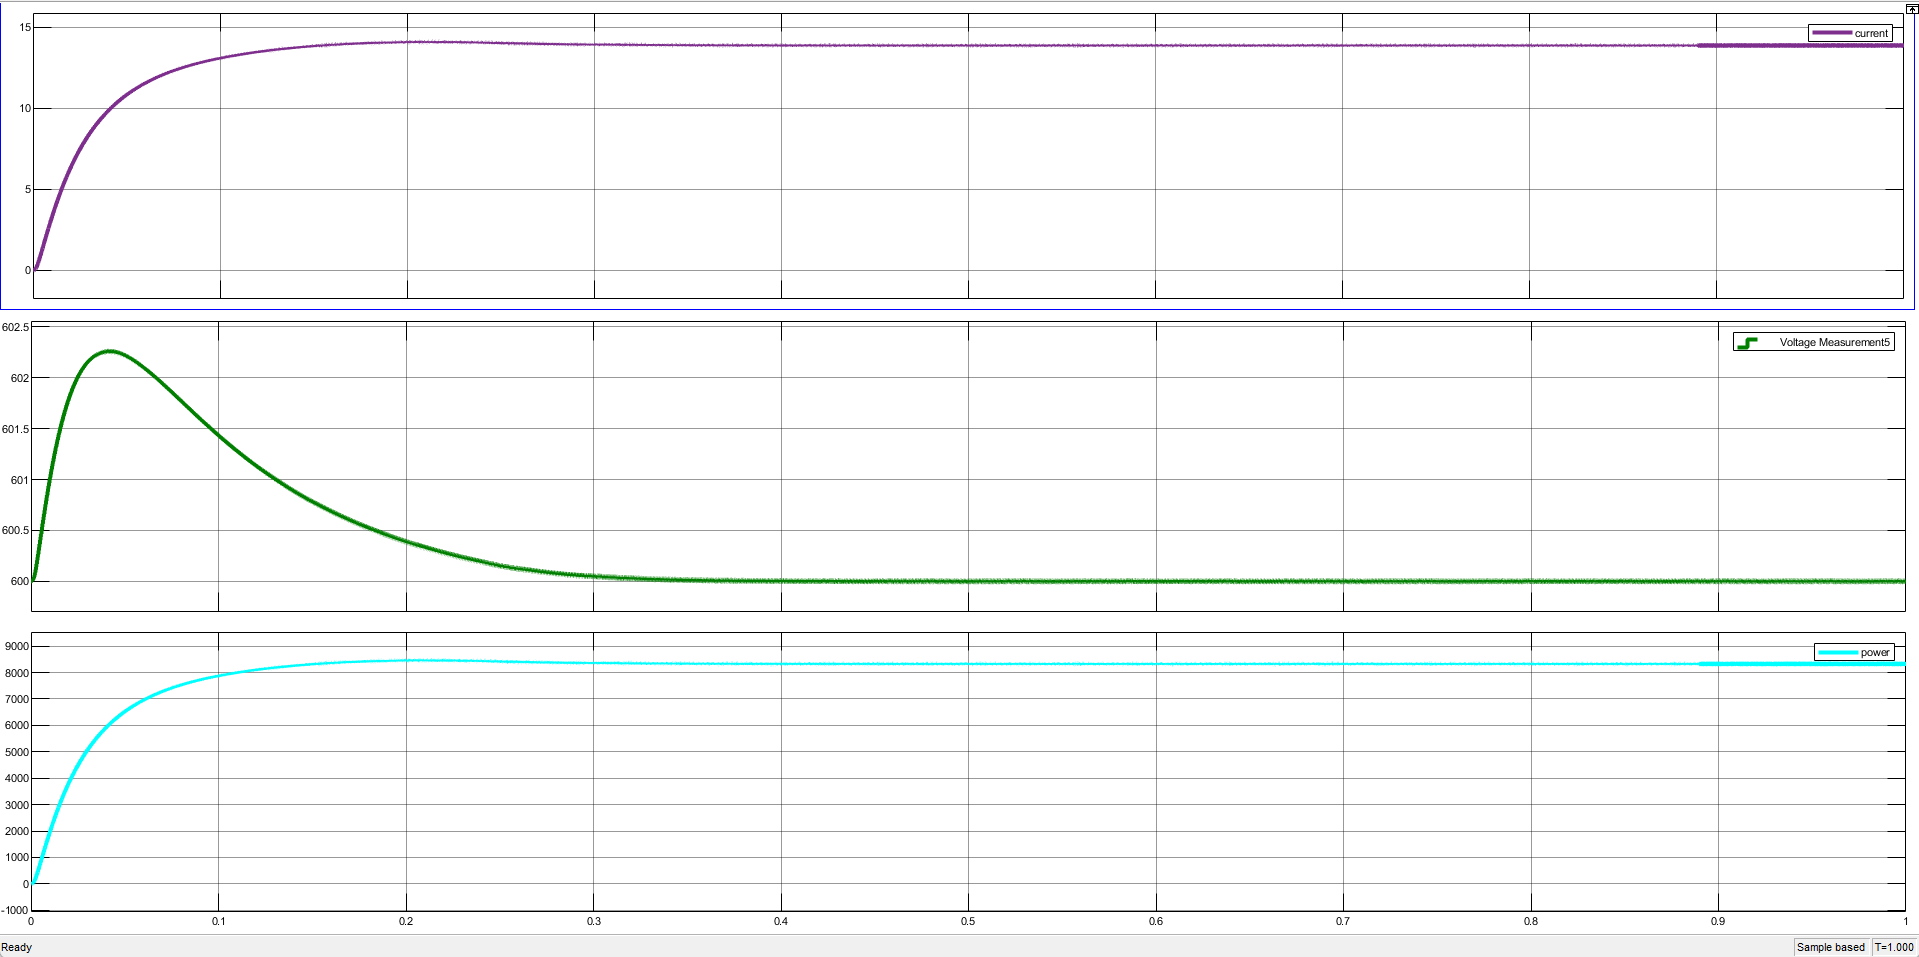
\includegraphics[width=1.1\textwidth]{Figures/5.1.9.png}
    \caption{Output current, voltage, power at no shading.}
    \label{fig:Output current, voltage, power at no shading}
\end{figure}

\subsubsection{Results of Simulation in Case of Shading (Ir = 800) at One Module}
\noindent
\begin{minipage}[t]{0.5\textwidth}
\vspace{0pt}
\begin{itemize}
  \item As shown, the output power decreases as the current decreases, but the Vpv is almost constant.
  \item Dc link voltage still maintained at 600\,V due to closed loop with PI.
  \item Ripples of inductor current $= 31.8 - 31 = 0.8$\,A.
\end{itemize}
\end{minipage}
\hfill
\begin{minipage}[t]{0.4\textwidth}
\vspace{0pt}
  \centering
  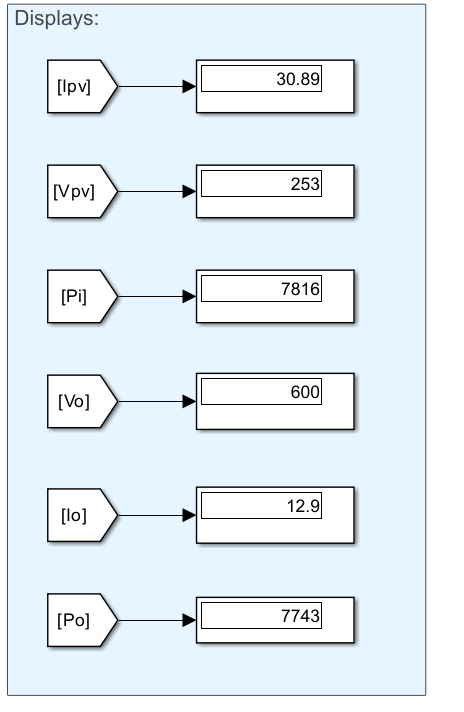
\includegraphics[width=\textwidth]{Figures/5.1.10.png}
  \captionof{figure}{Displays of central configuration at 800 shading.}
  \label{fig:Displays of central configuration at 800 shading}
\end{minipage}
\paragraph{Graphs}
\begin{figure}[H]
    \centering
    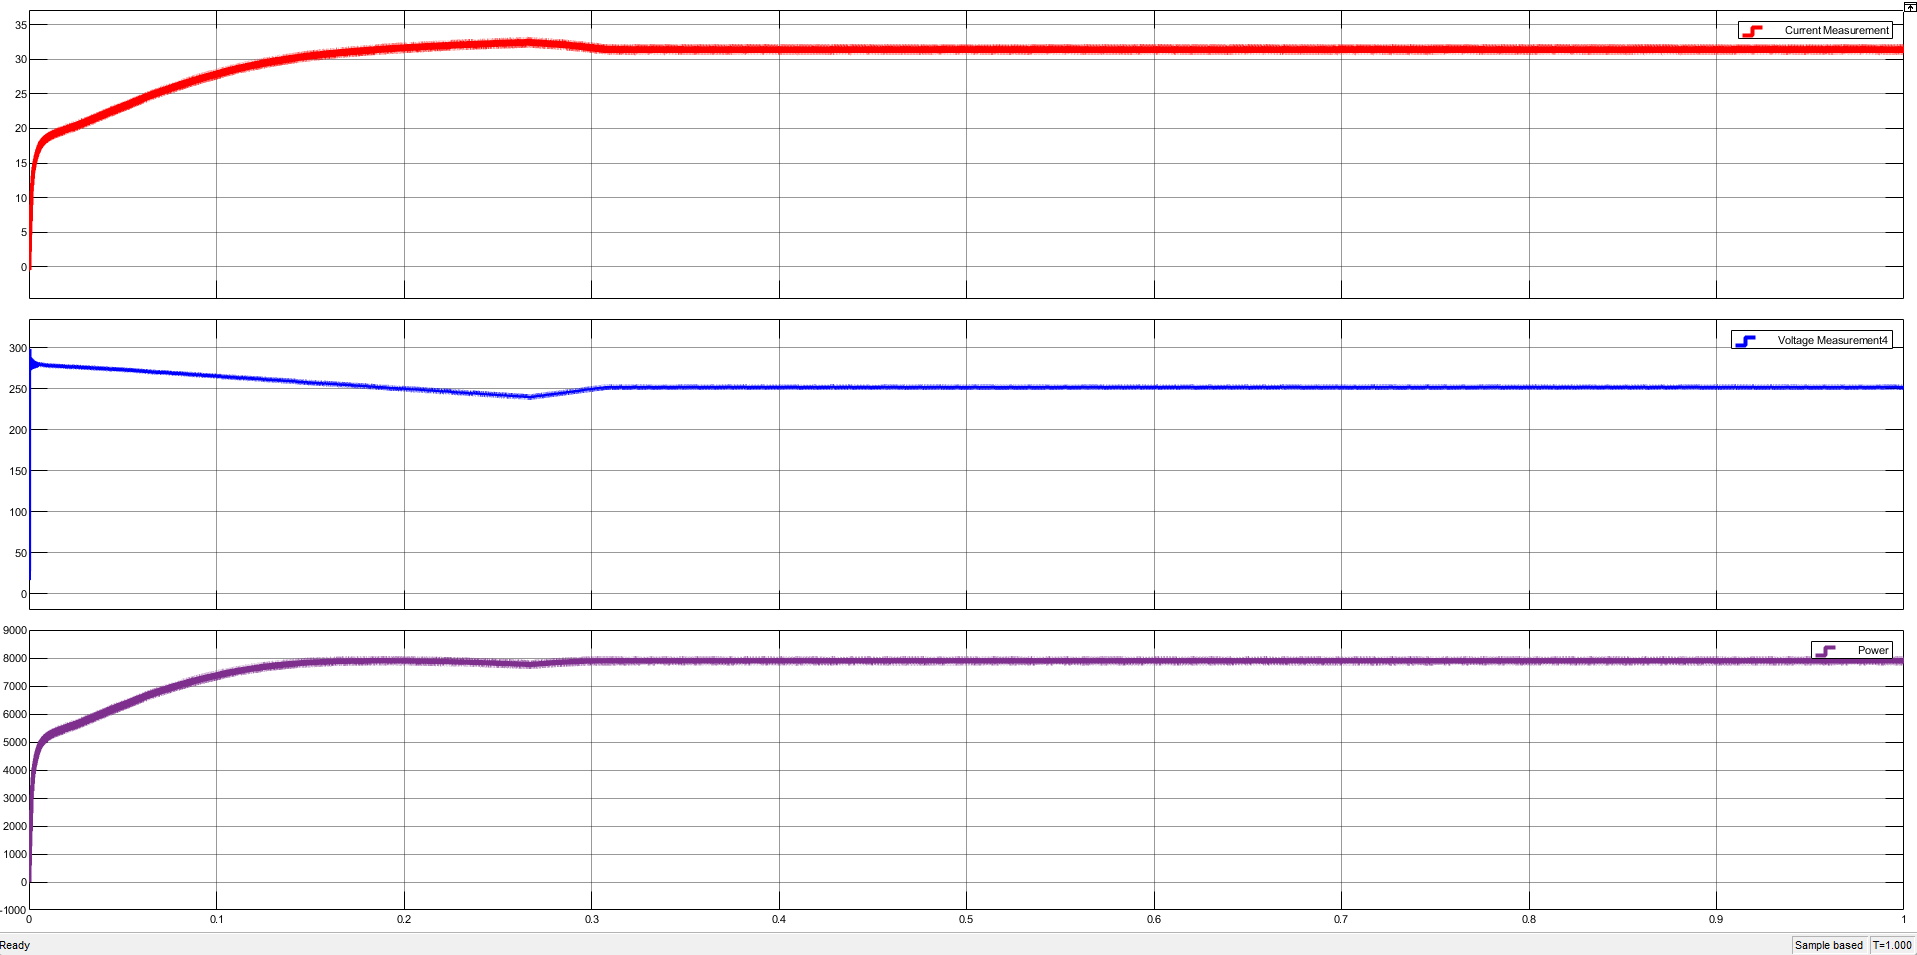
\includegraphics[width=1.1\textwidth]{Figures/5.1.11.png}
    \caption{Input current, voltage, power at 800 shading.}
    \label{fig:input current, voltage, power at 800 shading}
\end{figure}
\begin{figure}[H]
    \centering
    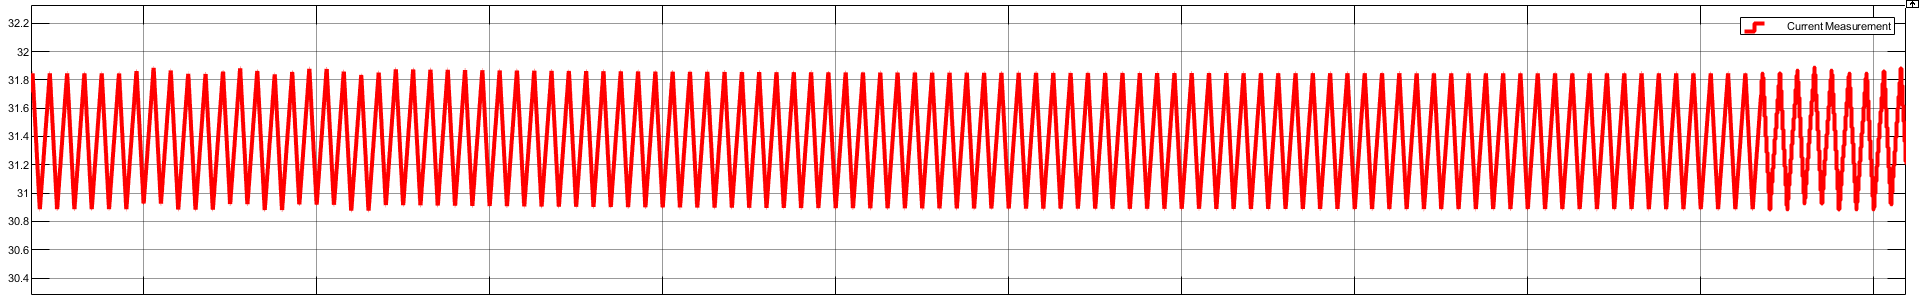
\includegraphics[width=1.1\textwidth]{Figures/5.1.12.png}
    \caption{Ripples of inductor current at 800 shading.}
    \label{fig:ripples of inductor current at 800 shading}
\end{figure}
\begin{figure}[H]
    \centering
    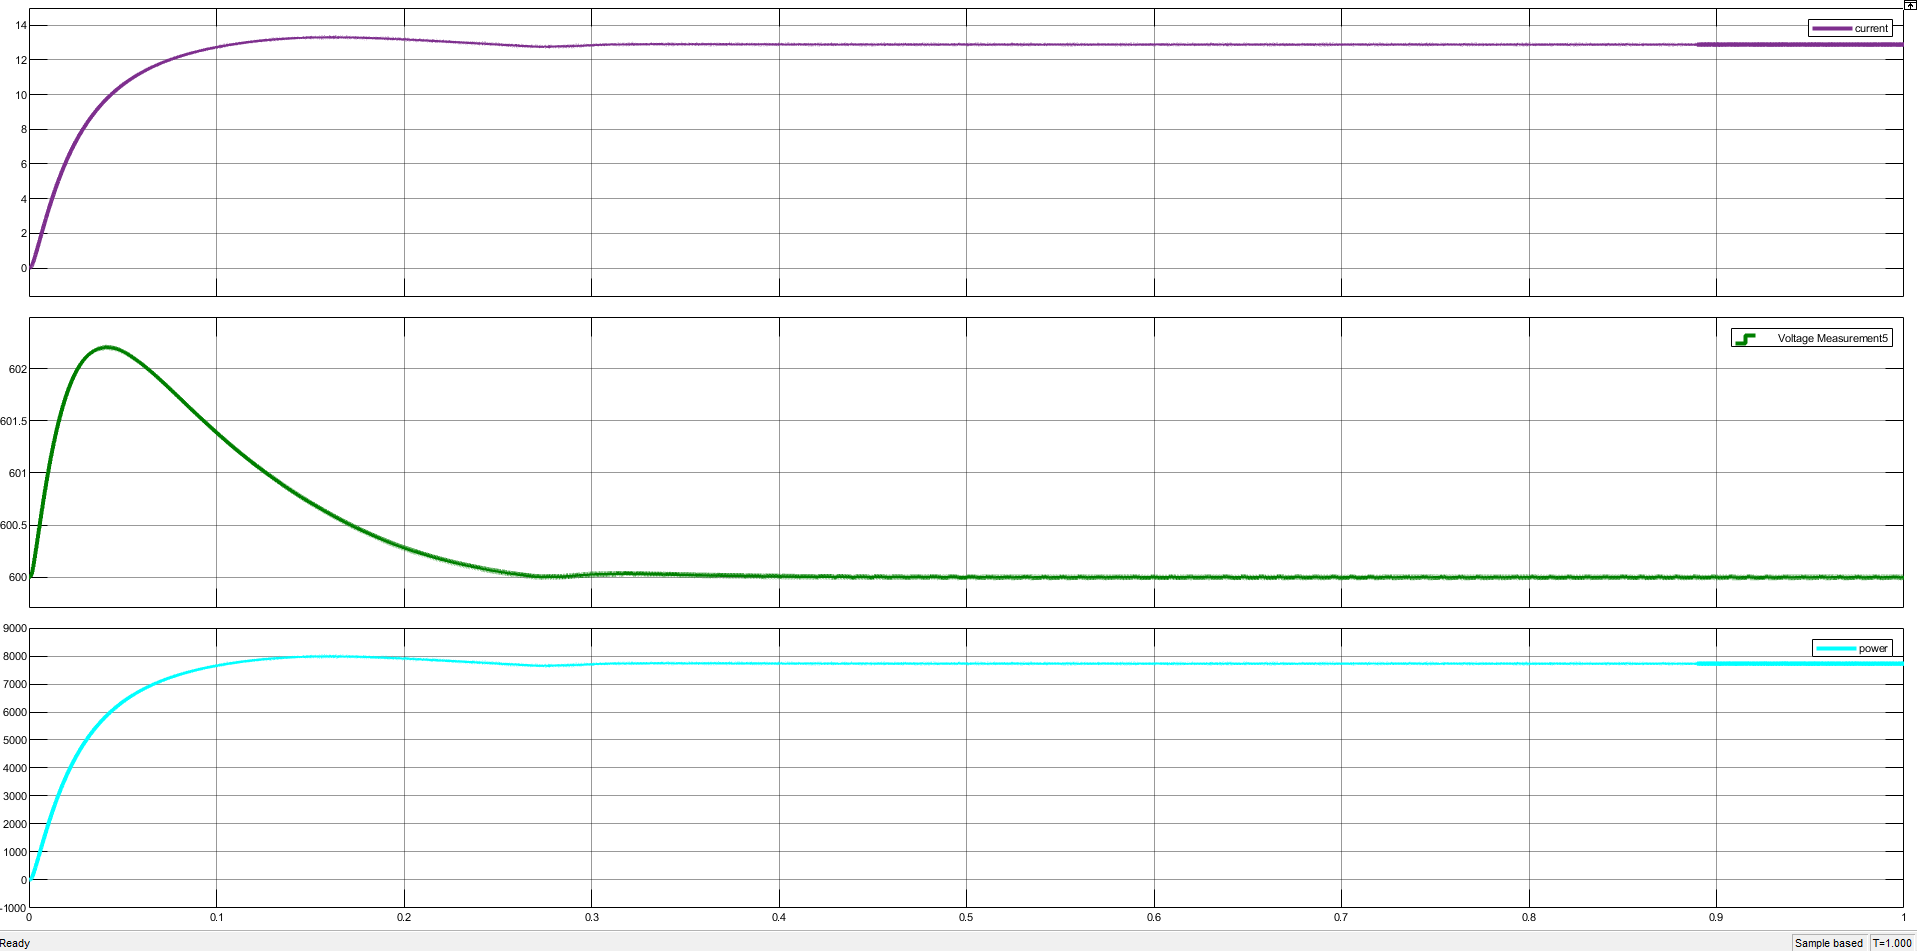
\includegraphics[width=1.1\textwidth]{Figures/5.1.13.png}
    \caption{Output current, voltage, power at 800 shading.}
    \label{fig:Output current, voltage, powerat 800 shading}
\end{figure}

\subsubsection{Results of Simulation in Case of Shading (Ir = 500) at One Module}
\noindent
\begin{minipage}[t]{0.5\textwidth}
\vspace{0pt}
\begin{itemize}
  \item As shown, the output power decreases much more as the current decreases more than the current in the pervious case as Ir decreases, but the Vpv is almost constant.
  \item Dc link voltage still maintained at 600V due to closed loop with PI.
  \item Ripples of inductor current $= 26.7 - 25.8 = 0.9$\,A.
\end{itemize}
\end{minipage}
\hfill
\begin{minipage}[t]{0.4\textwidth}
\vspace{0pt}
  \centering
  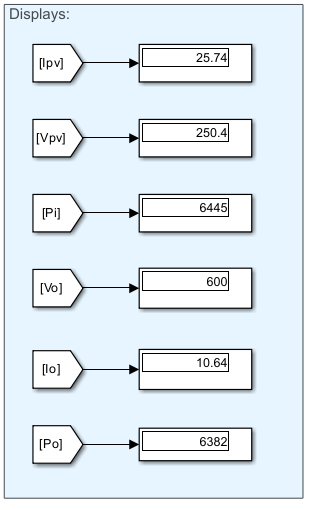
\includegraphics[width=\textwidth]{Figures/5.1.14.png}
  \captionof{figure}{Displays of central configuration at 500 shading.}
  \label{fig:Displays of central configuration at 500 shading}
\end{minipage}
\paragraph{Graphs}
\begin{figure}[H]

\centering
    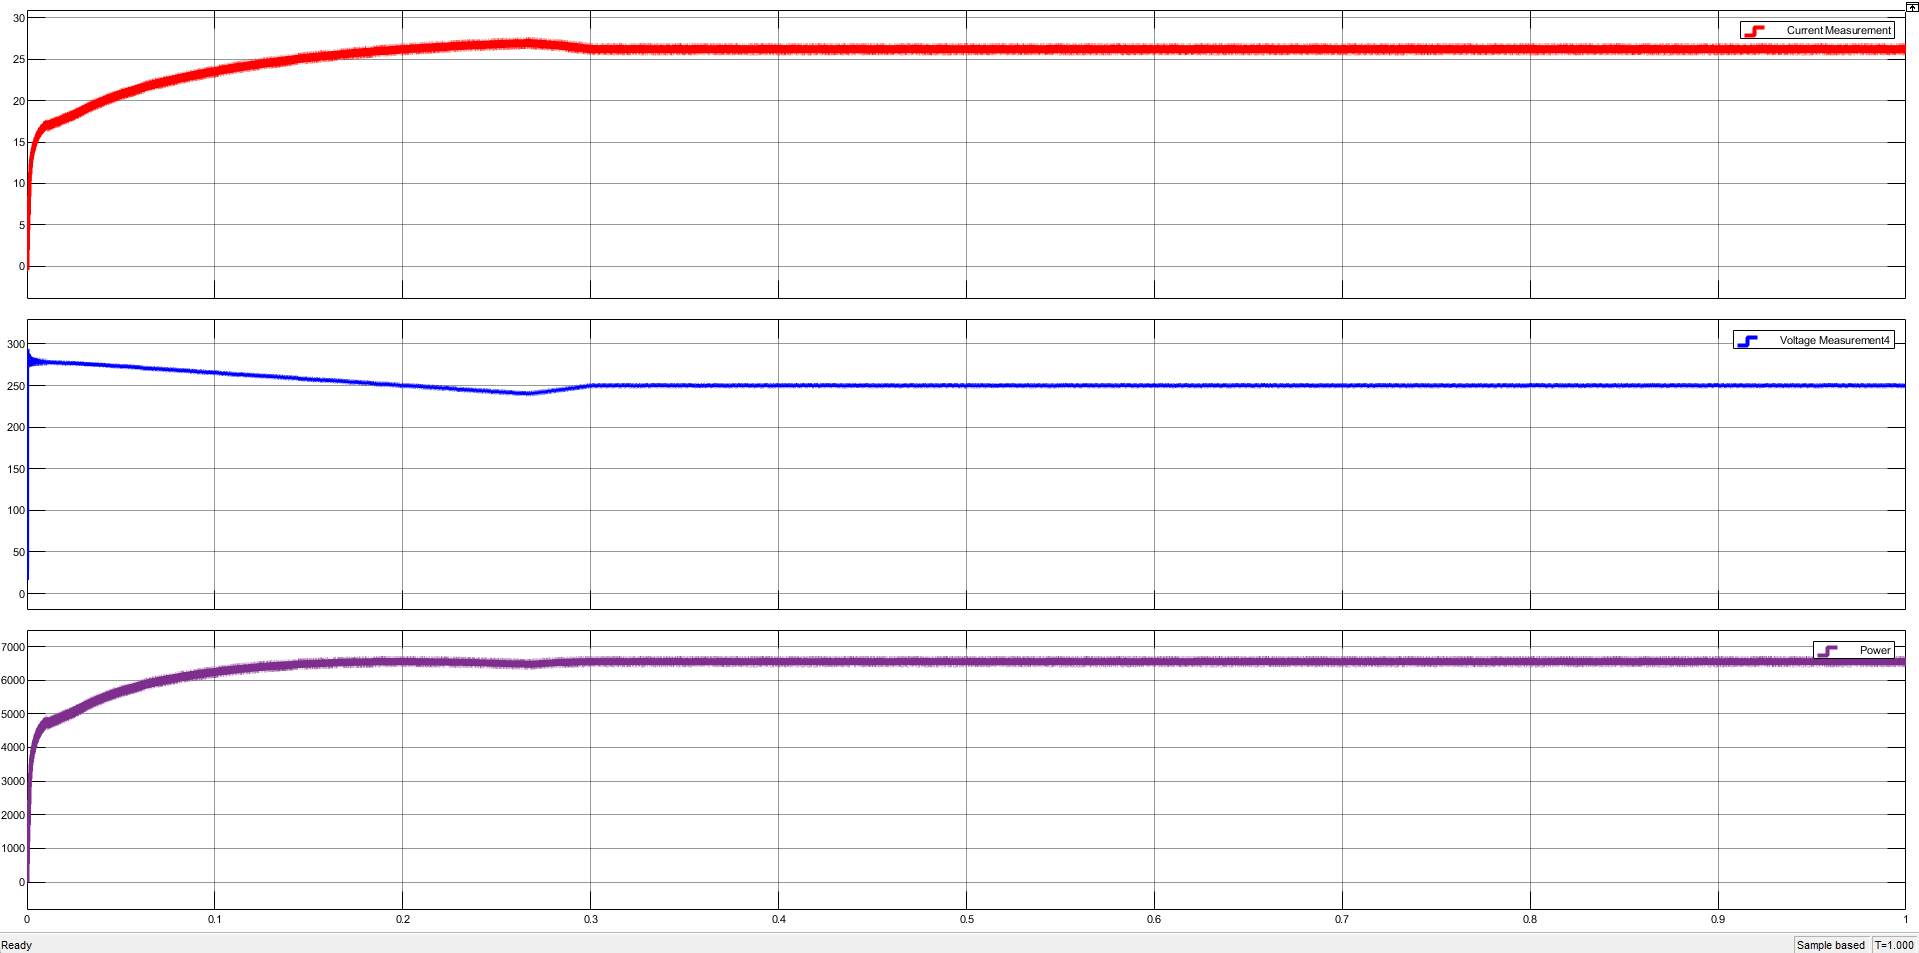
\includegraphics[width=1.1\textwidth]{Figures/5.1.15.png}
    \caption{Input current, voltage, power at 500 shading.}
    \label{fig:Input current, voltage, power at 500 shading}
\end{figure}
\begin{figure}[H]
    \centering
    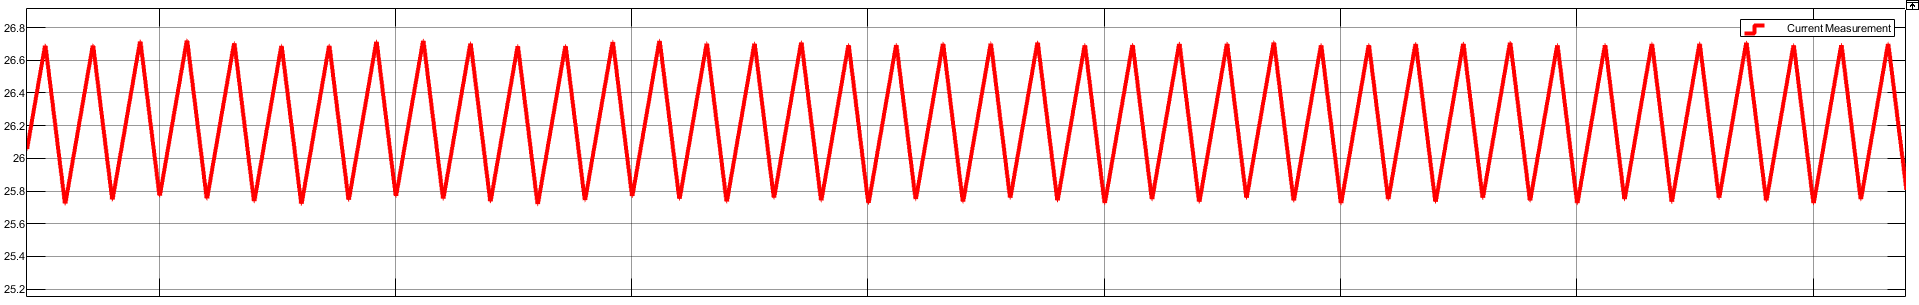
\includegraphics[width=1.1\textwidth]{Figures/5.1.16.png}
    \caption{Ripples of inductor current at 500 shading.}
    \label{fig:Ripples of inductor current at 500 shading}
\end{figure}
\begin{figure}[H]
    \centering
    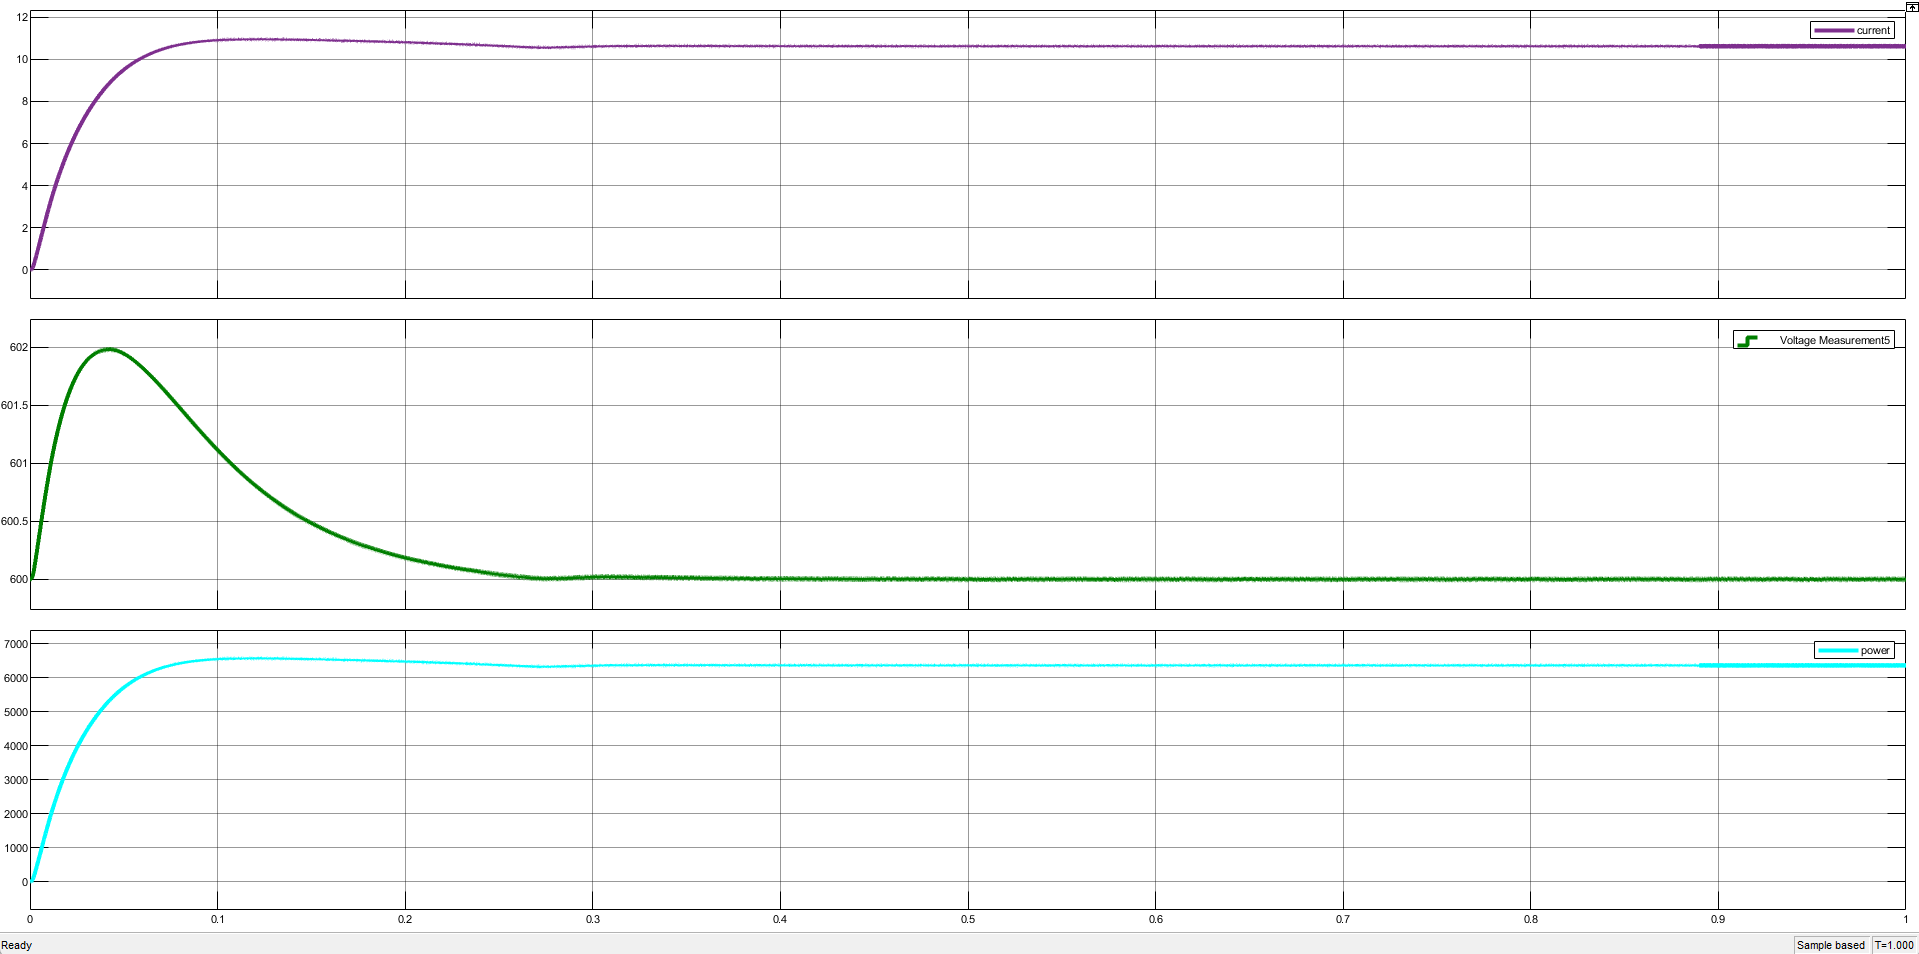
\includegraphics[width=1.1\textwidth]{Figures/5.1.17.png}
    \caption{Output current, voltage, power at 500 shading.}
    \label{fig:Output current, voltage, power at 500 shading}
\end{figure}
\subsubsection{Results of Simulation in Case of Shading (Ir = 250) at One Module}
\noindent
\begin{minipage}[t]{0.5\textwidth}
\vspace{0pt}
\begin{itemize}
  \item As shown, the output power decreases much more as the current decreases more than the current in the pervious case as Ir decreases, but the Vpv is almost constant.
  \item Dc link voltage still maintained at 600V due to closed loop with PI.
  \item Ripples of inductor current $= 22.2 - 21.4 = 0.8$\,A.
\end{itemize}
\end{minipage}
\hfill
\begin{minipage}[t]{0.4\textwidth}
\vspace{0pt}
  \centering
  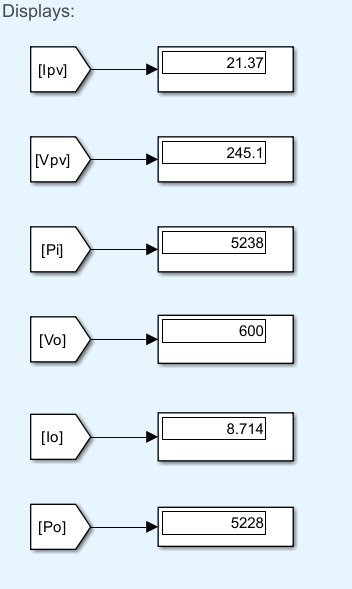
\includegraphics[width=\textwidth]{Figures/5.1.18.png}
  \captionof{figure}{Displays of central configuration at 250 shading.}
  \label{fig:Displays of central configuration at 250 shading}
\end{minipage}
\paragraph{Graphs}
\begin{figure}[H]
    \centering
    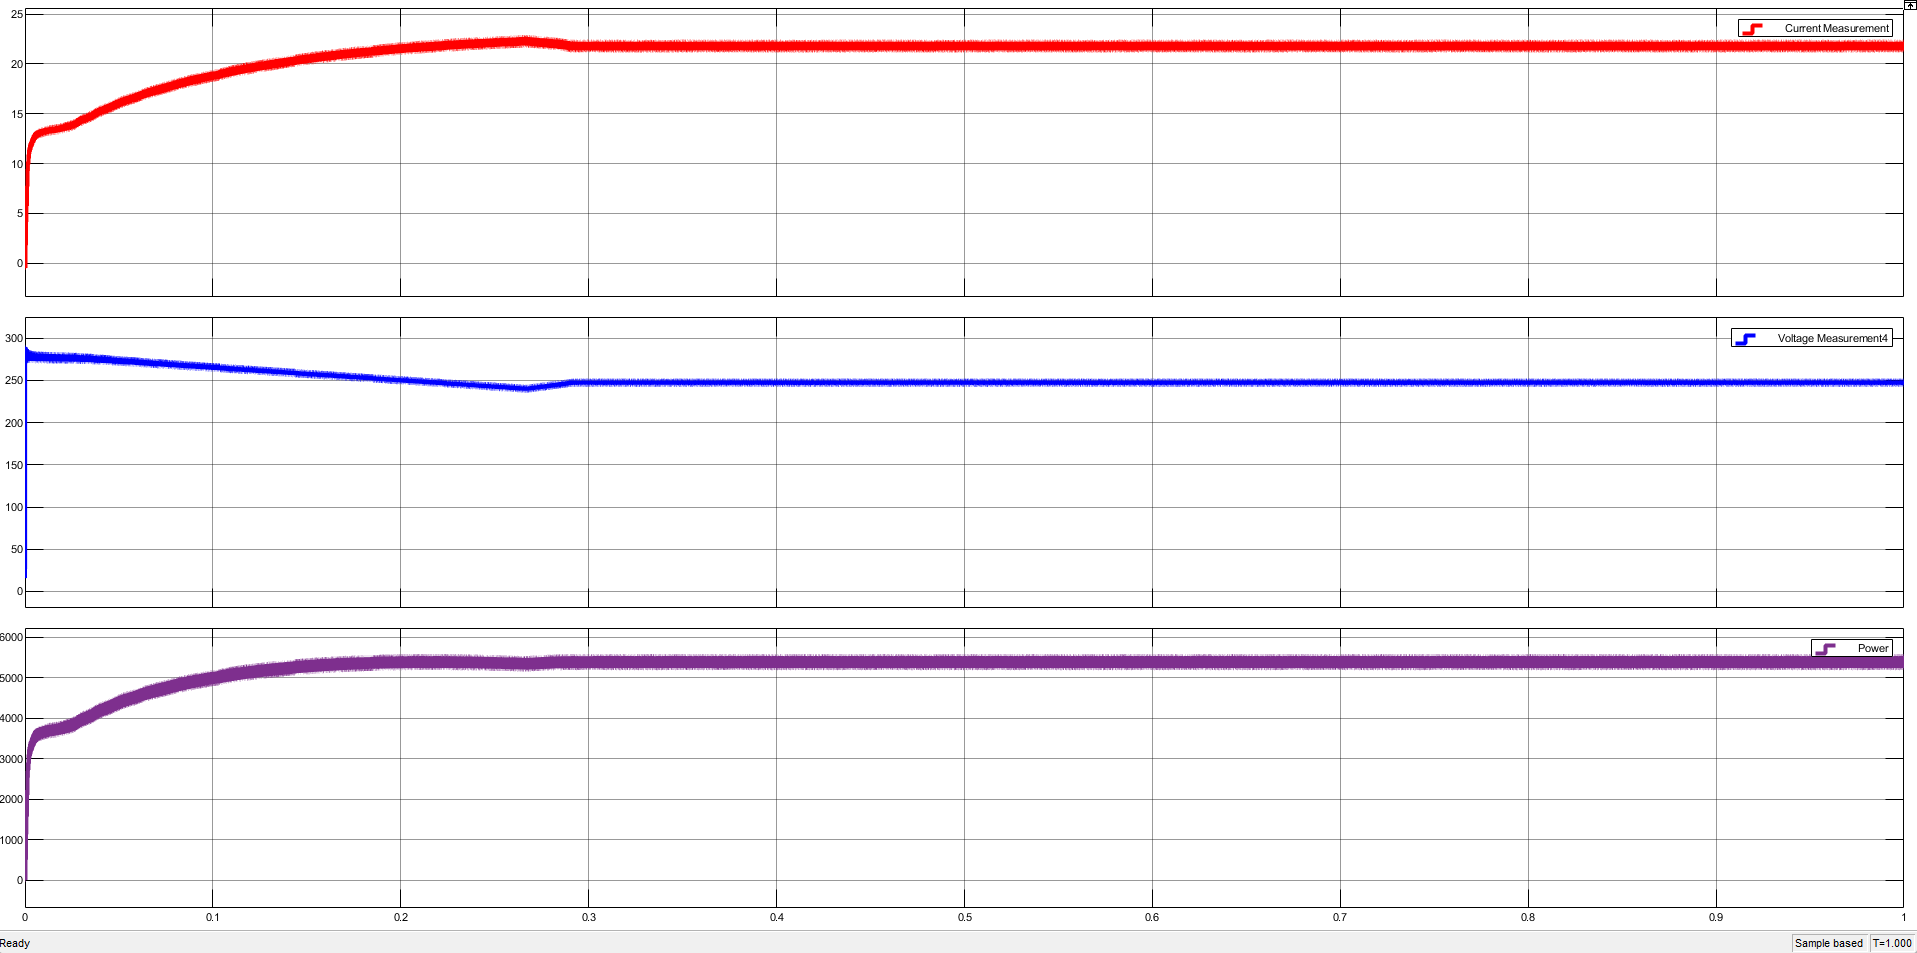
\includegraphics[width=1.1\textwidth]{Figures/5.1.19.png}
    \caption{Input current, voltage, power at 250 shading.}
    \label{fig:input current, voltage, power at 250 shading}
\end{figure}
\begin{figure}[H]
    \centering
    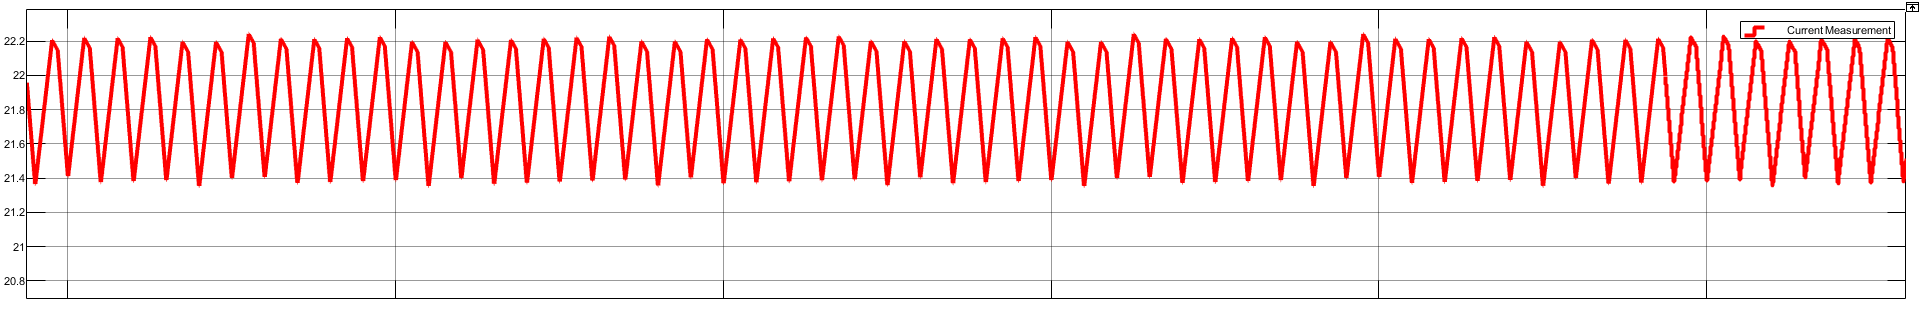
\includegraphics[width=1.1\textwidth]{Figures/5.1.20.png}
    \caption{Ripples of inductor current at 250 shading.}
    \label{fig:ripples of inductor current at 250 shading}
\end{figure}
\begin{figure}[H]
    \centering
    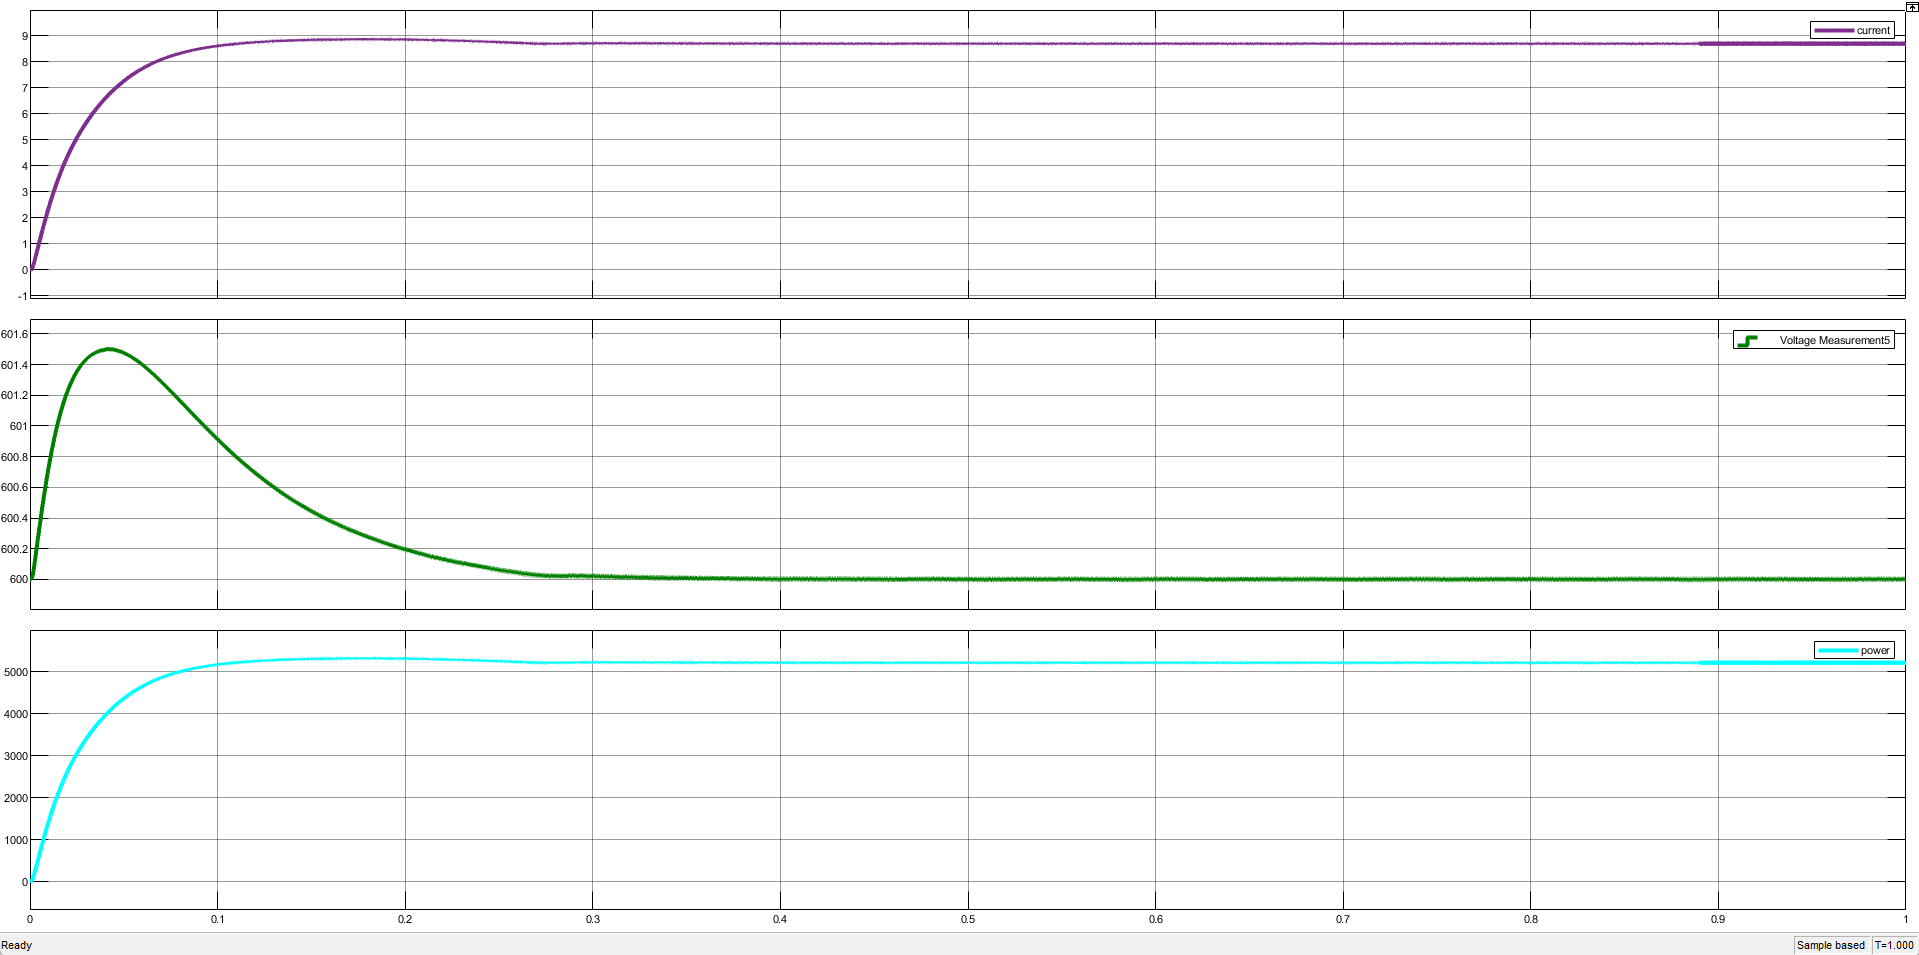
\includegraphics[width=1.1\textwidth]{Figures/5.1.21.png}
    \caption{Output current, voltage, power at 250 shading.}
    \label{fig:Output current, voltage, power at 250 shading}
\end{figure}


\subsection{String Configuration with Load}
String Array configuration is the same idea but with boost converter with each leg, all connected to the same DC link.
\begin{figure}[H]
    \centering
    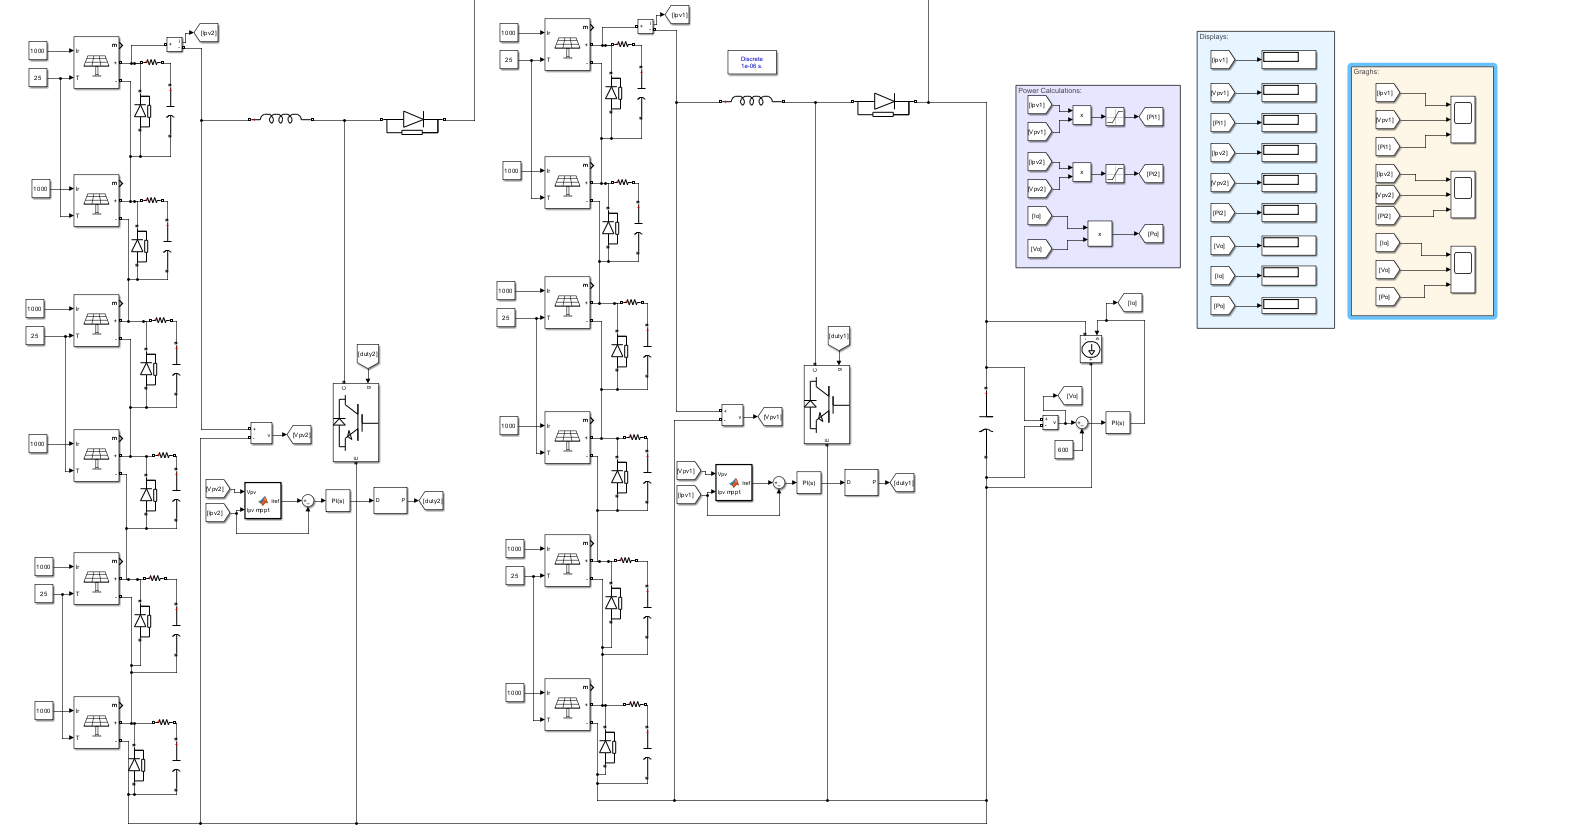
\includegraphics[width=1\textwidth]{Figures/5.1.22.png}
    \caption{String array configuration.}
    \label{fig:String array configuration}
\end{figure}
\subsubsection{Results of Simulation in Case of No Shading}
\noindent
\begin{minipage}[t]{0.5\textwidth}
\vspace{0pt}
\begin{itemize}
  \item The power is slightly less than in case of central at maximum power, the cause of this might be the more switching devices used as there are two converters instead of one.

  \item Dc link voltage still maintained at 600\,V due to closed loop with PI  
        ($K_p = 5$, $K_i = 90$). 

  \item Ripples of inductor current of string 1 $= 17.8 - 16.9 = 0.9$\,A.\
  \item Ripples of inductor current of string 2 $= 17.8 - 16.9 = 0.9$\,A.\
\end{itemize}
\end{minipage}
\hfill
\begin{minipage}[t]{0.3\textwidth}
\vspace{0pt}
  \centering
  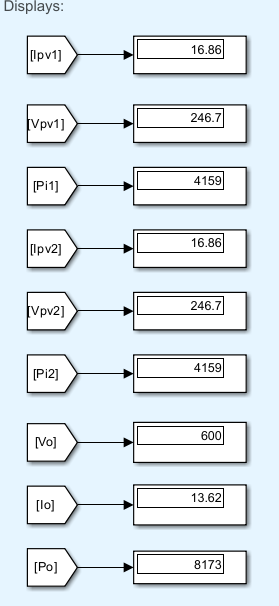
\includegraphics[width=\textwidth]{Figures/5.1.23.png}
  \captionof{figure}{Displays of string configuration at no shading.}
  \label{fig:Displays of string configuration at no shading}
\end{minipage}
\paragraph{Graphs}
\begin{figure}[H]
    \centering
    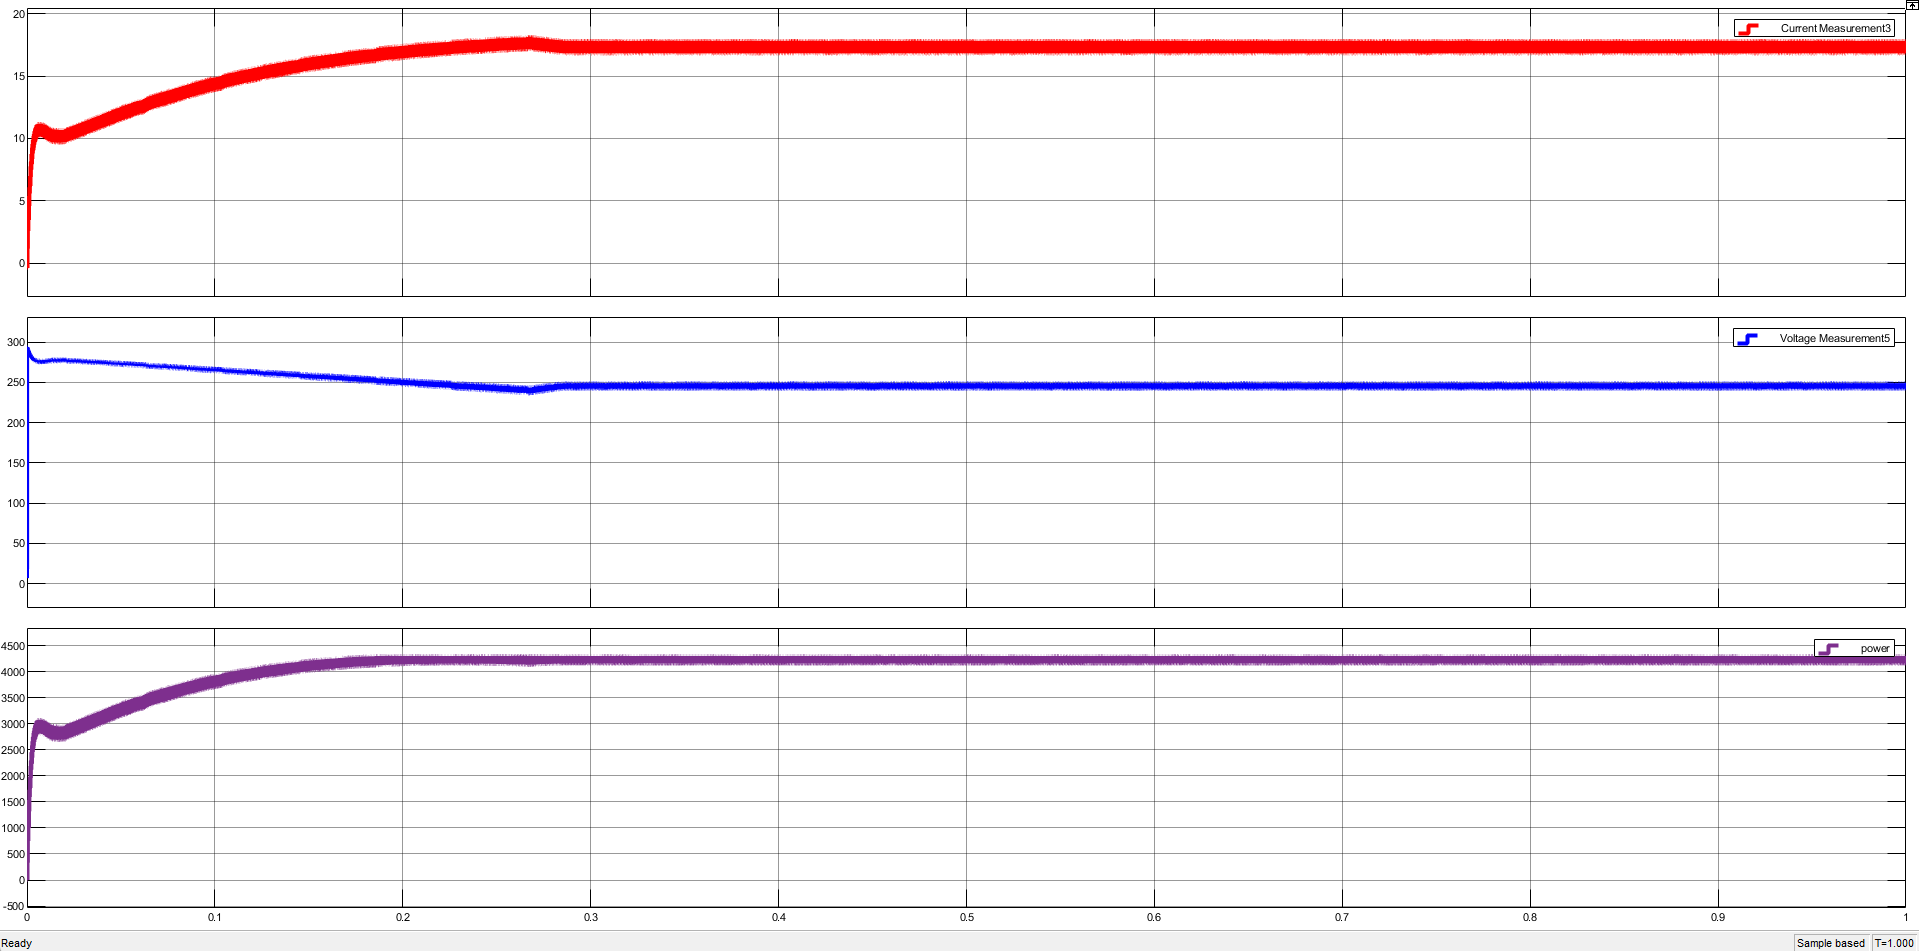
\includegraphics[width=1\textwidth]{Figures/5.1.24.png}
    \caption{Input current, voltage, power at string 1 at no shading.}
    \label{fig:input current, voltage, power at string 1 at no shading}
\end{figure}
\begin{figure}[H]
    \centering
    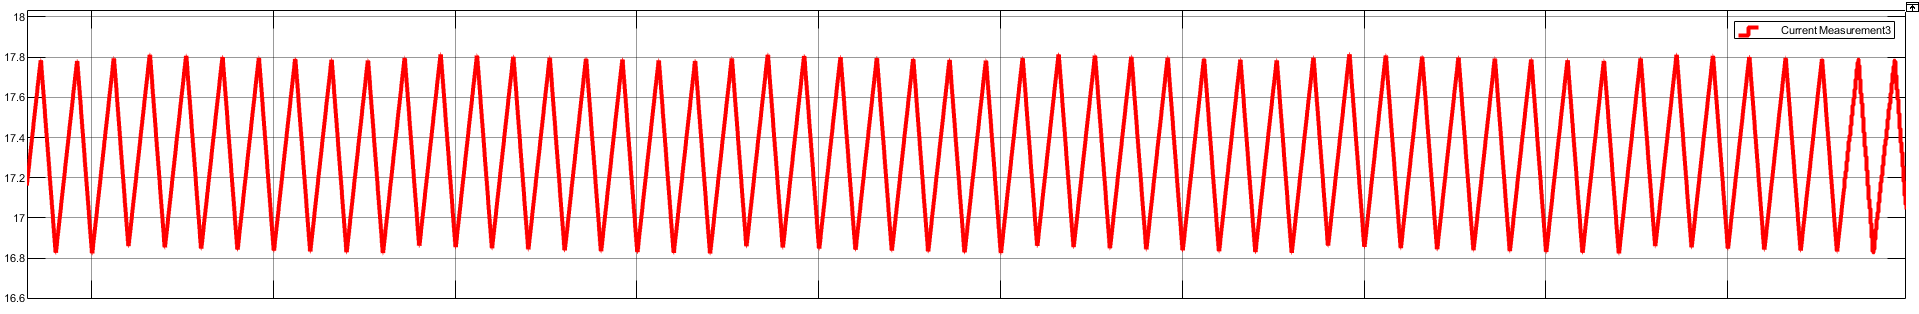
\includegraphics[width=1\textwidth]{Figures/5.1.25.png}
    \caption{Ripples of inductor current of string 1 at no shading.}
    \label{fig:Ripples of inductor current of string 1 at no shading}
\end{figure}
\begin{figure}[H]
    \centering
    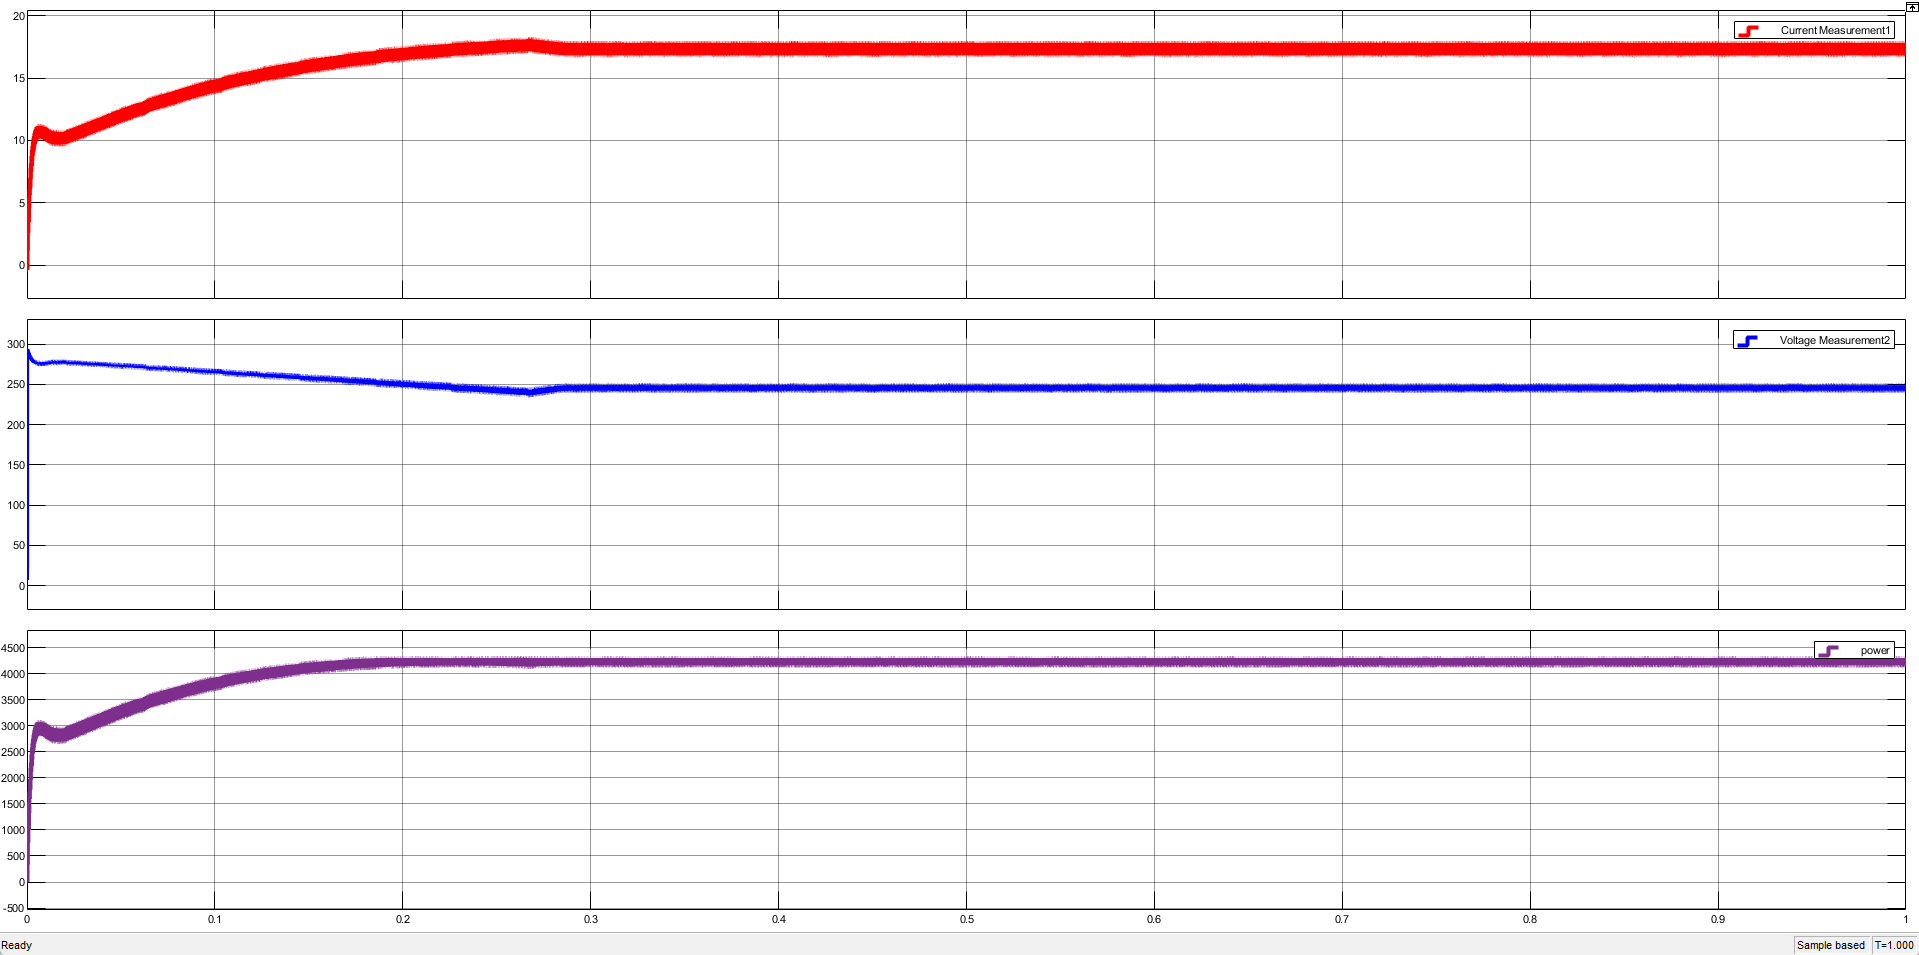
\includegraphics[width=1\textwidth]{Figures/5.1.26.png}
    \caption{Input current, voltage, power at string 2 at no shading.}
    \label{fig:input current, voltage, power at string 2 at no shading}
\end{figure}
\begin{figure}[H]
    \centering
    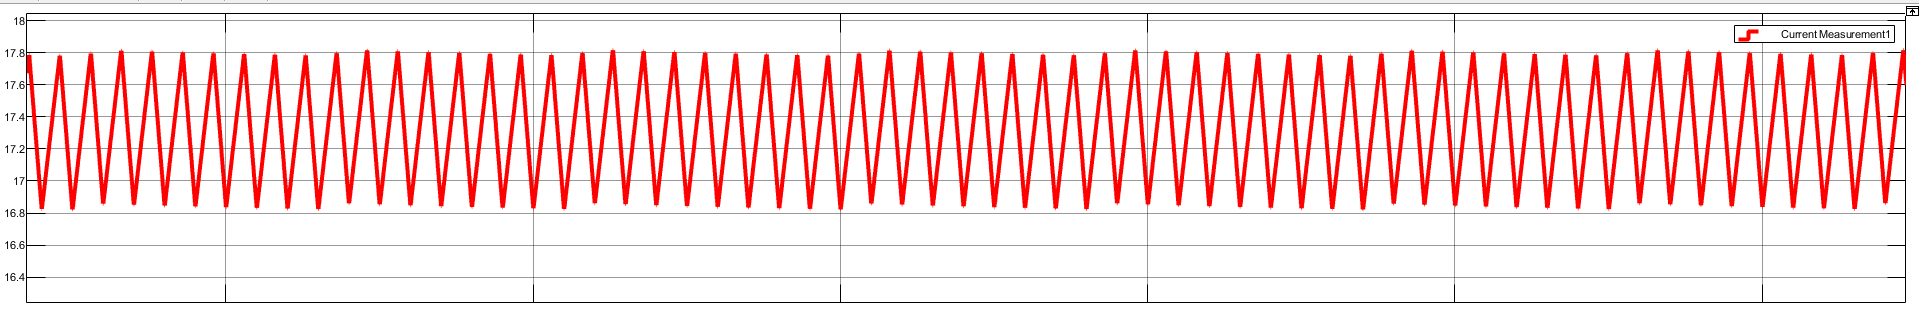
\includegraphics[width=1\textwidth]{Figures/5.1.27.png}
    \caption{Ripples of inductor current of string 2 at no shading.}
    \label{fig:ripples of inductor current of string 2 at no shading}
\end{figure}
\begin{figure}[H]
    \centering
    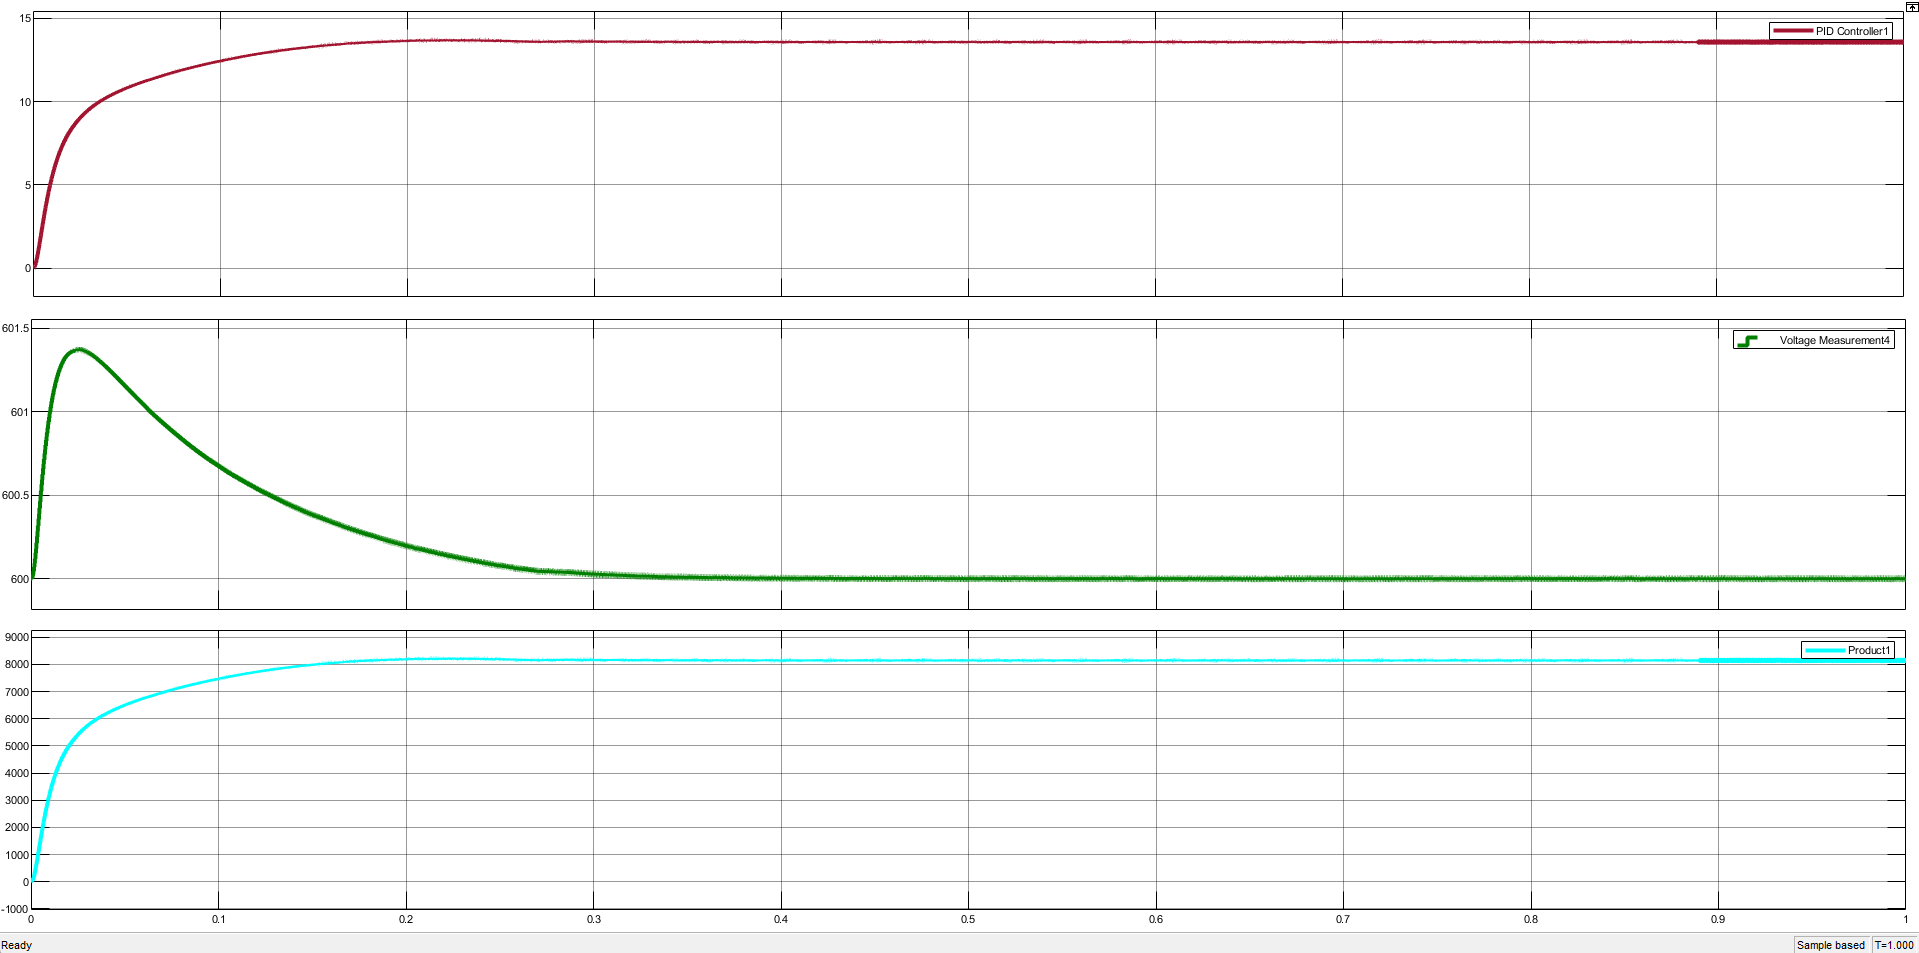
\includegraphics[width=1\textwidth]{Figures/5.1.28.png}
    \caption{Output current, voltage, power at no shading.}
    \label{fig:Output current, voltage, power at no shading}
\end{figure}

\subsubsection{Results of Simulation in Case of Shading (Ir = 800) at One Module at One String}
\noindent
\begin{minipage}[t]{0.5\textwidth}
\vspace{0pt}
\begin{itemize}
  \item As shown, the output power decreases as the current decreases only in the string that has shaded module, but the other string is unshaded, so it outputs the max power.
\item As shown, the output power in string configuration is more than the output power in central configuration and this is the key difference between them and why is string is better in shading.
  \item Dc link voltage still maintained at 600\,V due to closed loop with PI.  

  \item Ripples of inductor current of string 1 $= 17.8 - 16.9 = 0.9$\,A.\
  \item Ripples of inductor current of string 2 $= 15 - 14 = 1$\,A.\
\end{itemize}
\end{minipage}
\hfill
\begin{minipage}[t]{0.3\textwidth}
\vspace{0pt}
  \centering
  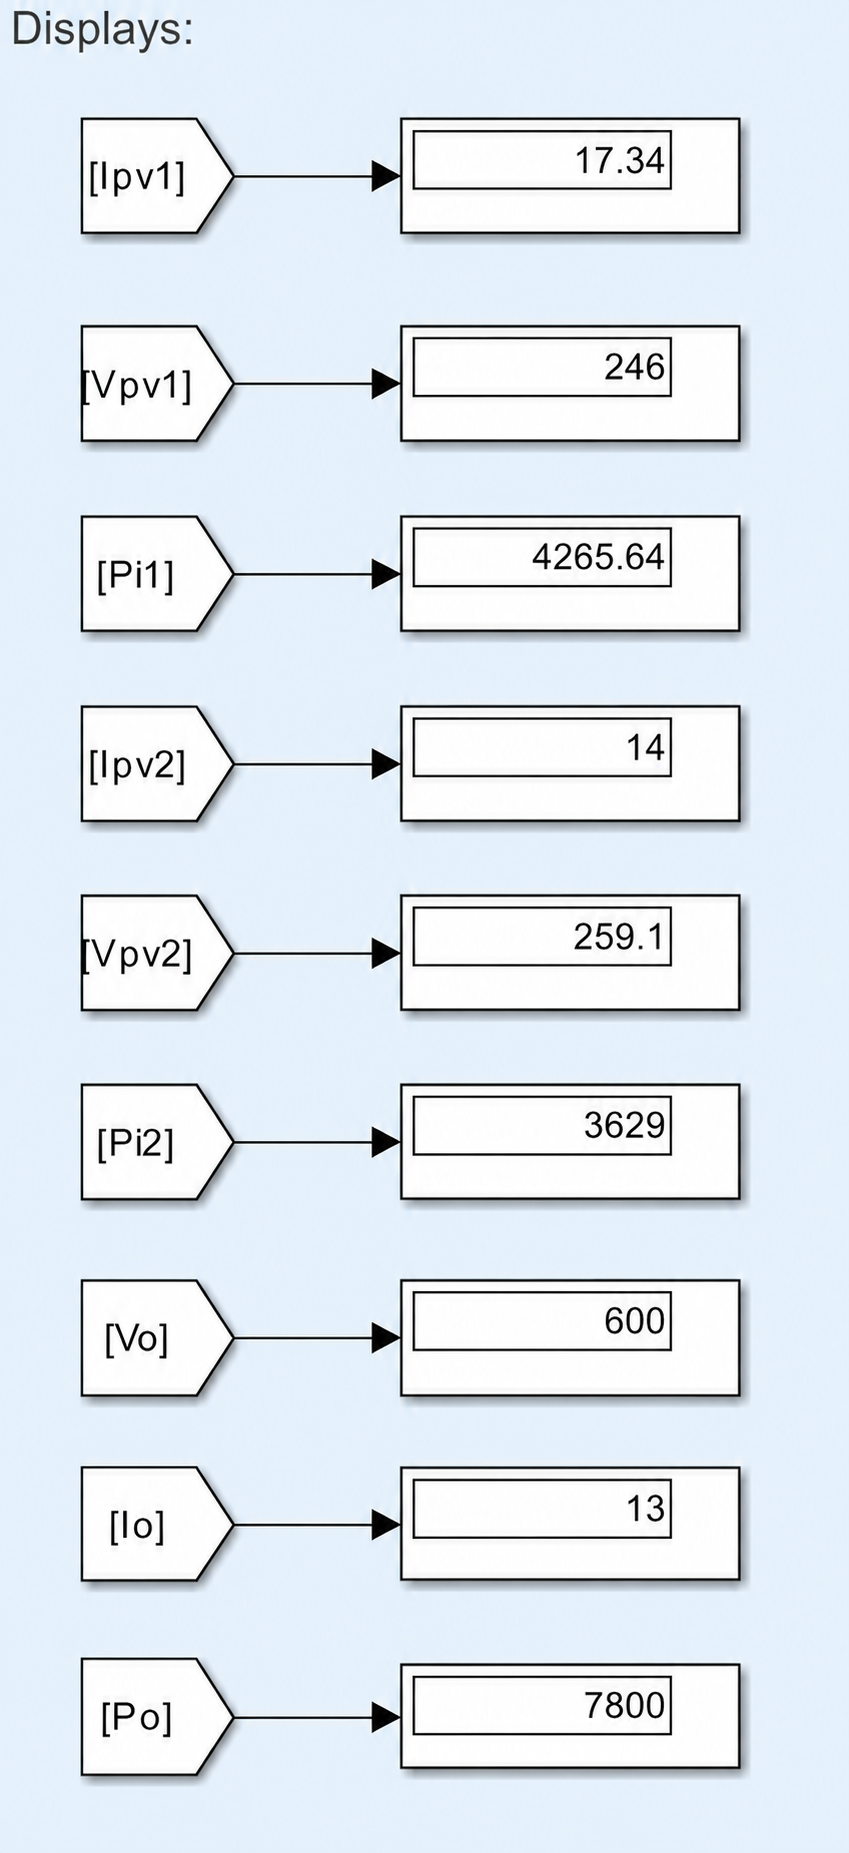
\includegraphics[width=\textwidth]{Figures/5.1.70.png}
  \captionof{figure}{Displays of string configuration at 800 shading.}
  \label{fig:Displays of string configuration at 800 shading}
\end{minipage}
\paragraph{Graphs}
\begin{figure}[H]
    \centering
    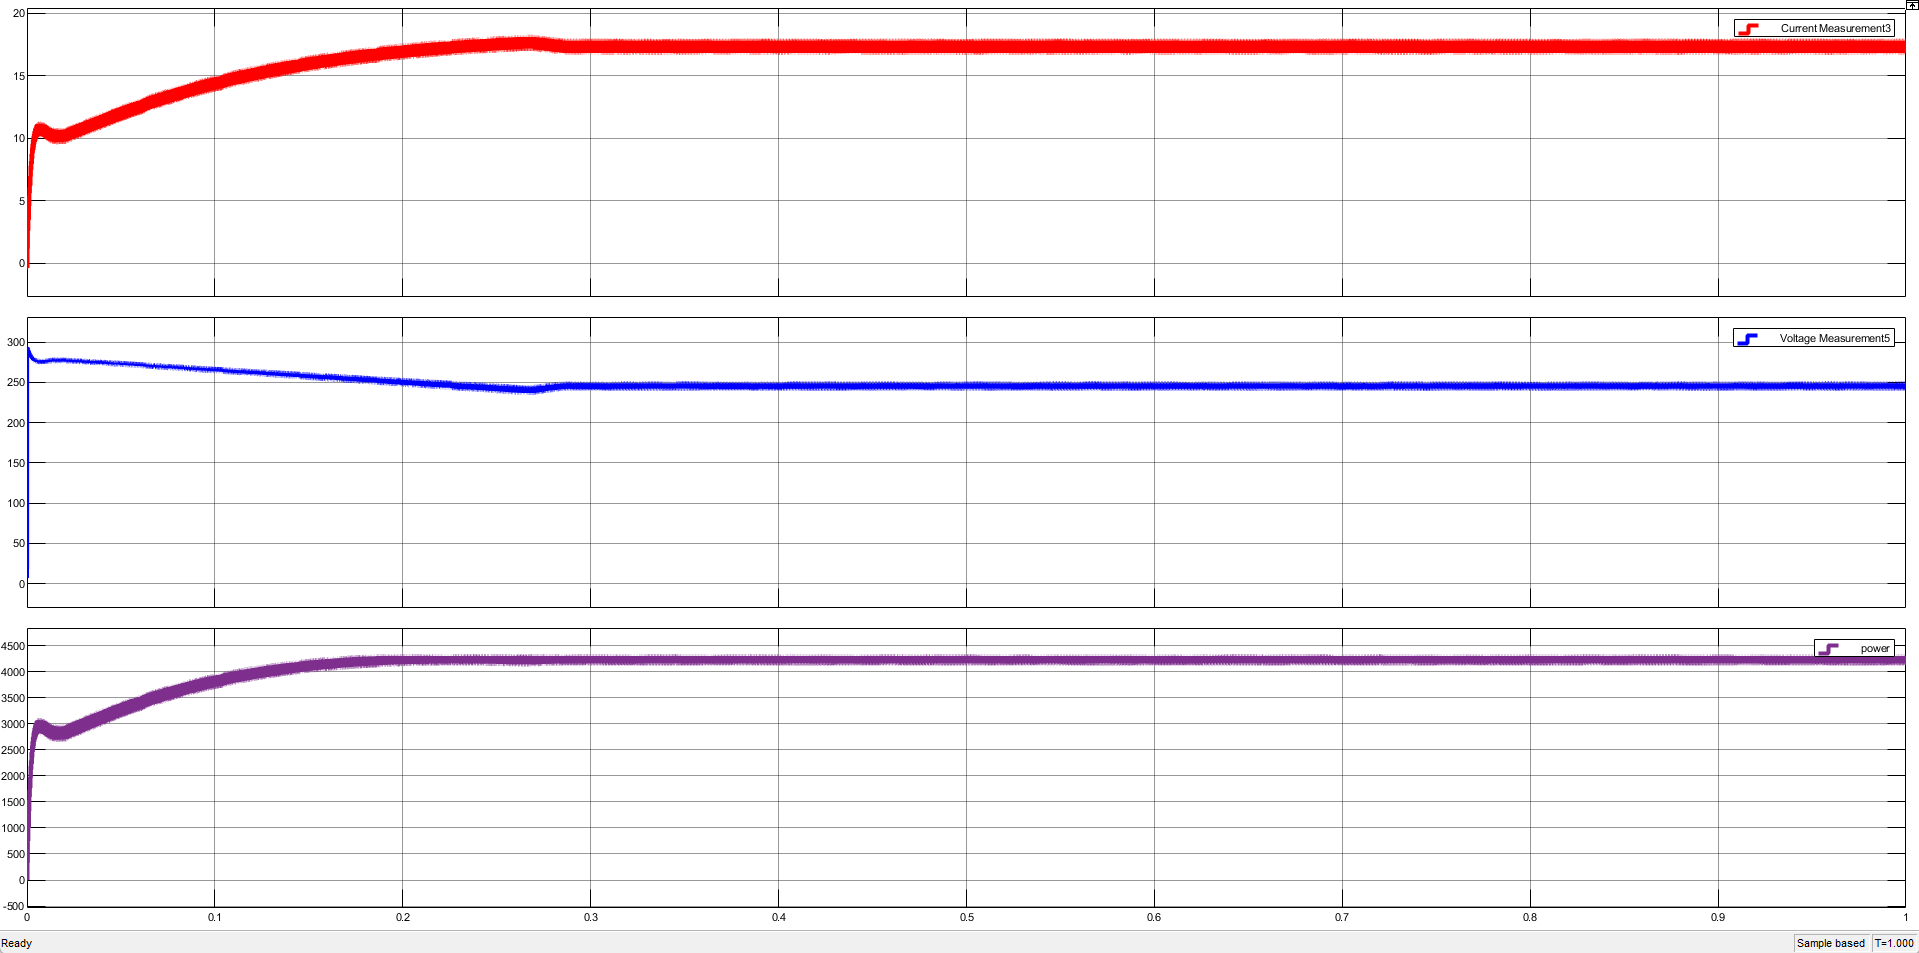
\includegraphics[width=1\textwidth]{Figures/5.1.30.png}
    \caption{Input current, voltage, power at string 1 at 800 shading.}
    \label{fig:input current, voltage, power at string 1 at 800 shading}
\end{figure}
\begin{figure}[H]
    \centering
    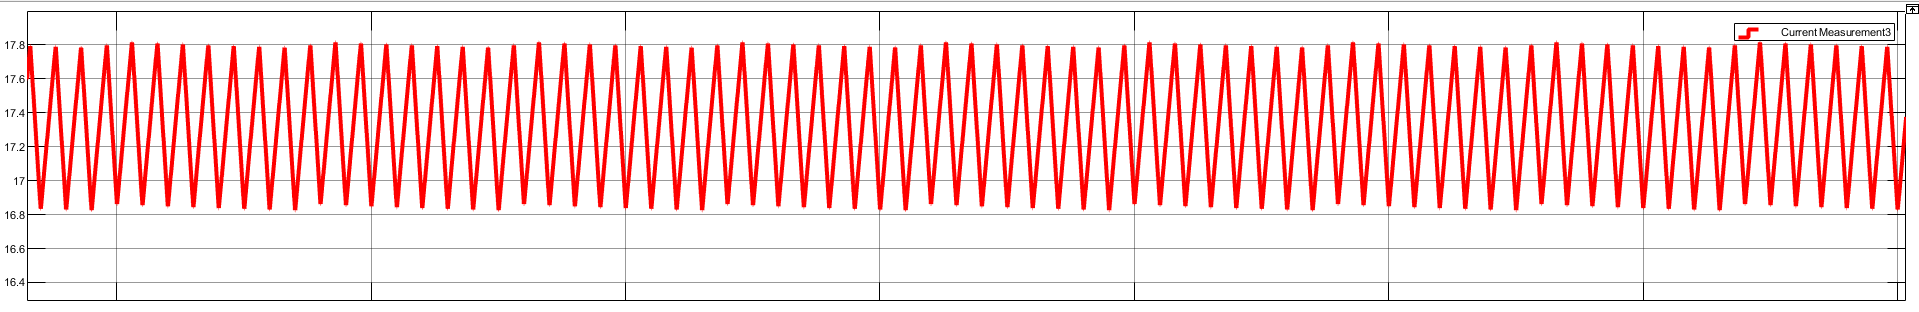
\includegraphics[width=1\textwidth]{Figures/5.1.31.png}
    \caption{Ripples of inductor current of string 1 at 800 shading.}
    \label{fig:ripples of inductor current of string 1 at 800 shading}
\end{figure}
\begin{figure}[H]
    \centering
    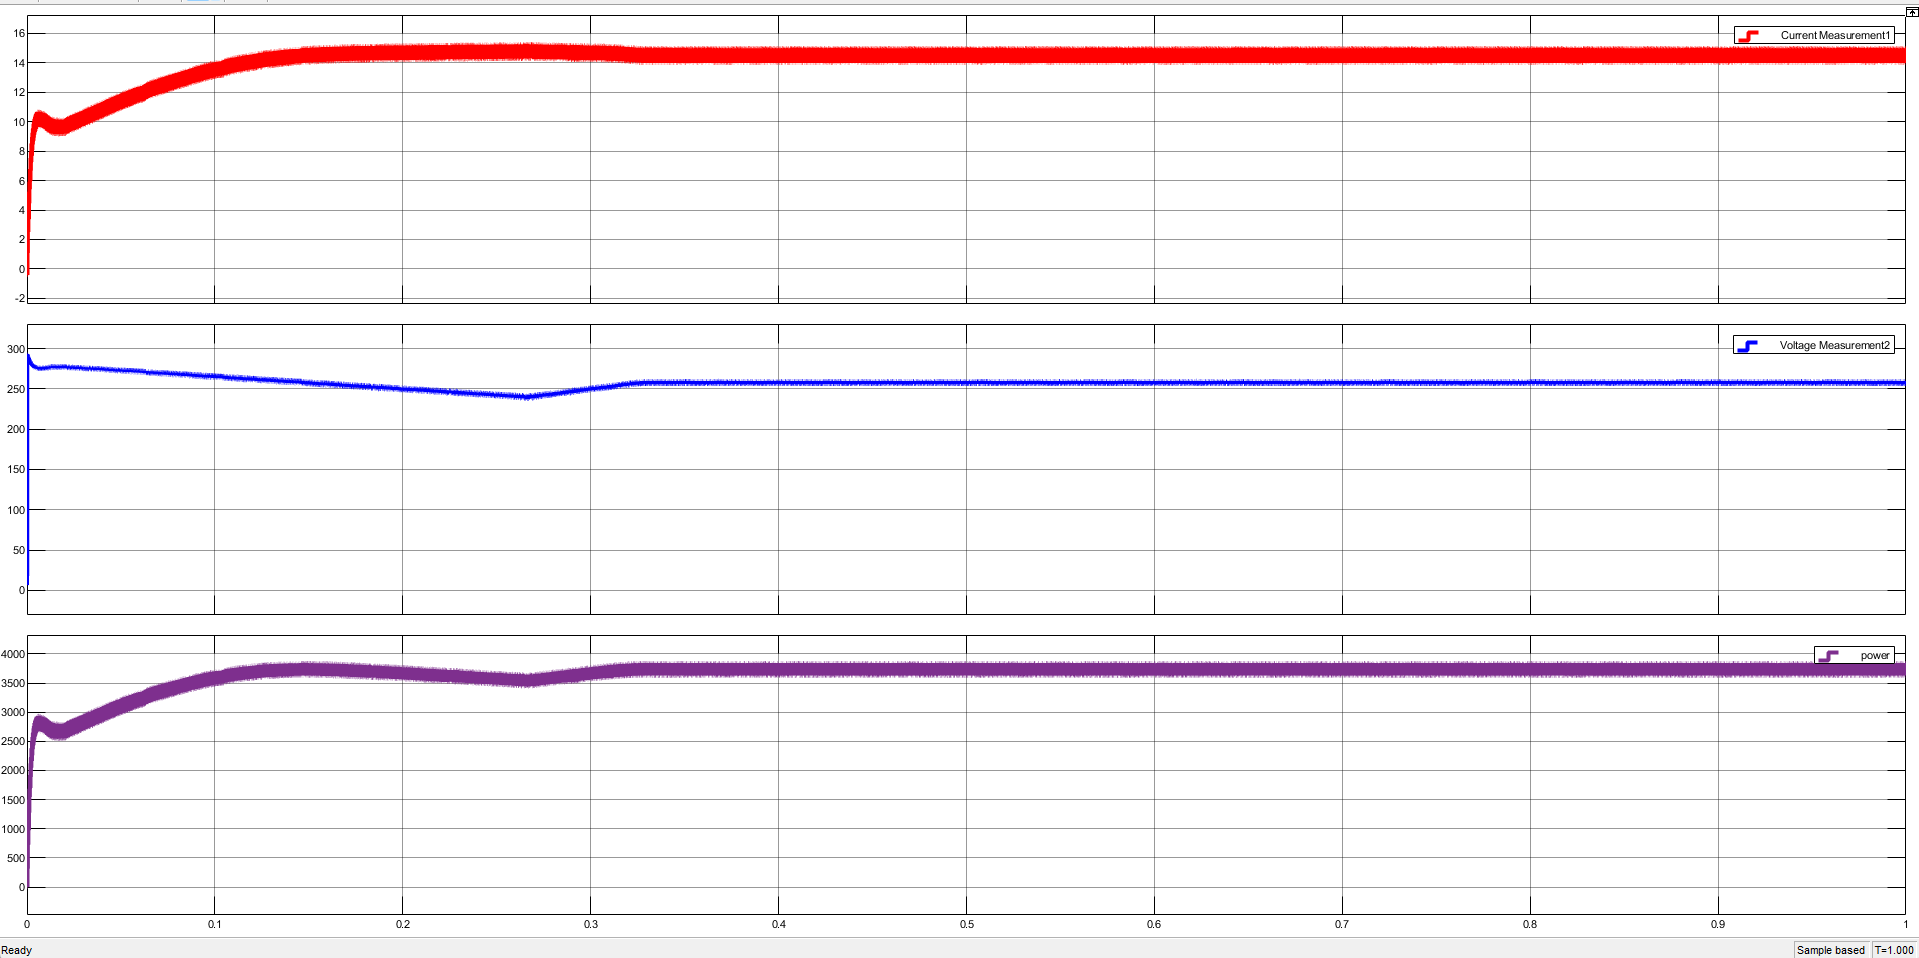
\includegraphics[width=1\textwidth]{Figures/5.1.32.png}
    \caption{Input current, voltage, power at string 2 at 800 shading.}
    \label{fig:input current, voltage, power at string 2 at 800 shading}
\end{figure}
\begin{figure}[H]
    \centering
    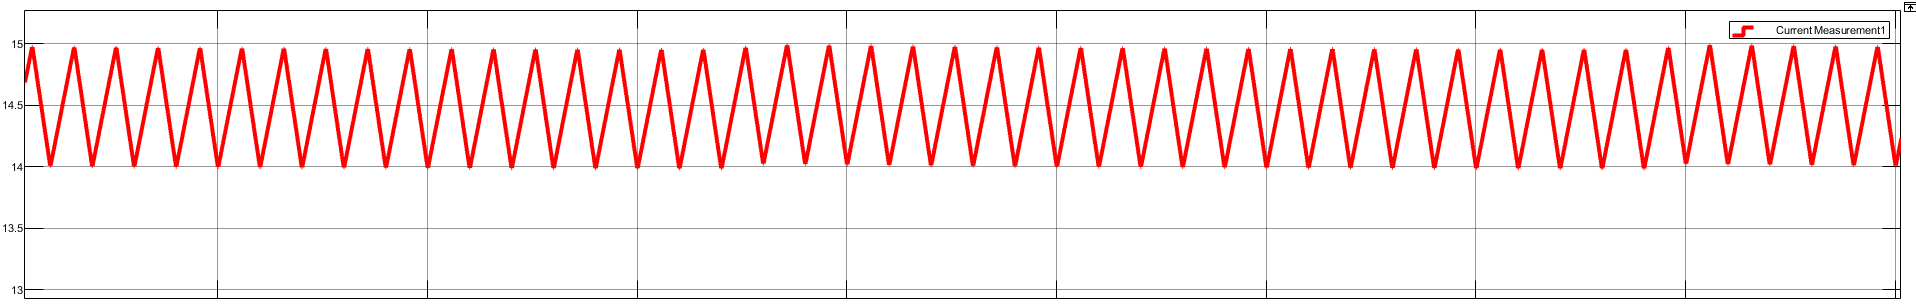
\includegraphics[width=1\textwidth]{Figures/5.1.33.png}
    \caption{Ripples of inductor current of string 2 at 800 shading.}
    \label{fig:ripples of inductor current of string 2 at 800 shading}
\end{figure}
\begin{figure}[H]
    \centering
    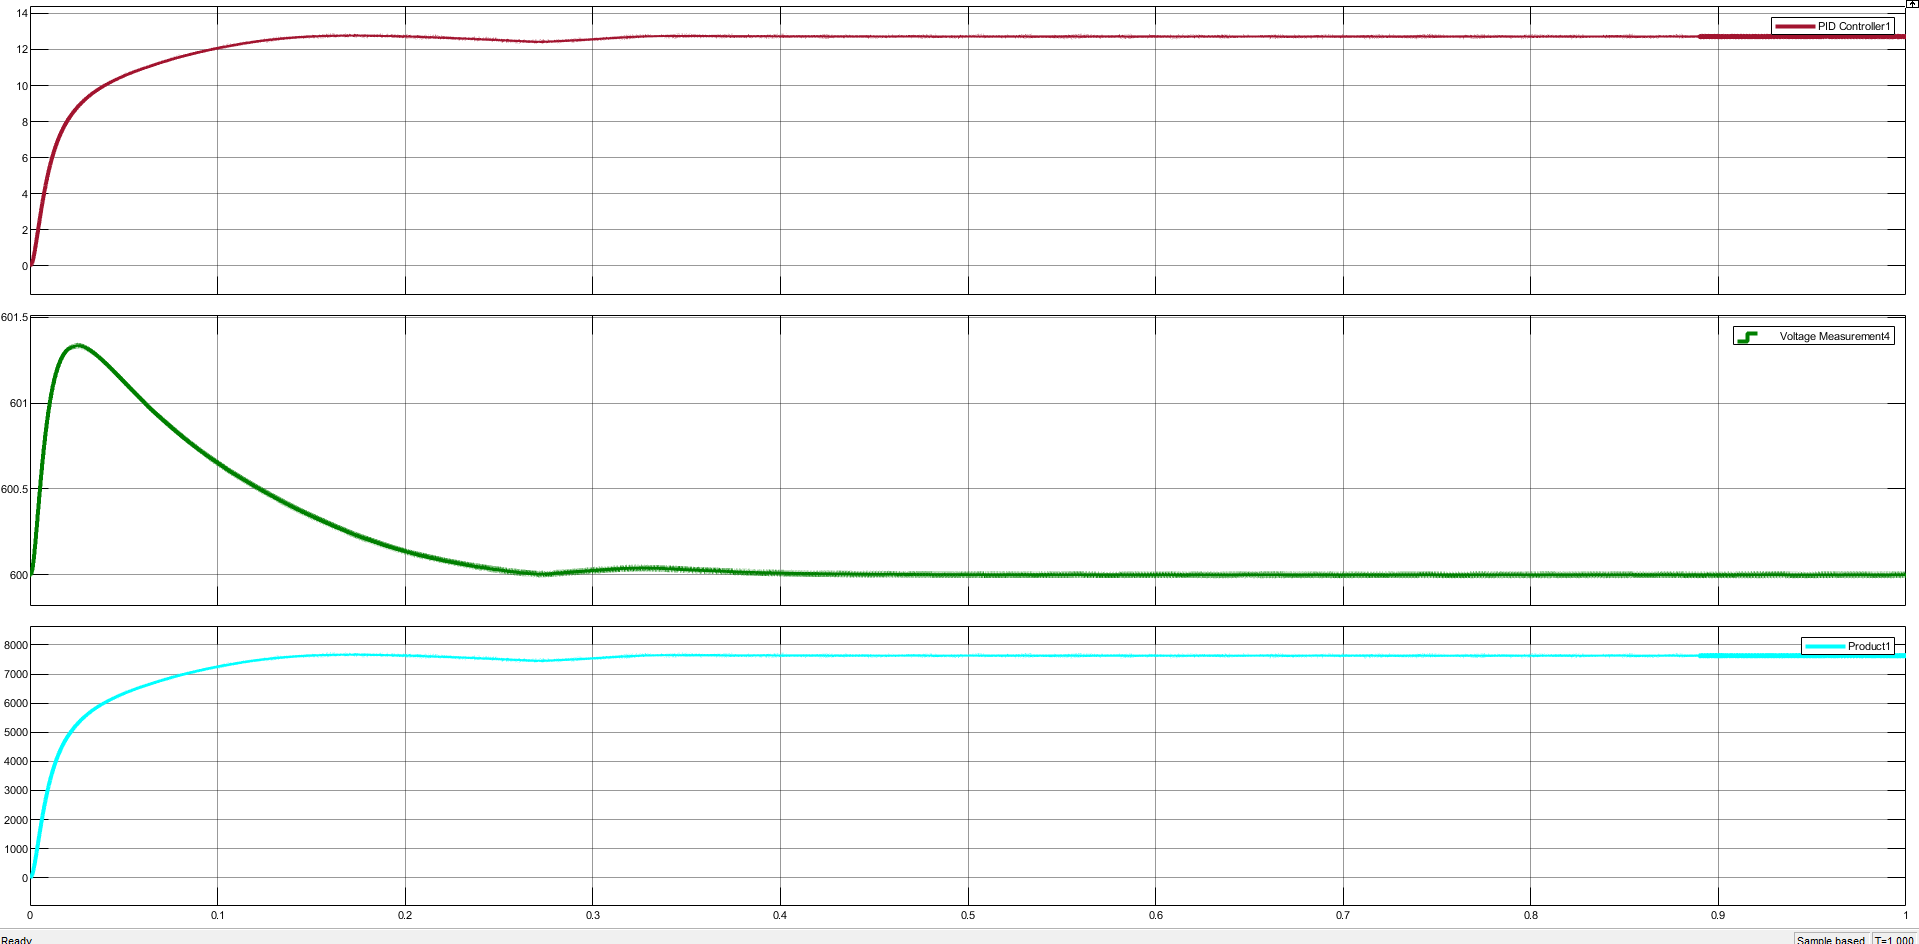
\includegraphics[width=1\textwidth]{Figures/5.1.34.png}
    \caption{Output current, voltage, power at 800 shading.}
    \label{fig:Output current, voltage, power at 800 shading}
\end{figure}

\subsubsection{Results of Simulation in Case of Shading (Ir = 500) at One Module at One String}
\noindent
\begin{minipage}[t]{0.5\textwidth}
\vspace{0pt}
\begin{itemize}
  \item As shown, the output power decreases as the current decreases only in the string that has shaded module, but the other string is unshaded, so it outputs the max power.
  \item As shown, the output power in string configuration is more than the output power in central configuration and this is the key difference between them and why is string is better in shading.
  \item Dc link voltage still maintained at 600\,V due to closed loop with PI.  

  \item Ripples of inductor current of string 1 $= 17.5 - 16.6 = 0.9$\,A.\
  \item Ripples of inductor current of string 2 $= 9.7 - 8.8 = 0.9$\,A.\
\end{itemize}
\end{minipage}
\hfill
\begin{minipage}[t]{0.3\textwidth}
\vspace{0pt}
  \centering
  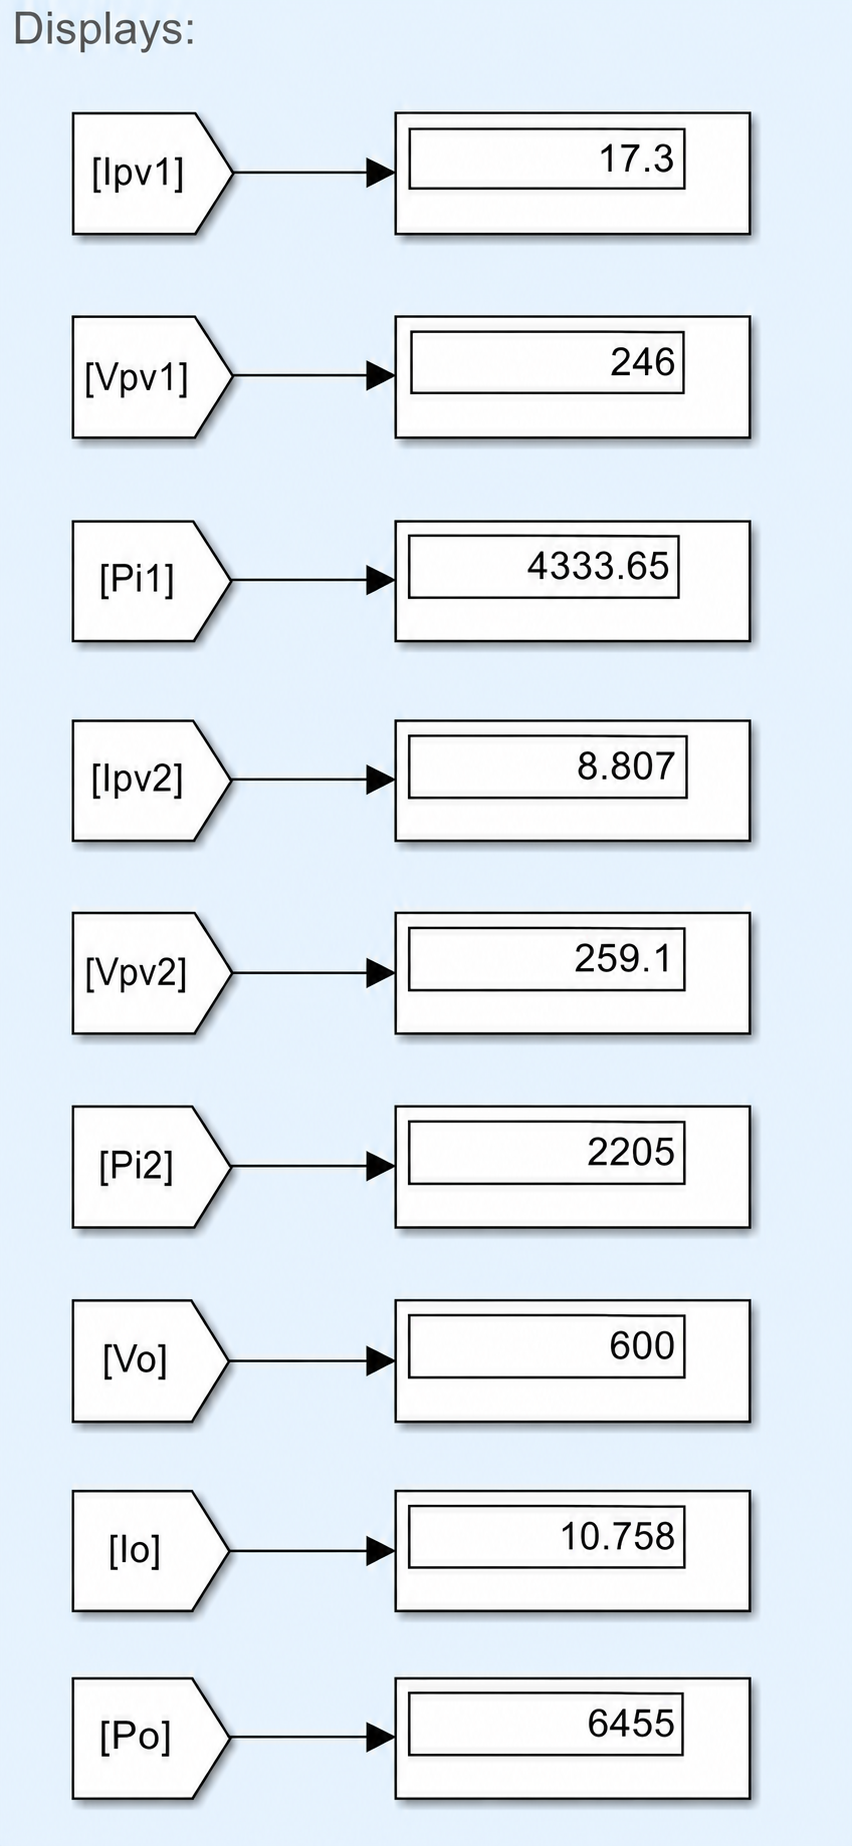
\includegraphics[width=\textwidth]{Figures/5.1.71.png}
  \captionof{figure}{Displays of string configuration at 500 shading.}
  \label{fig:Displays of string configuration at 500 shading}
\end{minipage}
\paragraph{Graphs}
\begin{figure}[H]
    \centering
    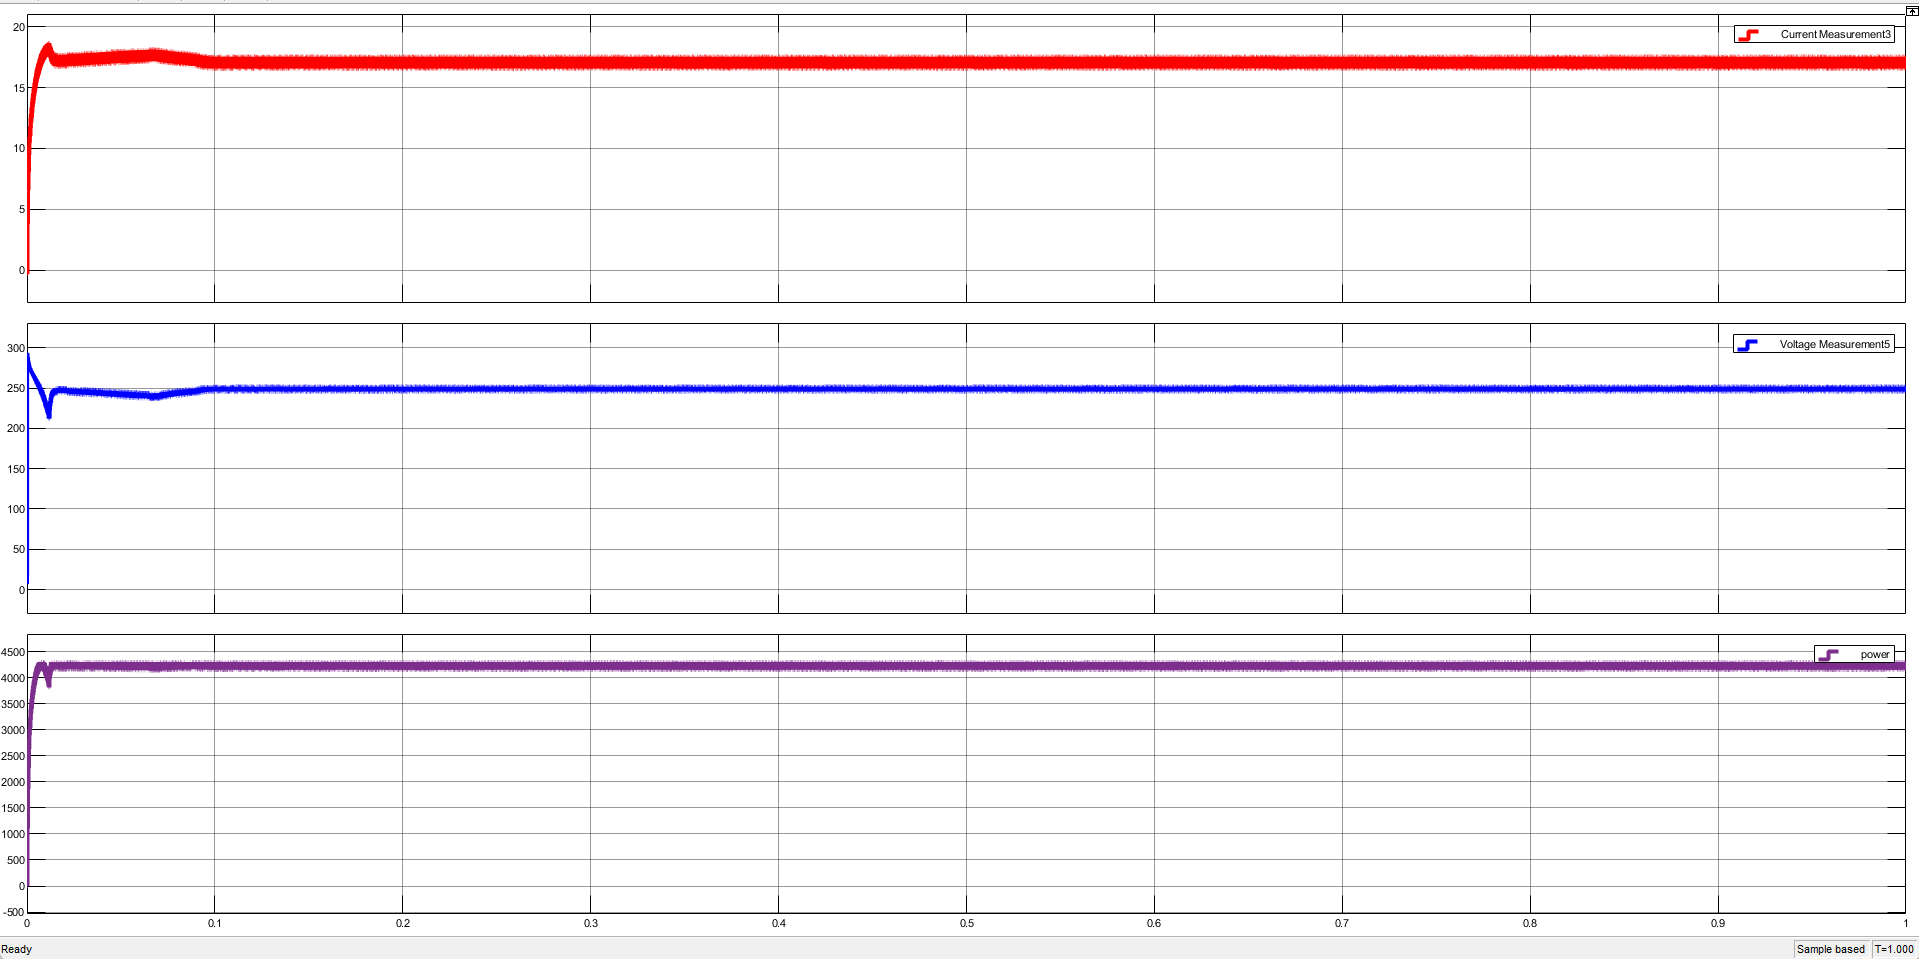
\includegraphics[width=1\textwidth]{Figures/5.1.36.png}
    \caption{Input current, voltage, power at string 1 at 500 shading.}
    \label{fig:input current, voltage, power at string 1 at 500 shading}
\end{figure}
\begin{figure}[H]
    \centering
    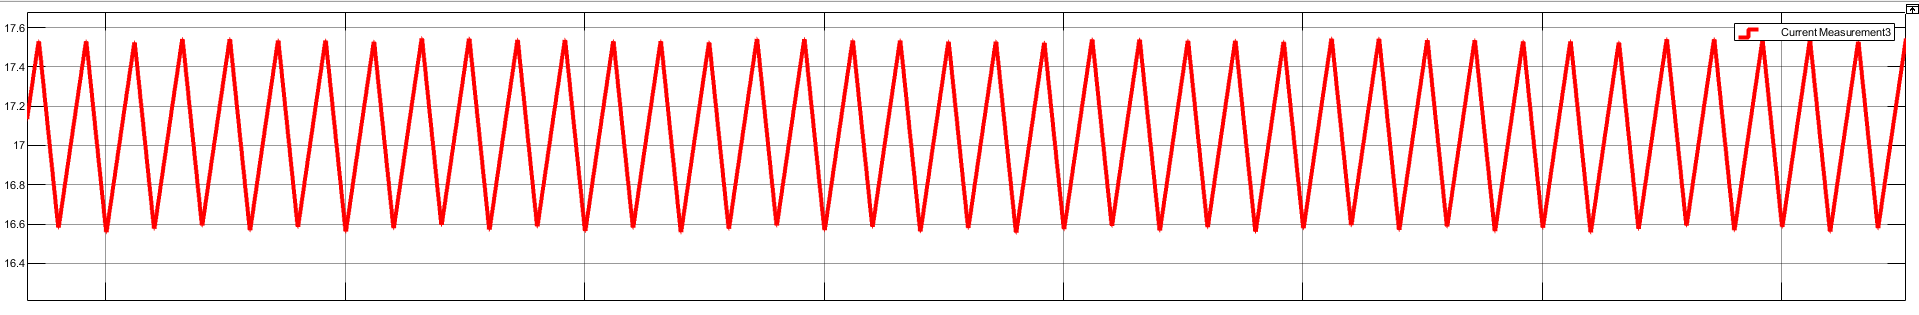
\includegraphics[width=1\textwidth]{Figures/5.1.37.png}
    \caption{Ripples of inductor current of string 1 at 500 shading.}
    \label{fig:ripples of inductor current of string 1 at 500 shading}
\end{figure}
\begin{figure}[H]
    \centering
    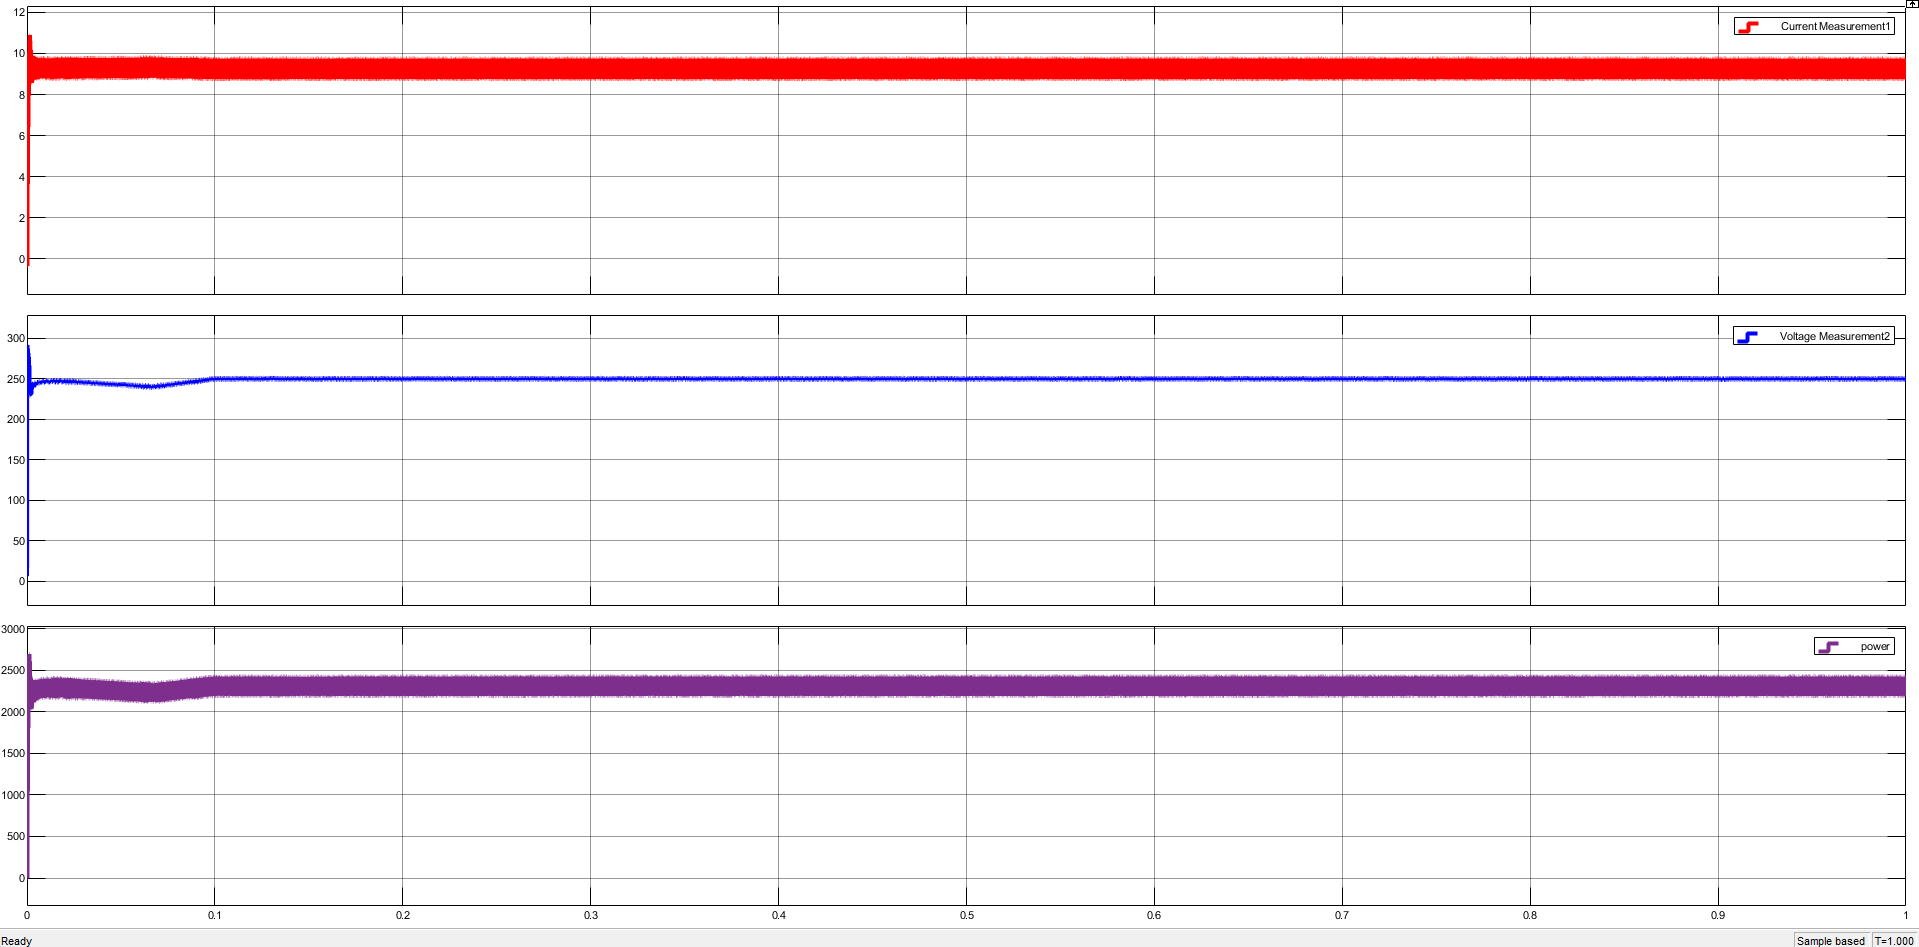
\includegraphics[width=1\textwidth]{Figures/5.1.38.png}
    \caption{Input current, voltage, power at string 2 at 500 shading.}
    \label{fig:input current, voltage, power at string 2 at 500 shading}
\end{figure}
\begin{figure}[H]
    \centering
    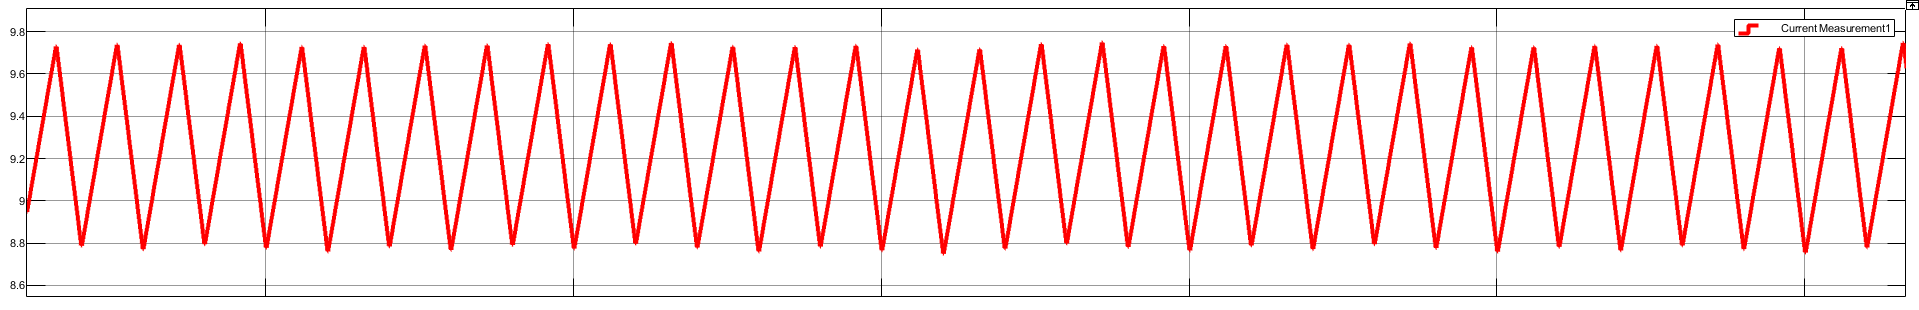
\includegraphics[width=1\textwidth]{Figures/5.1.39.png}
    \caption{Ripples of inductor current of string 2 at 500 shading.}
    \label{fig:ripples of inductor current of string 2 at 500 shading}
\end{figure}
\begin{figure}[H]
    \centering
    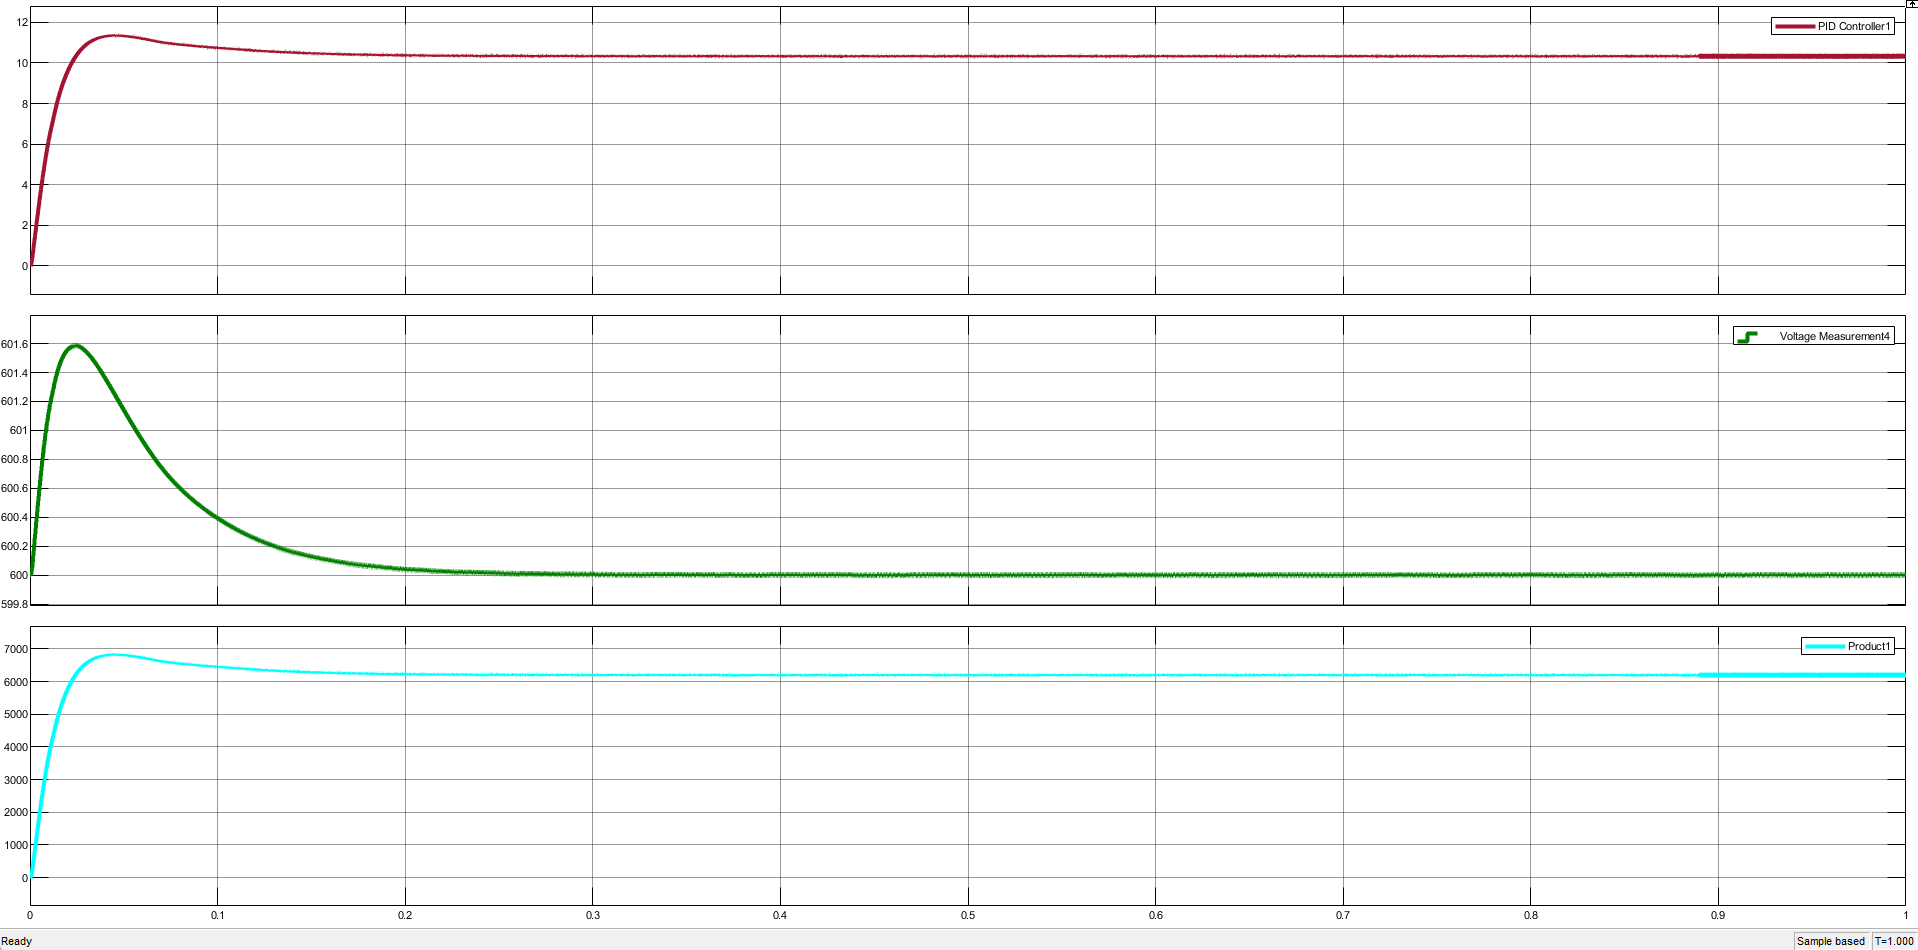
\includegraphics[width=1\textwidth]{Figures/5.1.40.png}
    \caption{Output current, voltage, power at 500 shading.}
    \label{fig:Output current, voltage, power at 500 shading}
\end{figure}

\subsubsection{Results of Simulation in Case of Shading (Ir = 250) at One Module at One String}
\noindent
\begin{minipage}[t]{0.5\textwidth}
\vspace{0pt}
\begin{itemize}
  \item As shown, the output power decreases as the current decreases only in the string that has shaded module, but the other string is unshaded, so it outputs the max power.
  \item As shown, the output power in string configuration is more than the output power in central configuration and this is the key difference between them and why is string is better in shading.
  \item Dc link voltage still maintained at 600\,V due to closed loop with PI.  

  \item Ripples of inductor current of string 1 $= 17.5 - 16.6 = 0.9$\,A.\
  \item Ripples of inductor current of string 2 $= 5.1 - 4.2 = 0.9$\,A.\
\end{itemize}
\end{minipage}
\hfill
\begin{minipage}[t]{0.3\textwidth}
\vspace{0pt}
  \centering
  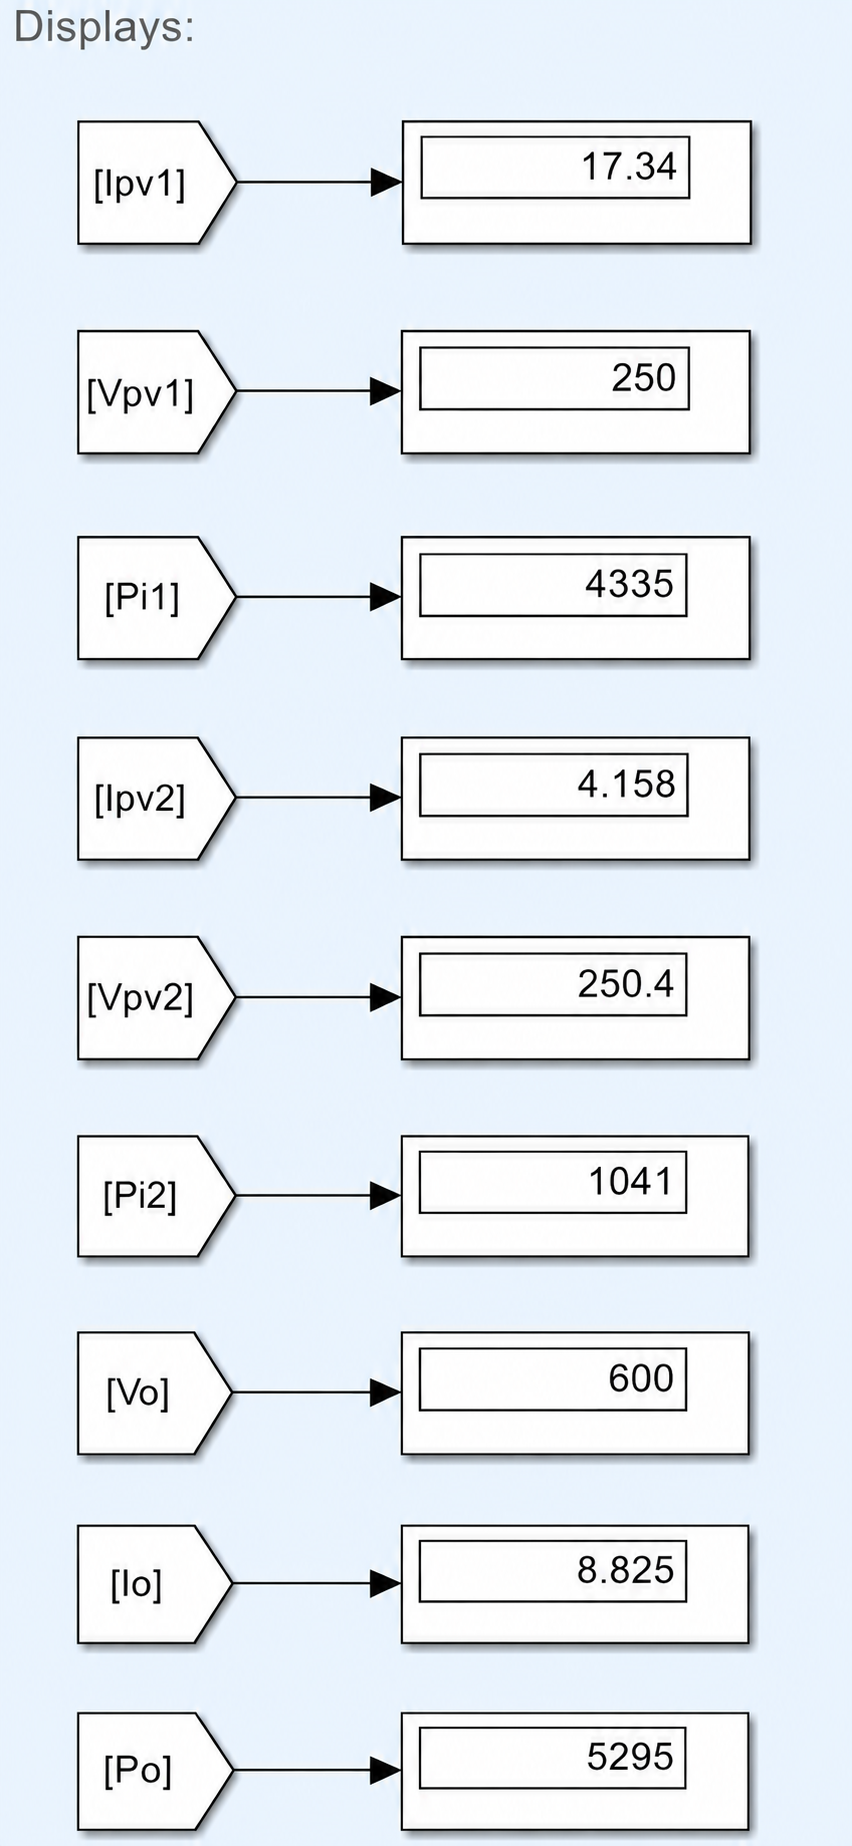
\includegraphics[width=\textwidth]{Figures/5.1.72.png}
  \captionof{figure}{Displays of string configuration at 250 shading.}
  \label{fig:Displays of string configuration at 250 shading}
\end{minipage}
\paragraph{Graphs}
\begin{figure}[H]
    \centering
    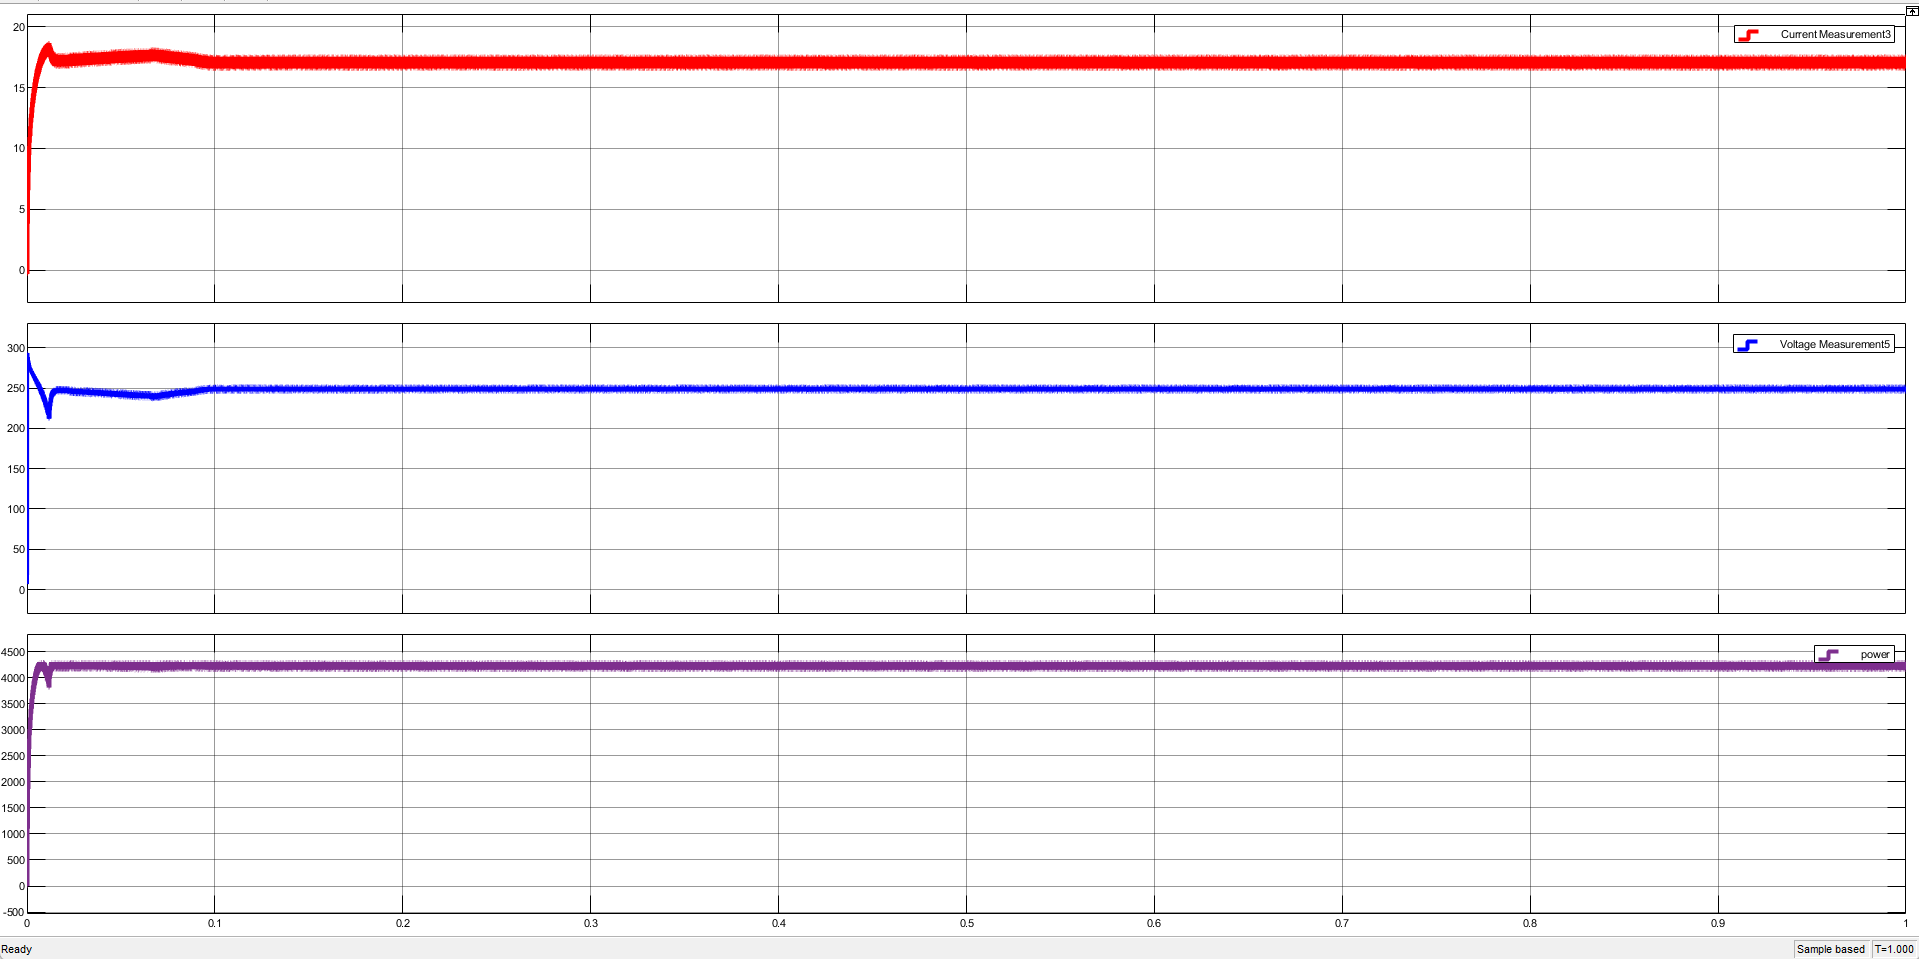
\includegraphics[width=1\textwidth]{Figures/5.1.42.png}
    \caption{Input current, voltage, power at string 1 at 250 shading.}
    \label{fig:input current, voltage, power at string 1 at 250 shading}
\end{figure}
\begin{figure}[H]
    \centering
    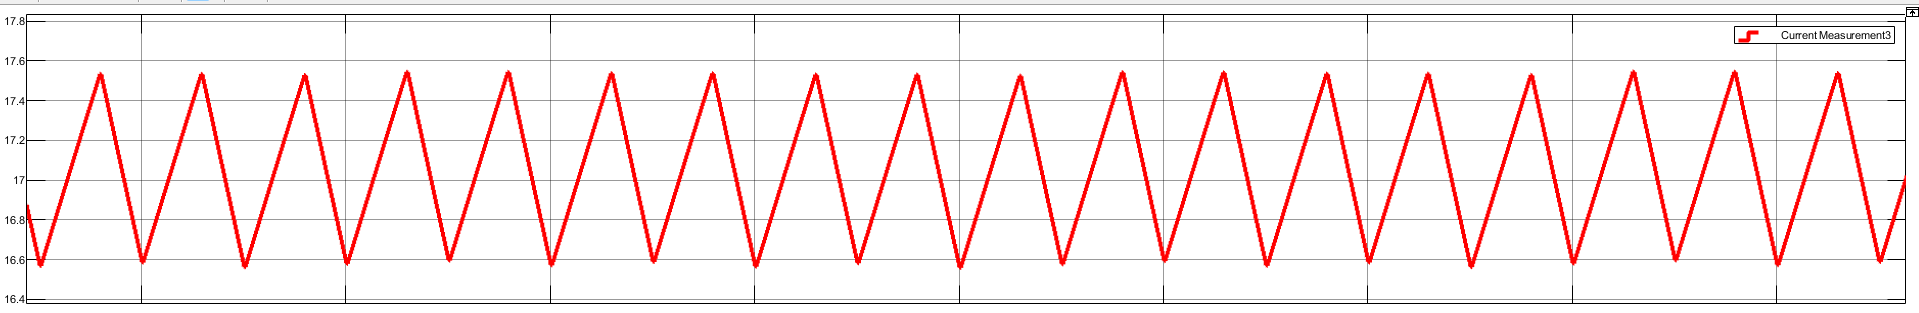
\includegraphics[width=1\textwidth]{Figures/5.1.43.png}
    \caption{Ripples of inductor current of string 1 at 250 shading.}
    \label{fig:ripples of inductor current of string 1 at 250 shading}
\end{figure}
\begin{figure}[H]
    \centering
    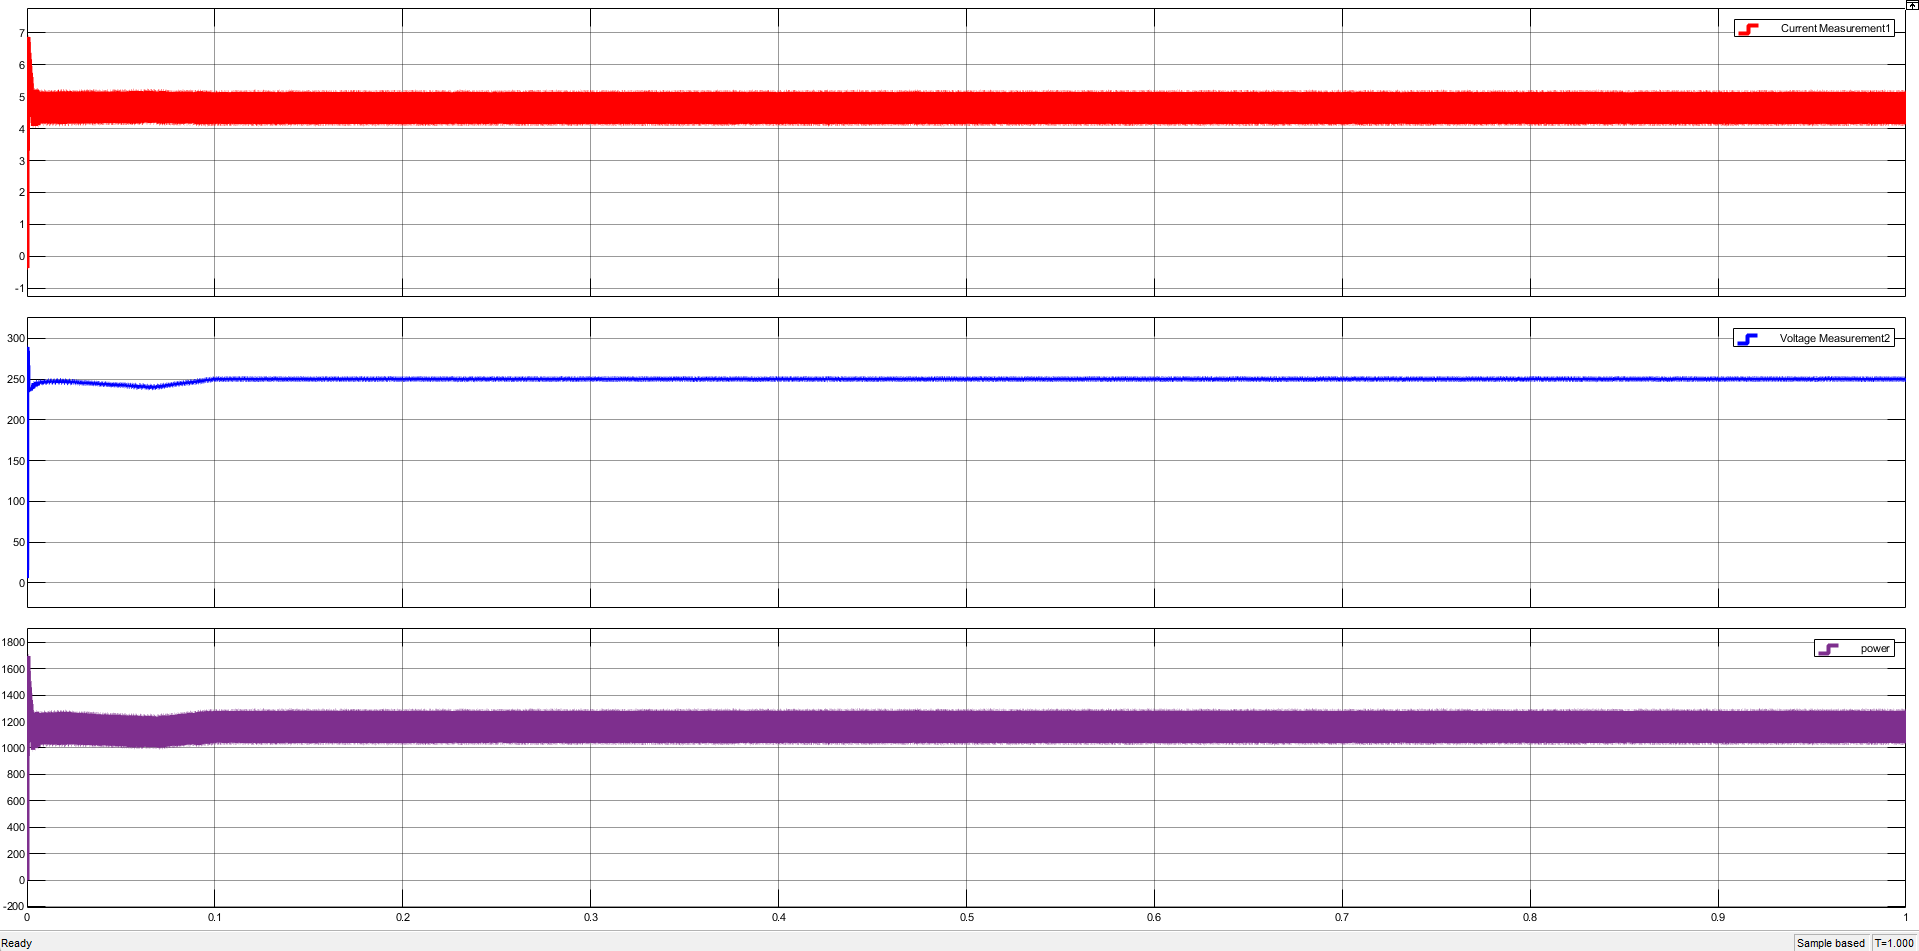
\includegraphics[width=0.9\textwidth]{Figures/5.1.44.png}
    \caption{Input current, voltage, power at string 2 at 250 shading.}
    \label{fig:input current, voltage, power at string 2 at 250 shading}
\end{figure}
\begin{figure}[H]
    \centering
    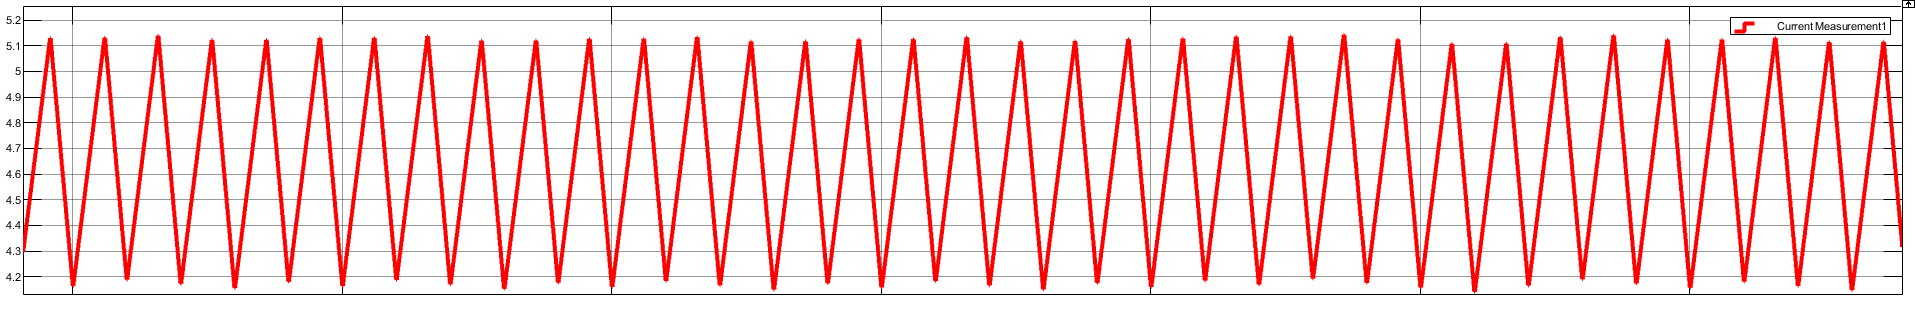
\includegraphics[width=1\textwidth]{Figures/5.1.45.png}
    \caption{Ripples of inductor current of string 2 at 250 shading.}
    \label{fig:ripples of inductor current of string 2 at 250 shading}
\end{figure}
\begin{figure}[H]
    \centering
    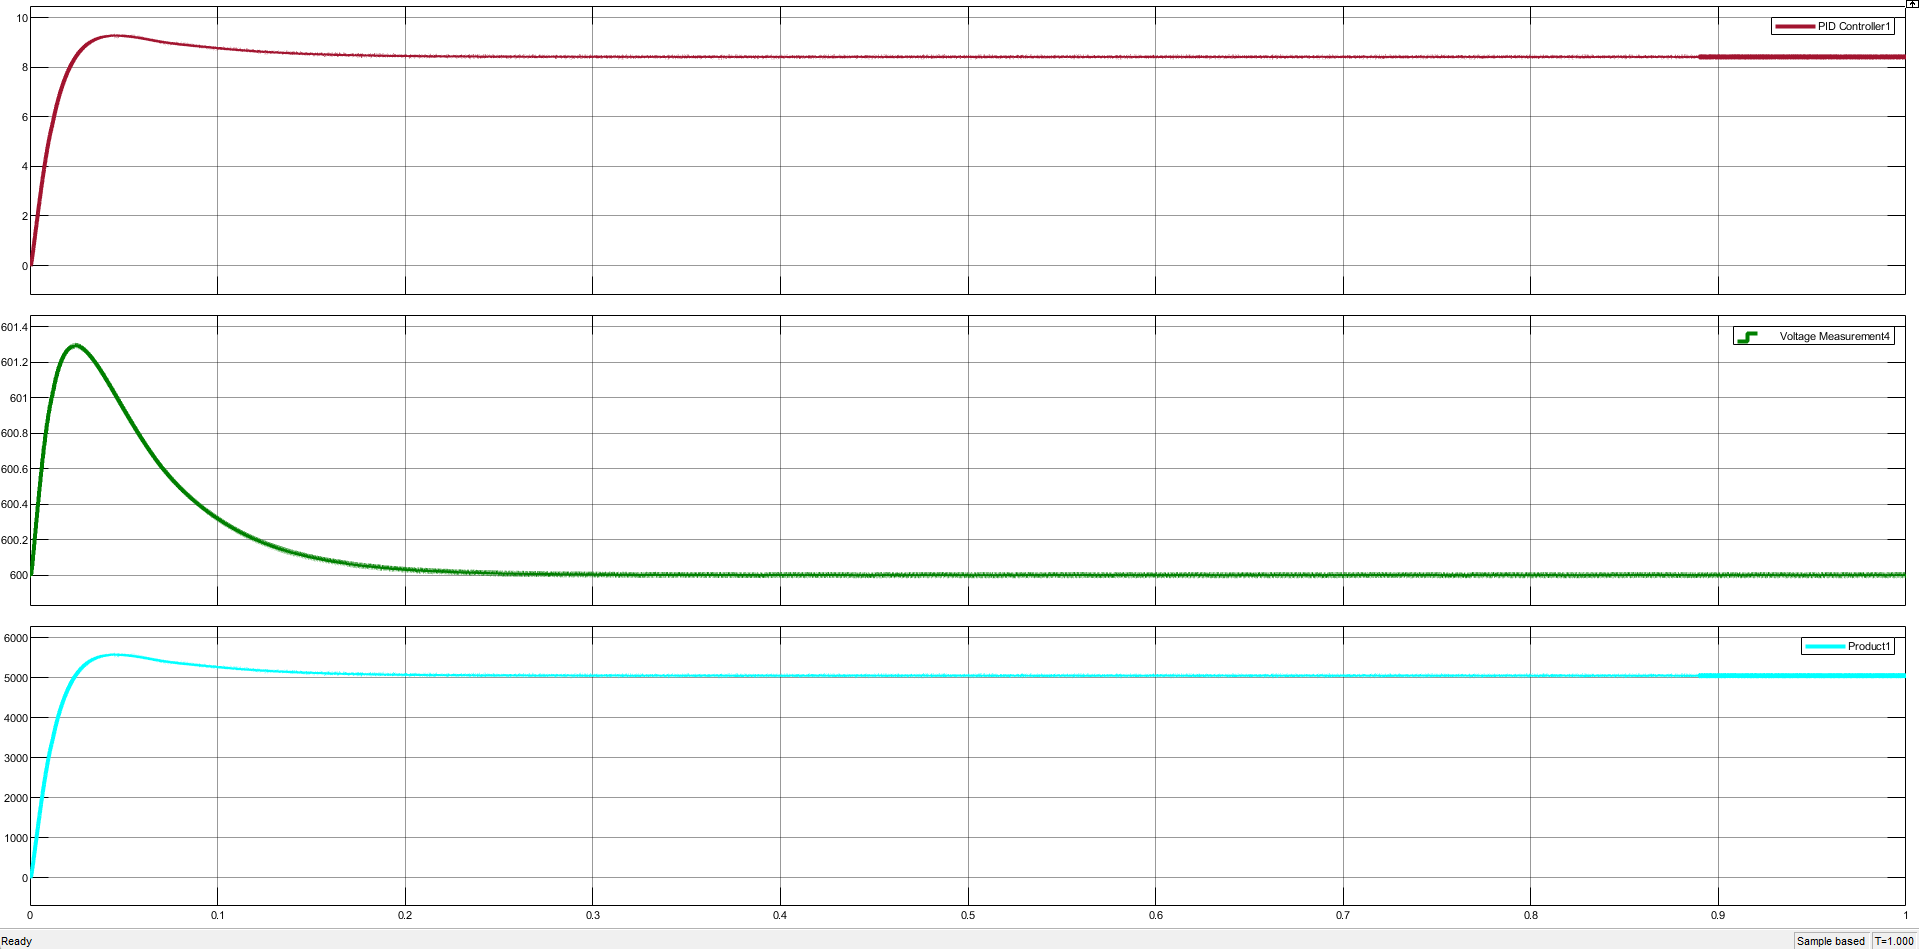
\includegraphics[width=0.9\textwidth]{Figures/5.1.46.png}
    \caption{Output current, voltage, power at 250 shading.}
    \label{fig:Output current, voltage, power at 250 shading}
\end{figure}

\subsection{Interleaved Central Configuration}
\subsubsection{Topology of Interleaved Boost Converter}
% ==========================================================
% SECTION 5.1.4: TWO-PHASE INTERLEAVED BOOST CONVERTER DESIGN
% ==========================================================

Conventional boost converters exhibit inherent performance limitations when deployed in high-power applications, primarily characterized by elevated input current ripple and increased thermal stress on switching devices. To mitigate these drawbacks and ensure optimal power extraction from the $8520\text{ W}$ photovoltaic (PV) array, a Two-Phase Interleaved Boost Converter (IBC) architecture was selected.

While a standard single-phase boost converter offers a lower component count, the interleaved configuration provides critical operational advantages for high-power integration across three primary domains:

\begin{enumerate}
    \item \textbf{Interleaving and Ripple Cancellation:} \\
    By implementing a $180^\circ$ spatial phase shift between the gate-drive control signals of the two parallel switching branches, the high-frequency inductor current ripples actively undergo destructive interference (cancellation). This interleaving mechanism yields a significantly smoother net input current waveform. Minimizing this current ripple prevents high-frequency voltage oscillations at the PV terminals, thereby enhancing the tracking precision and dynamic stability of the Global Maximum Power Point Tracking (GMPPT) algorithm.
    \newpage
    \item \textbf{Thermal Distribution via Current Sharing:} \\
    Under nominal peak operating conditions, the total array output current of $34.72\text{ A}$ is uniformly split between the two interleaved channels. Consequently, each discrete phase conducts an average current of only $17.36\text{ A}$. This reduction in localized current density scales down conduction losses ($I^2R$) and switching stresses across the power MOSFETs and diodes, minimizing thermal dissipation, improving reliability, and boosting the converter's net conversion efficiency.   
    \item \textbf{Volumetric and Filter Optimization:} \\
    The multi-phase interleaved operation effectively doubles the fundamental ripple frequency seen at the input and output filter stages ($f_{\text{ripple}} = 2f_s$). Because the required filter inductance and capacitance values are inversely proportional to the operating ripple frequency, this frequency doubling dramatically reduces the structural requirements for the passive components. As a result, the physical size, weight, magnetic core volume, and overall manufacturing cost of the power electronic interface are significantly minimized.
\end{enumerate}

\begin{figure}[H]
    \centering
    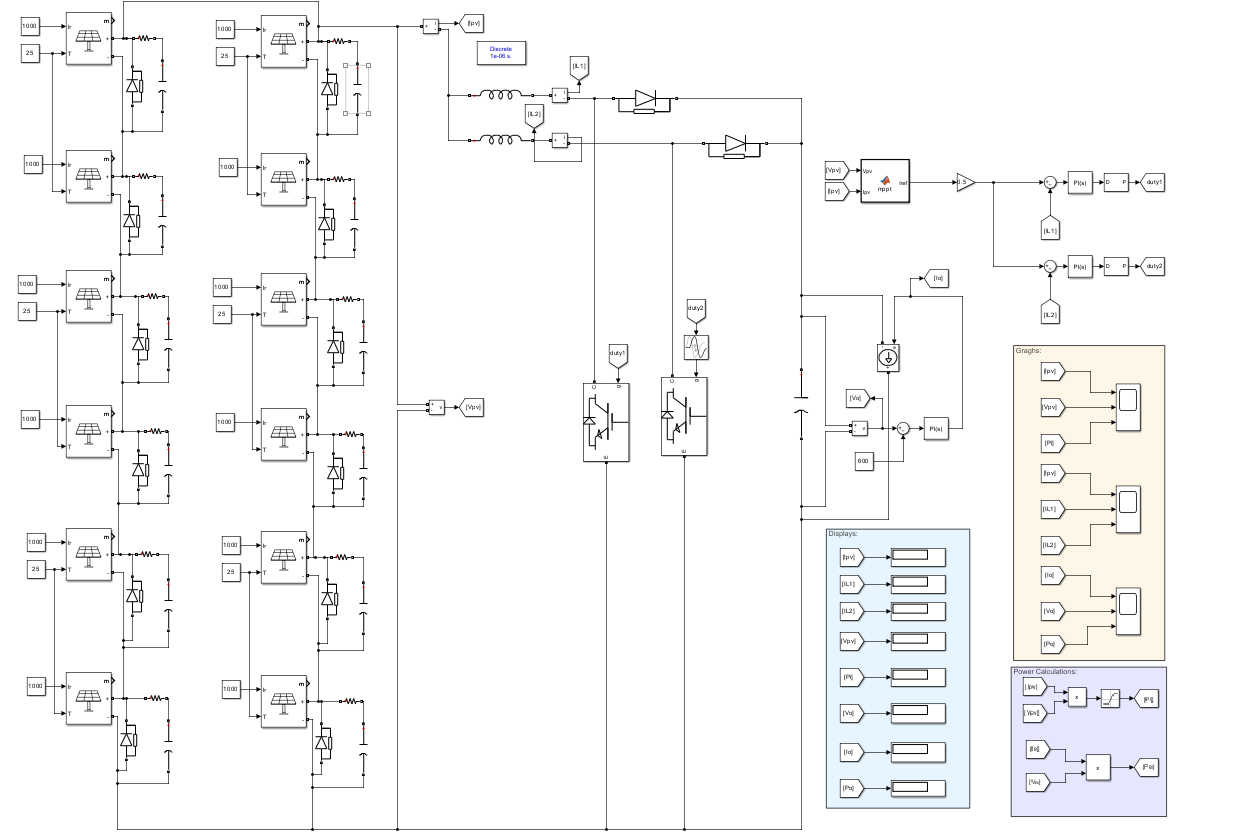
\includegraphics[width=1.1\textwidth]{Figures/5.1.47.png}
    \caption{ Interleaved central with load configuration.}
    \label{fig:interleaved central with load configuration}
\end{figure}

\subsubsection{Results of Simulation in Case of No Shading}
\noindent
\begin{minipage}[t]{0.5\textwidth}
\vspace{0pt}
\begin{itemize}
  \item The power display shows 8490\,W, which is nearly identical to the theoretical 8520\,W target. This confirms that the code is accurately tracking the Maximum Power Point.
  \item \textbf{DC-Link Stability:} The output voltage ($V_{DC}$) is maintained at
        exactly 600\,V. This proves that the DC-Link Voltage Control loop
        ($K_p = 8$, $K_i = 80$) and the Bulk Capacitor are effectively regulating the
        output despite the high-power flow.
   \item \textbf{Current sharing:} the inductor currents are almost equal and the input values of voltage and current align with the design calculation.      
  \item Ripples of inductor current $= 35.2 - 34.9 = 0.3$\,A.as seen ripples of current significantly decreases. 
\end{itemize}
\end{minipage}
\hfill
\begin{minipage}[t]{0.4\textwidth}
\vspace{0pt}
  \centering
  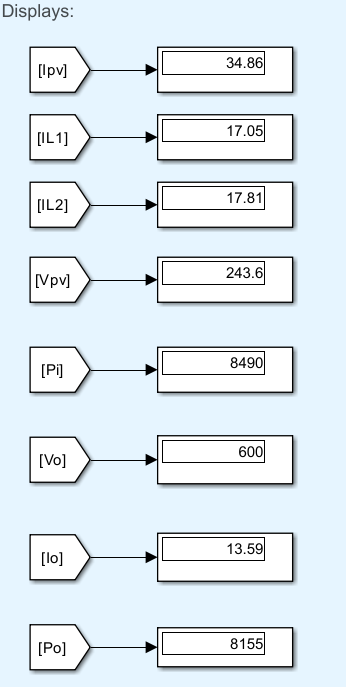
\includegraphics[width=\textwidth]{Figures/5.1.48.png}
  \captionof{figure}{Displays of interleaved central configuration.}
  \label{fig:displays of interleaved central configuration.}
\end{minipage}
\paragraph{Graphs}
\begin{figure}[H]
    \centering
    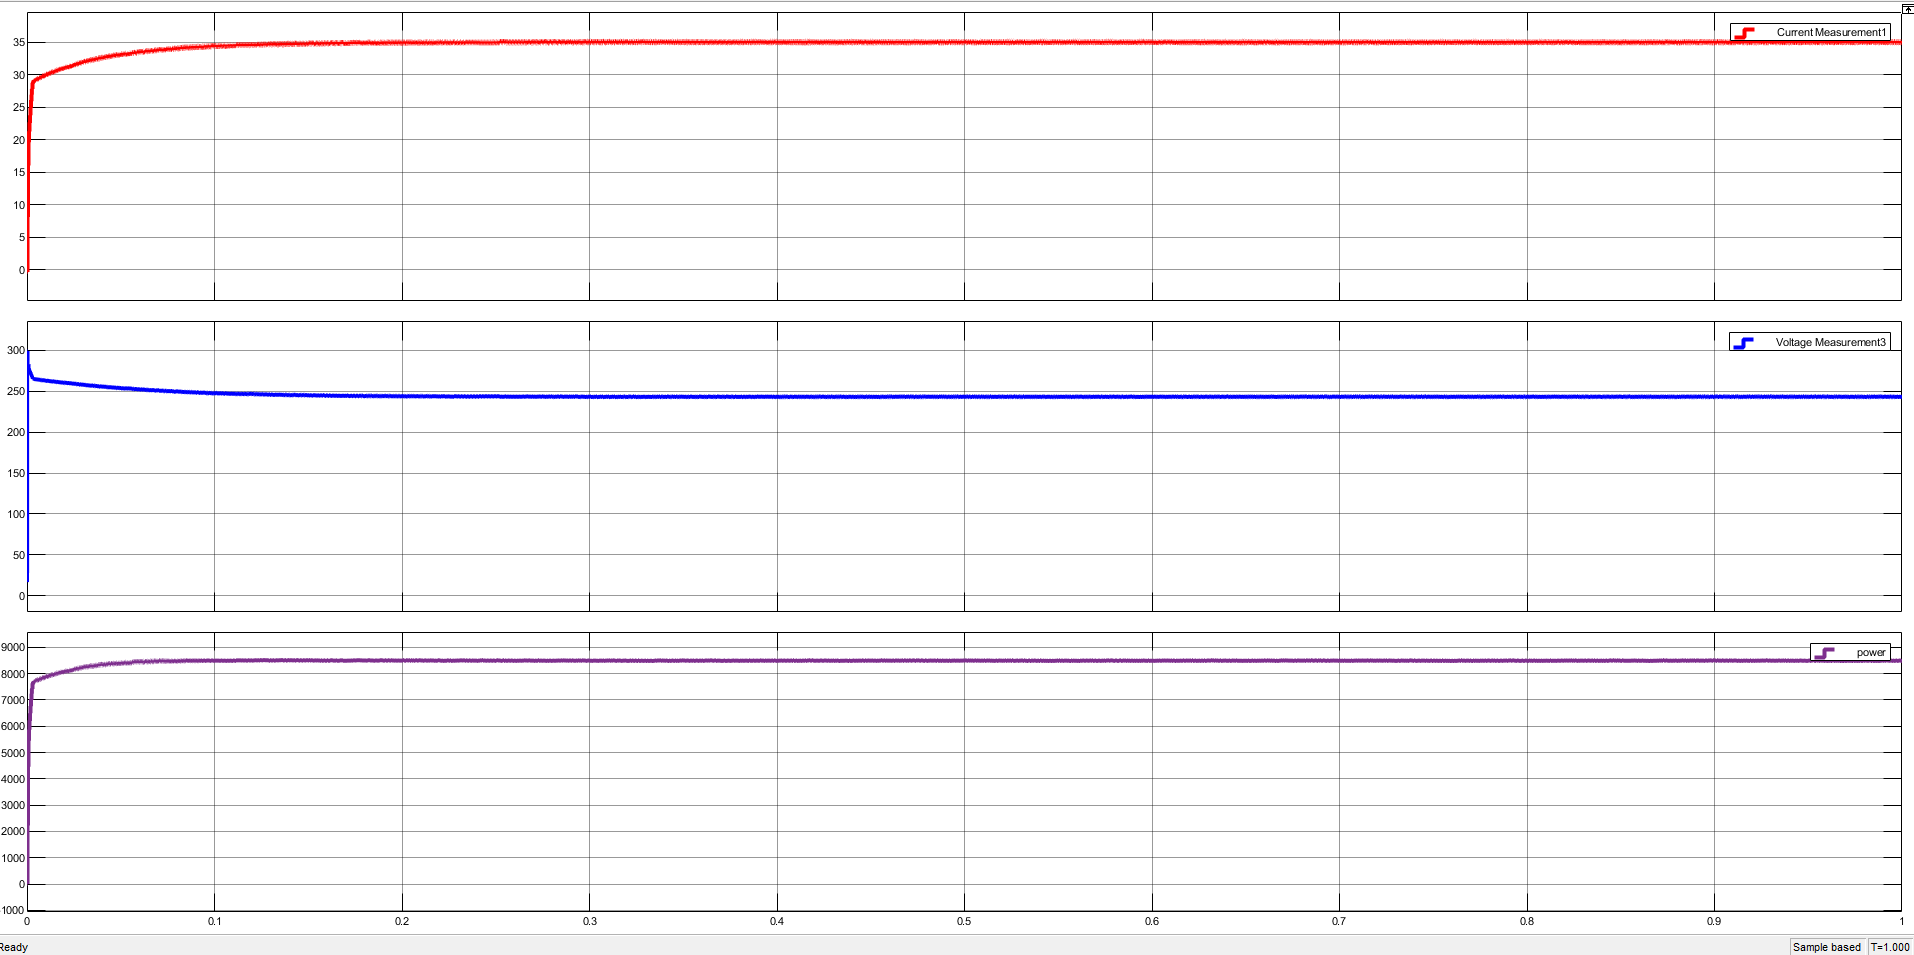
\includegraphics[width=0.9\textwidth]{Figures/5.1.49.png}
    \caption{Input current, voltage, power of interleaved central.}
    \label{fig:input current, voltage, power at no shading at interleaved central}
\end{figure}
\begin{figure}[H]
    \centering
    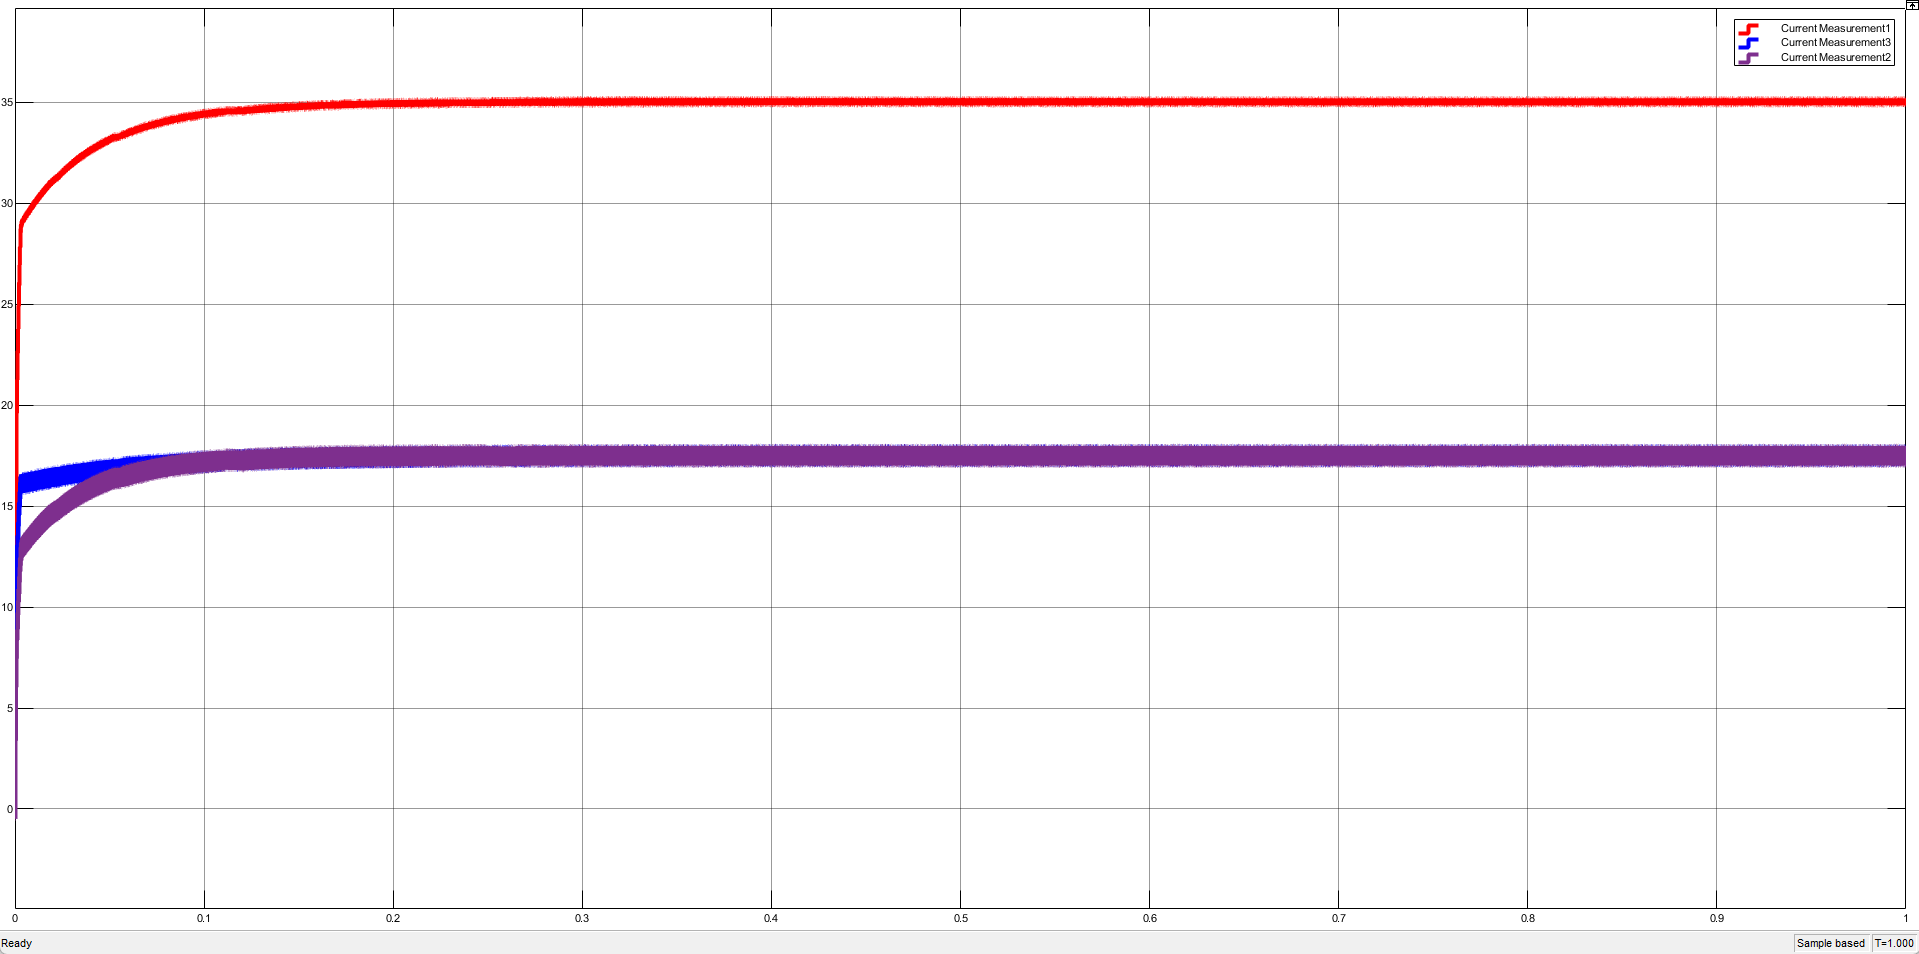
\includegraphics[width=0.9\textwidth]{Figures/5.1.50.png}
    \caption{Input total current, inductor current 1, inductor current 2.}
    \label{fig:input total current, inductor current 1, inductor current 2 at no shading at interleaved central}
\end{figure}
\begin{figure}[H]
    \centering
    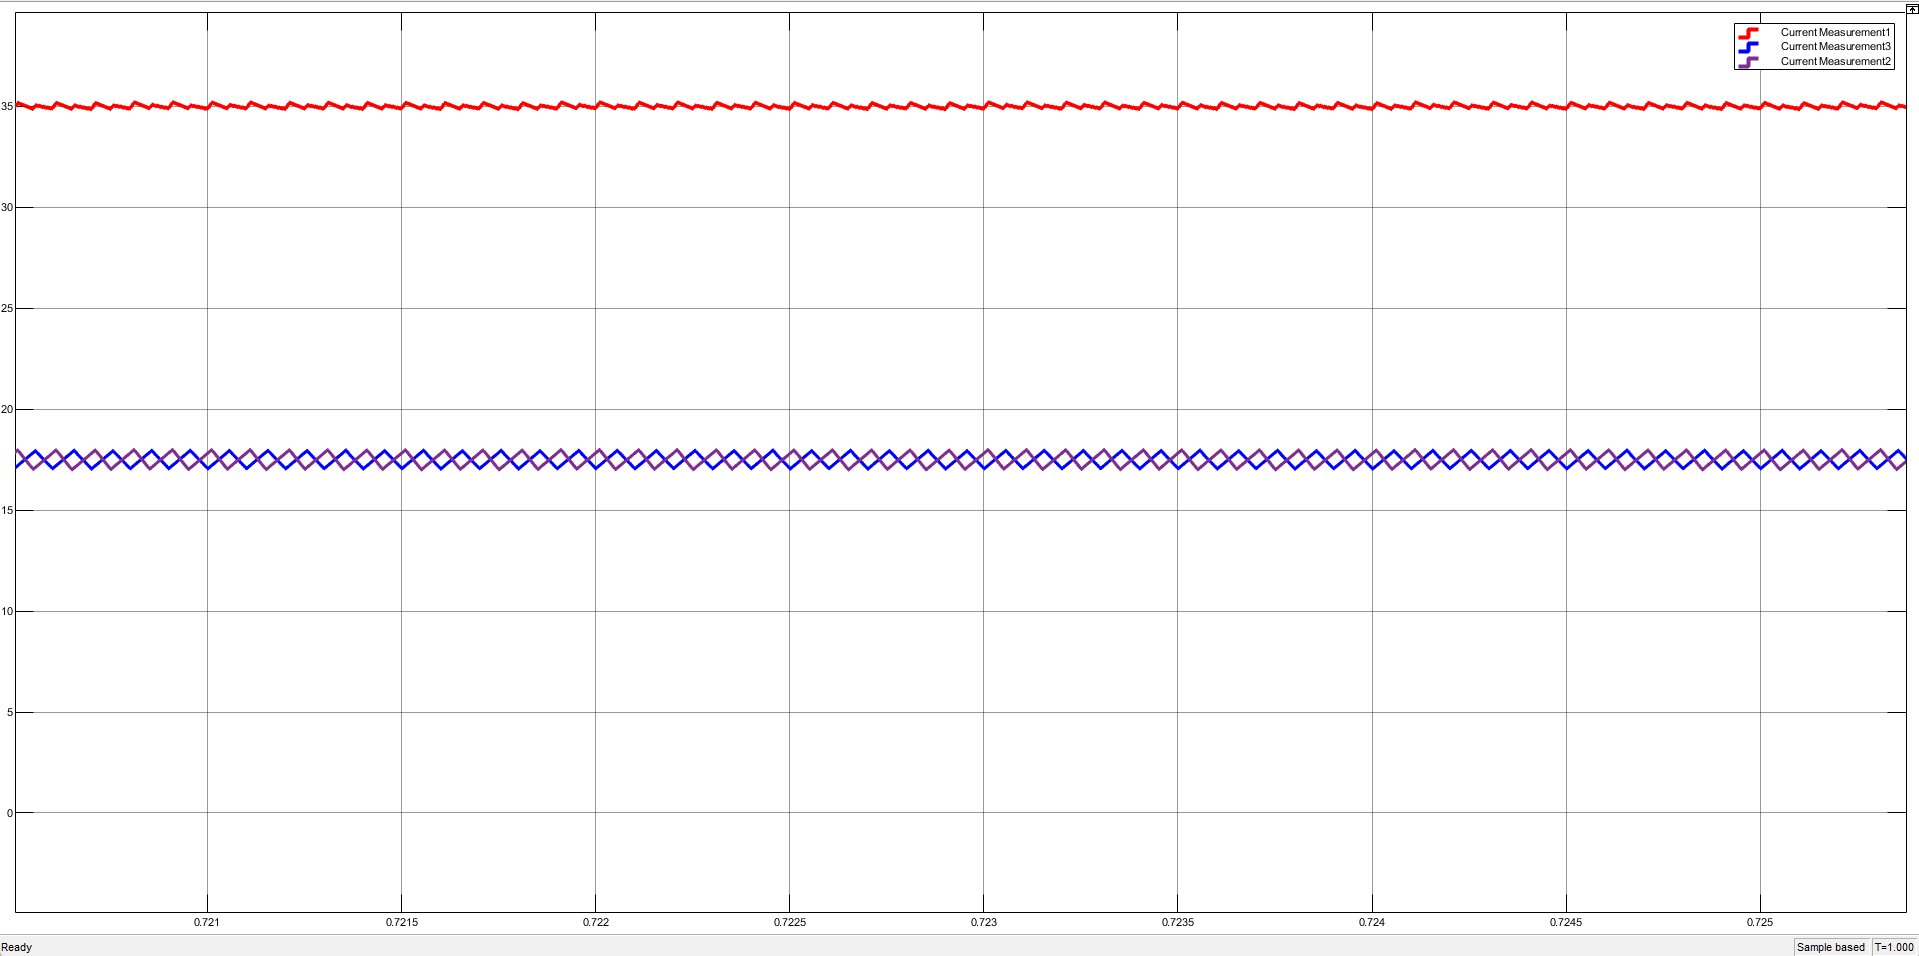
\includegraphics[width=0.9\textwidth]{Figures/5.1.51.png}
    \caption{Input total current, inductor current 1, inductor current 2.}
    \label{fig:input total current, inductor current 1, inductor current 2 zoom at no shading at interleaved central}
\end{figure}
\begin{figure}[H]
    \centering
    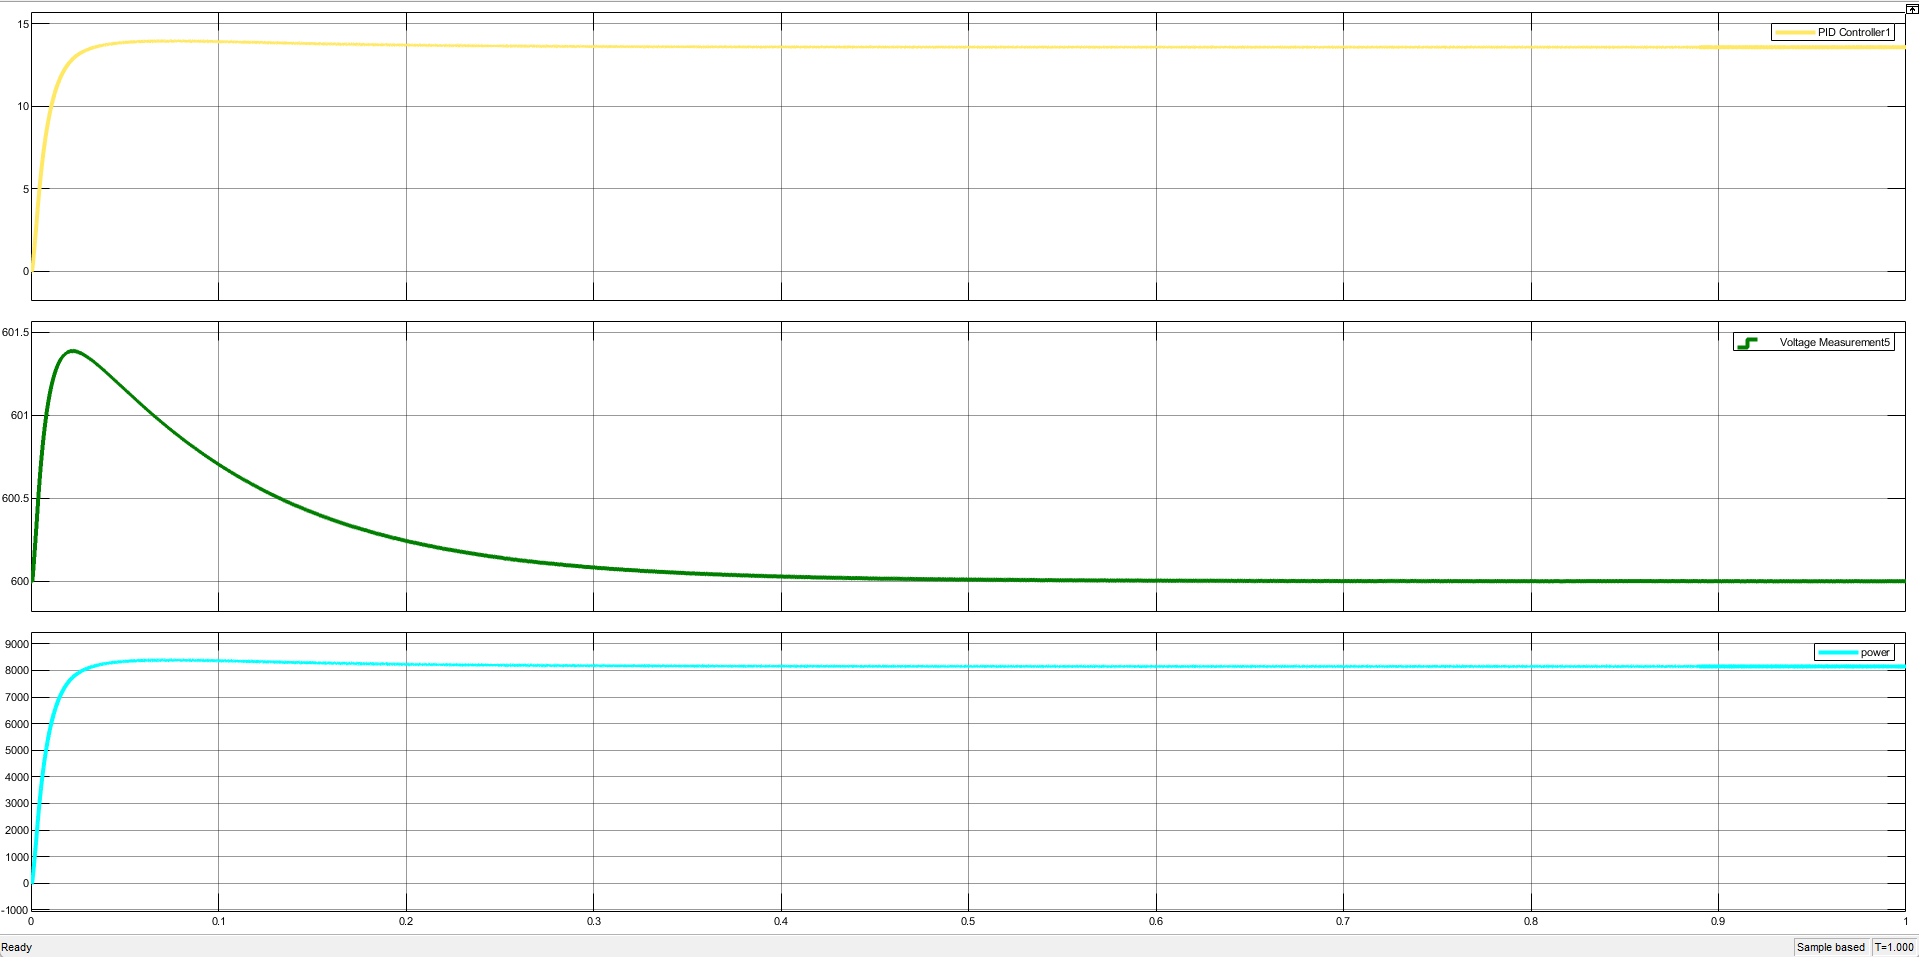
\includegraphics[width=0.9\textwidth]{Figures/5.1.52.png}
    \caption{Output current, voltage, power of interleaved central.}
    \label{fig:output current, voltage, power at no shading at interleaved central}
\end{figure}


\subsection{String Interleaved Configuration}
\begin{figure}[H]
    \centering
    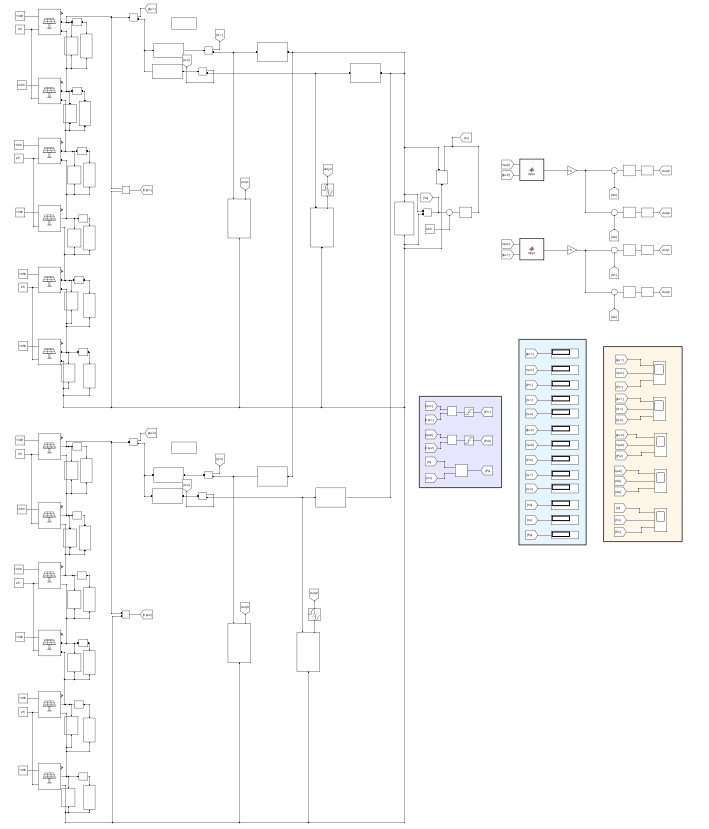
\includegraphics[width=1\textwidth]{Figures/5.1.53.png}
    \caption{ Interleaved string with load configuration.}
    \label{fig:interleaved string with load configuration}
\end{figure}
\subsubsection{Results of Simulation in Case of No Shading}
\noindent
\begin{minipage}[t]{0.5\textwidth}
\vspace{0pt}
\begin{itemize}
  \item Each string has its own interleaved boost converter with common dc link, so each string has its own MPPT and both tracks correctly max power.
  \item \textbf DC-Link  is maintained at exactly 600\,V due to PI closed loop control ($K_p = 5$, $K_i = 150$)
   \item \textbf{Current sharing:} the inductor currents are almost equal and the input values of voltage and current align with the design calculation.      
  \item Ripples of total inductor current of string 1 $= 35.2 - 34.9 = 0.3$\,A.as seen ripples of current significantly decreases. 
  \item Ripples of total inductor current of string 1 $= 35.2 - 34.9 = 0.3$\,A.as seen ripples of current significantly decreases.
\end{itemize}
\end{minipage}
\hfill
\begin{minipage}[t]{0.4\textwidth}
\vspace{0pt}
  \centering
  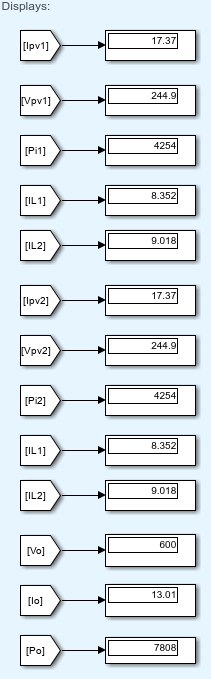
\includegraphics[width=\textwidth]{Figures/5.1.54.png}
  \captionof{figure}{Displays of interleaved string configuration..}
  \label{fig:Displays of interleaved string configuration.}
\end{minipage}

\begin{figure}[H]
    \centering
    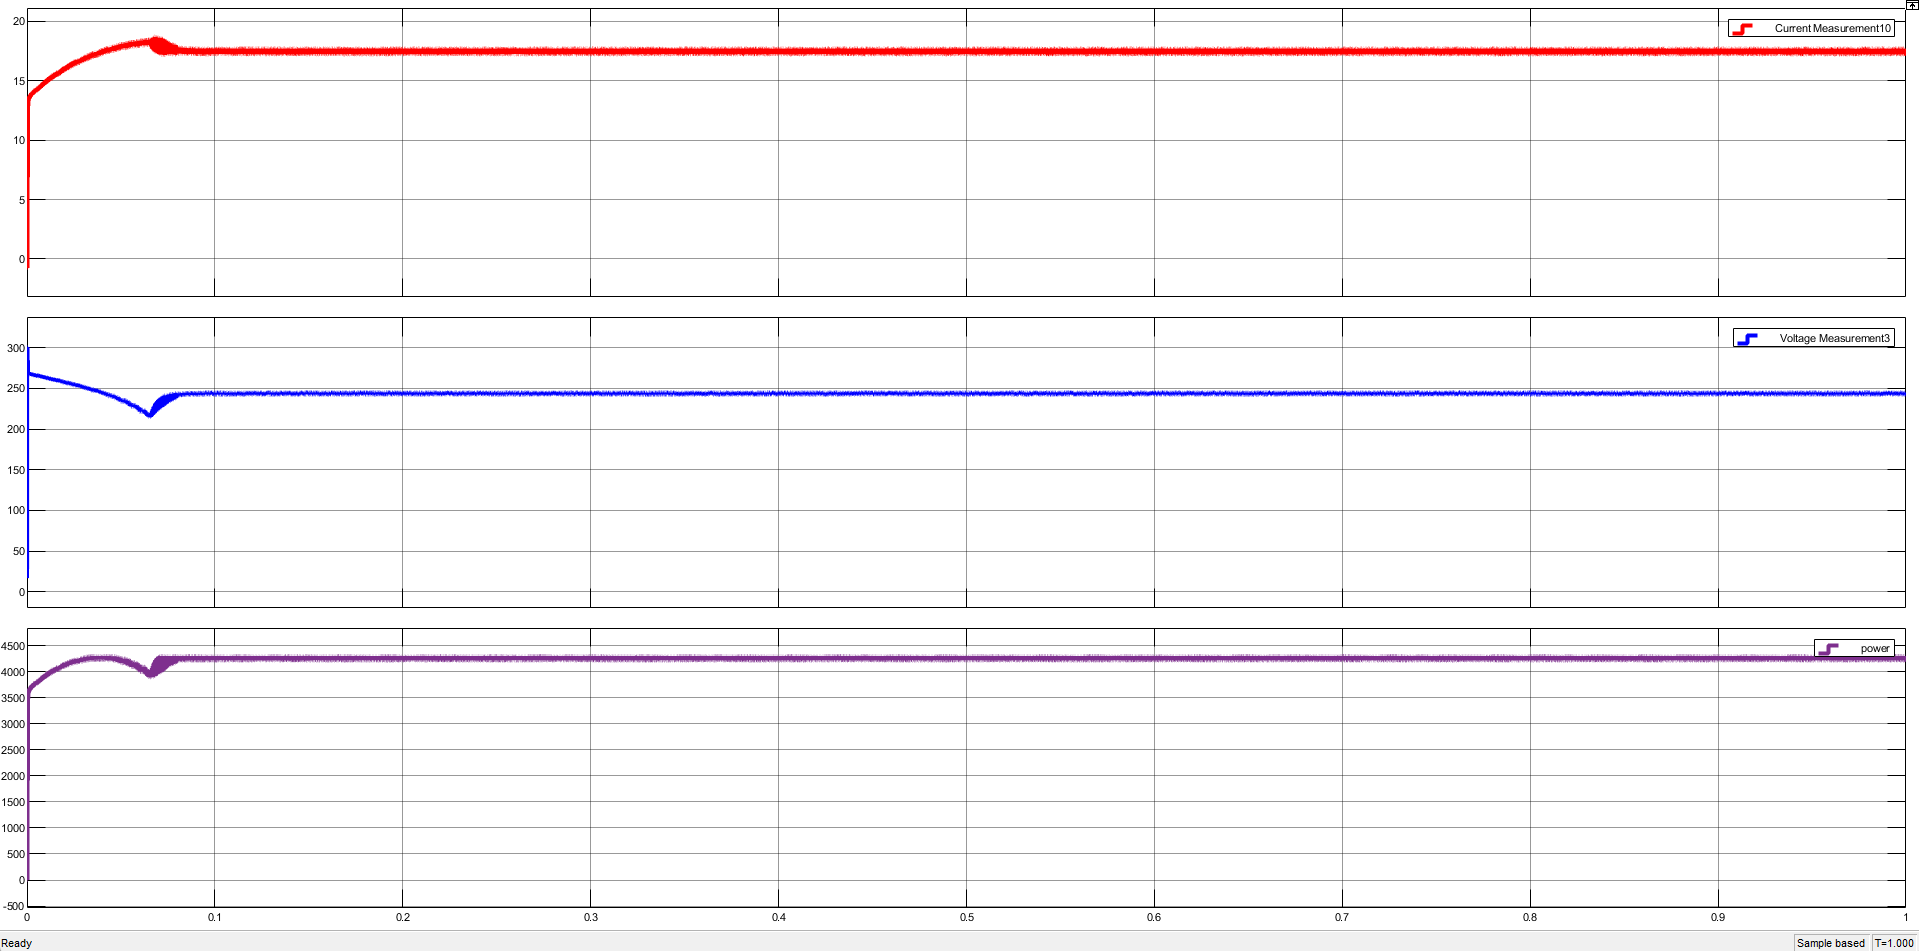
\includegraphics[width=0.9\textwidth]{Figures/5.1.55.png}
    \caption{Input current, voltage, power at string 1 of interleaved string.}
    \label{fig:input current, voltage, power at no shading at interleaved string at string 1}
\end{figure}
\begin{figure}[H]
    \centering
    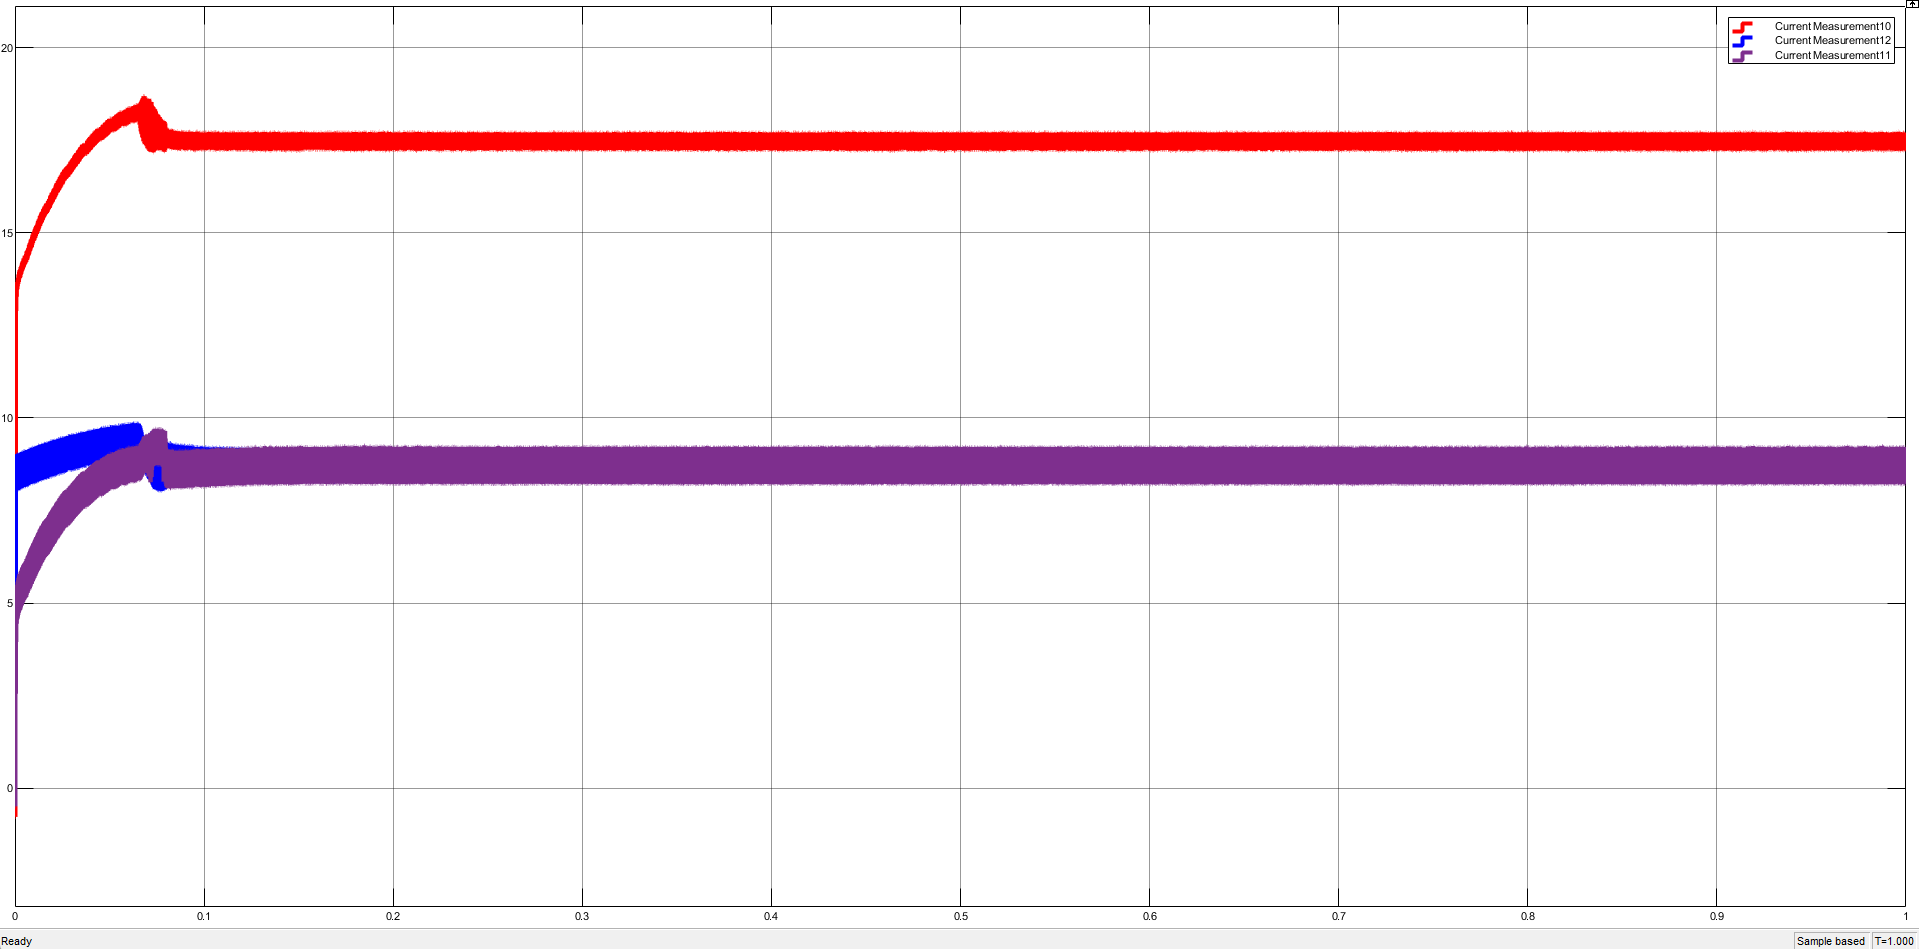
\includegraphics[width=0.9\textwidth]{Figures/5.1.56.png}
    \caption{Input total current, inductor current 1, inductor current 2 at string 1.}
    \label{fig:input total current, inductor current 1, inductor current 2 at no shading at interleaved string at string 1}
\end{figure}
\begin{figure}[H]
    \centering
    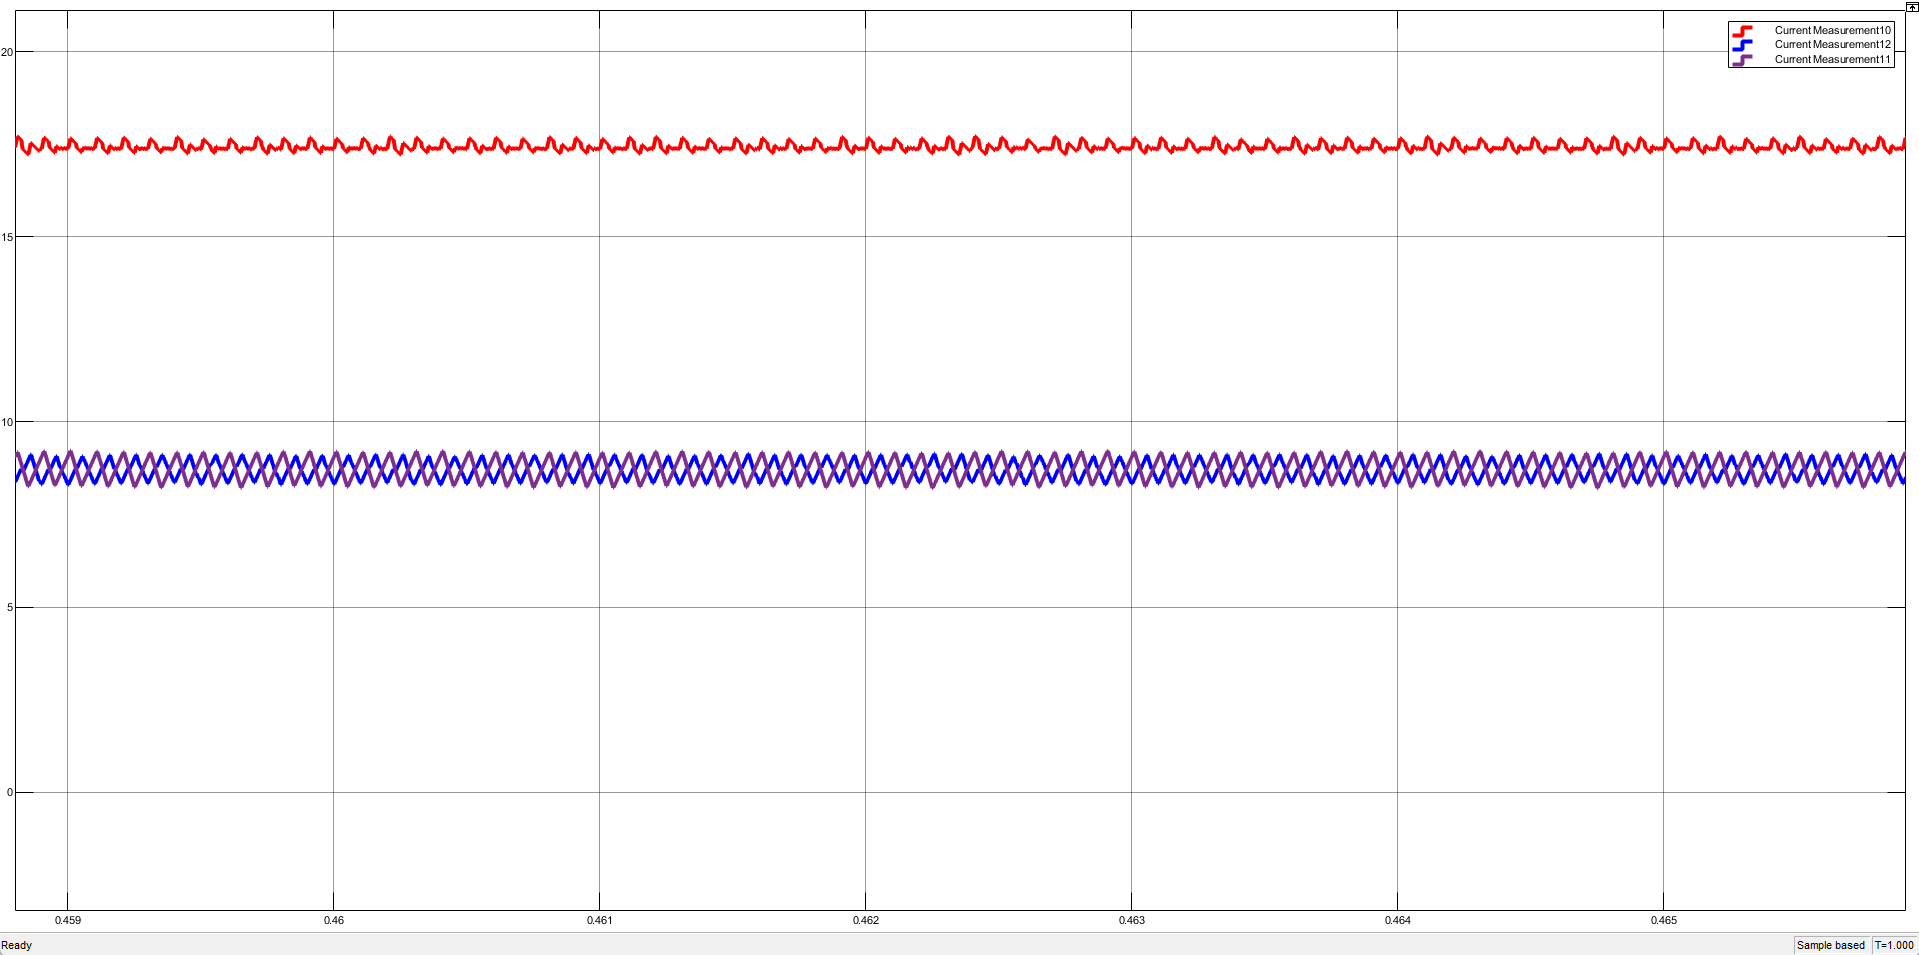
\includegraphics[width=0.9\textwidth]{Figures/5.1.57.png}
    \caption{Input total current, inductor current 1, inductor current 2 at string 1.}
    \label{fig:input total current, inductor current 1, inductor current 2 zoom at no shading at interleaved string at string 1}
\end{figure}
\begin{figure}[H]
    \centering
    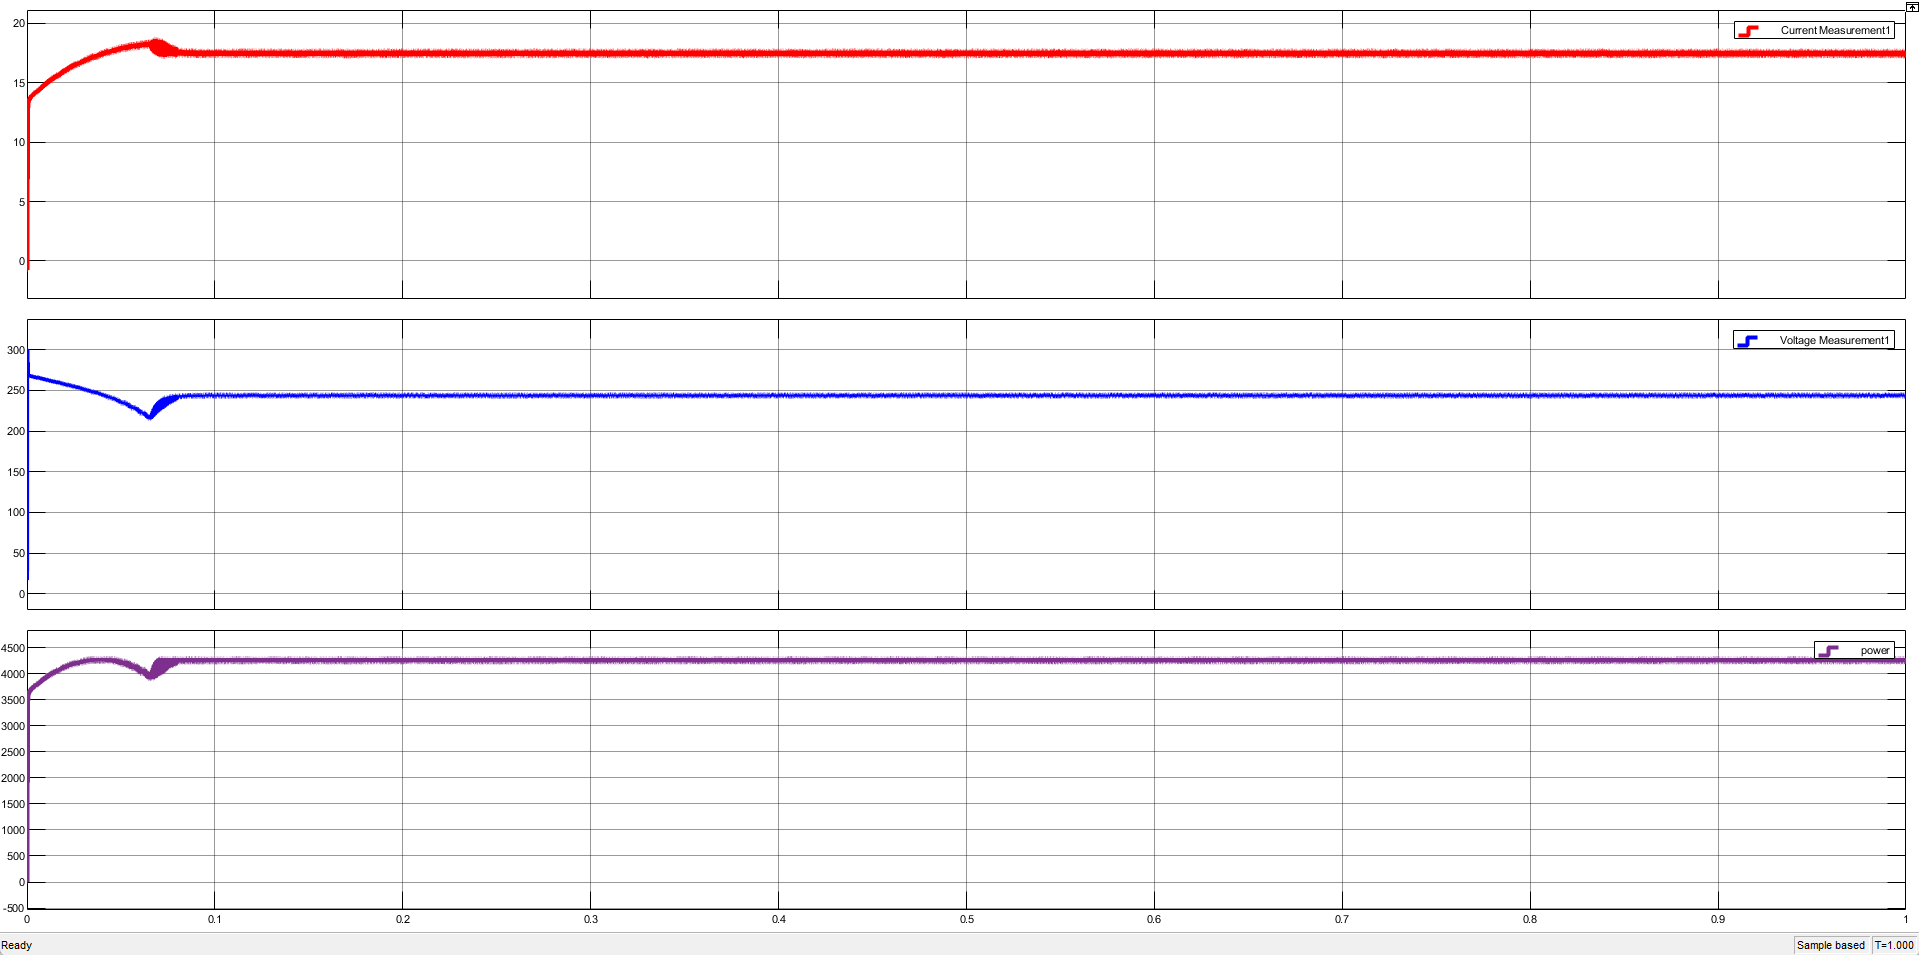
\includegraphics[width=0.9\textwidth]{Figures/5.1.58.png}
    \caption{Input current, voltage, power at string 2 of interleaved string.}
    \label{fig:input current, voltage, power at no shading at interleaved string at string 2}
\end{figure}
\begin{figure}[H]
    \centering
    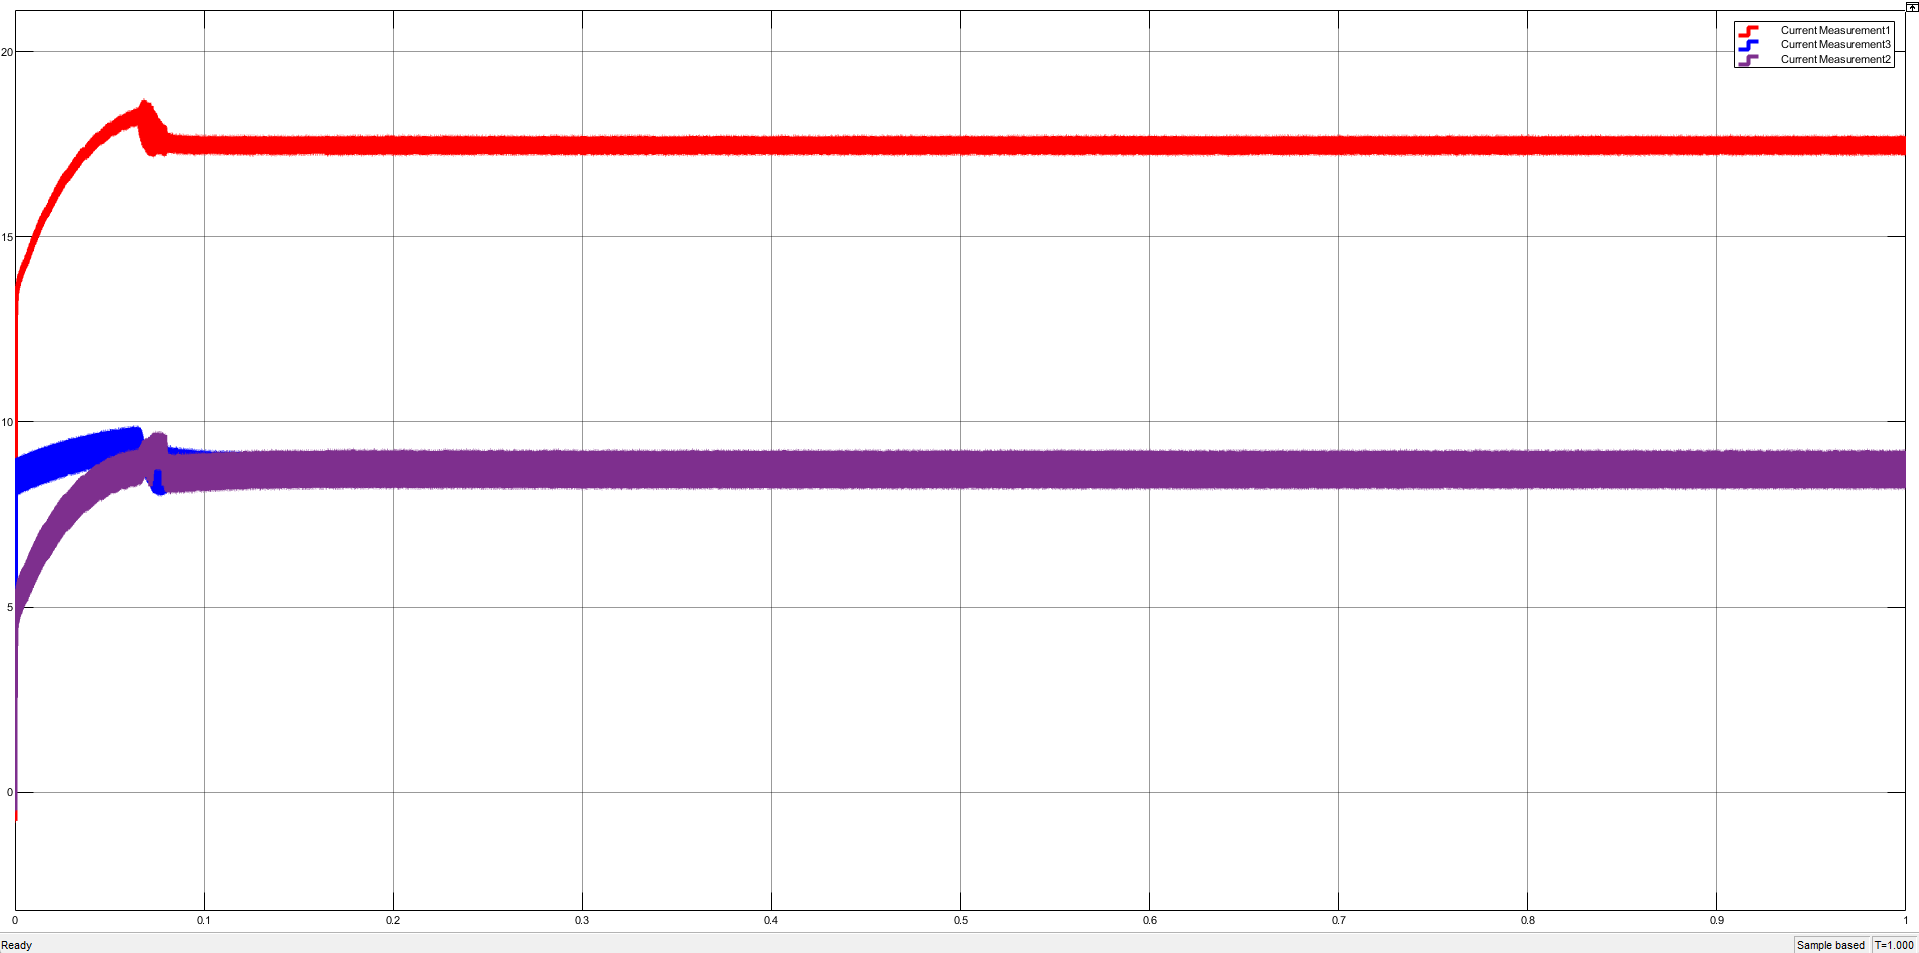
\includegraphics[width=0.9\textwidth]{Figures/5.1.59.png}
    \caption{Input total current, inductor current 1, inductor current 2 at string 2.}
    \label{fig:input total current, inductor current 1, inductor current 2 at no shading at interleaved string at string 2}
\end{figure}
\begin{figure}[H]
    \centering
    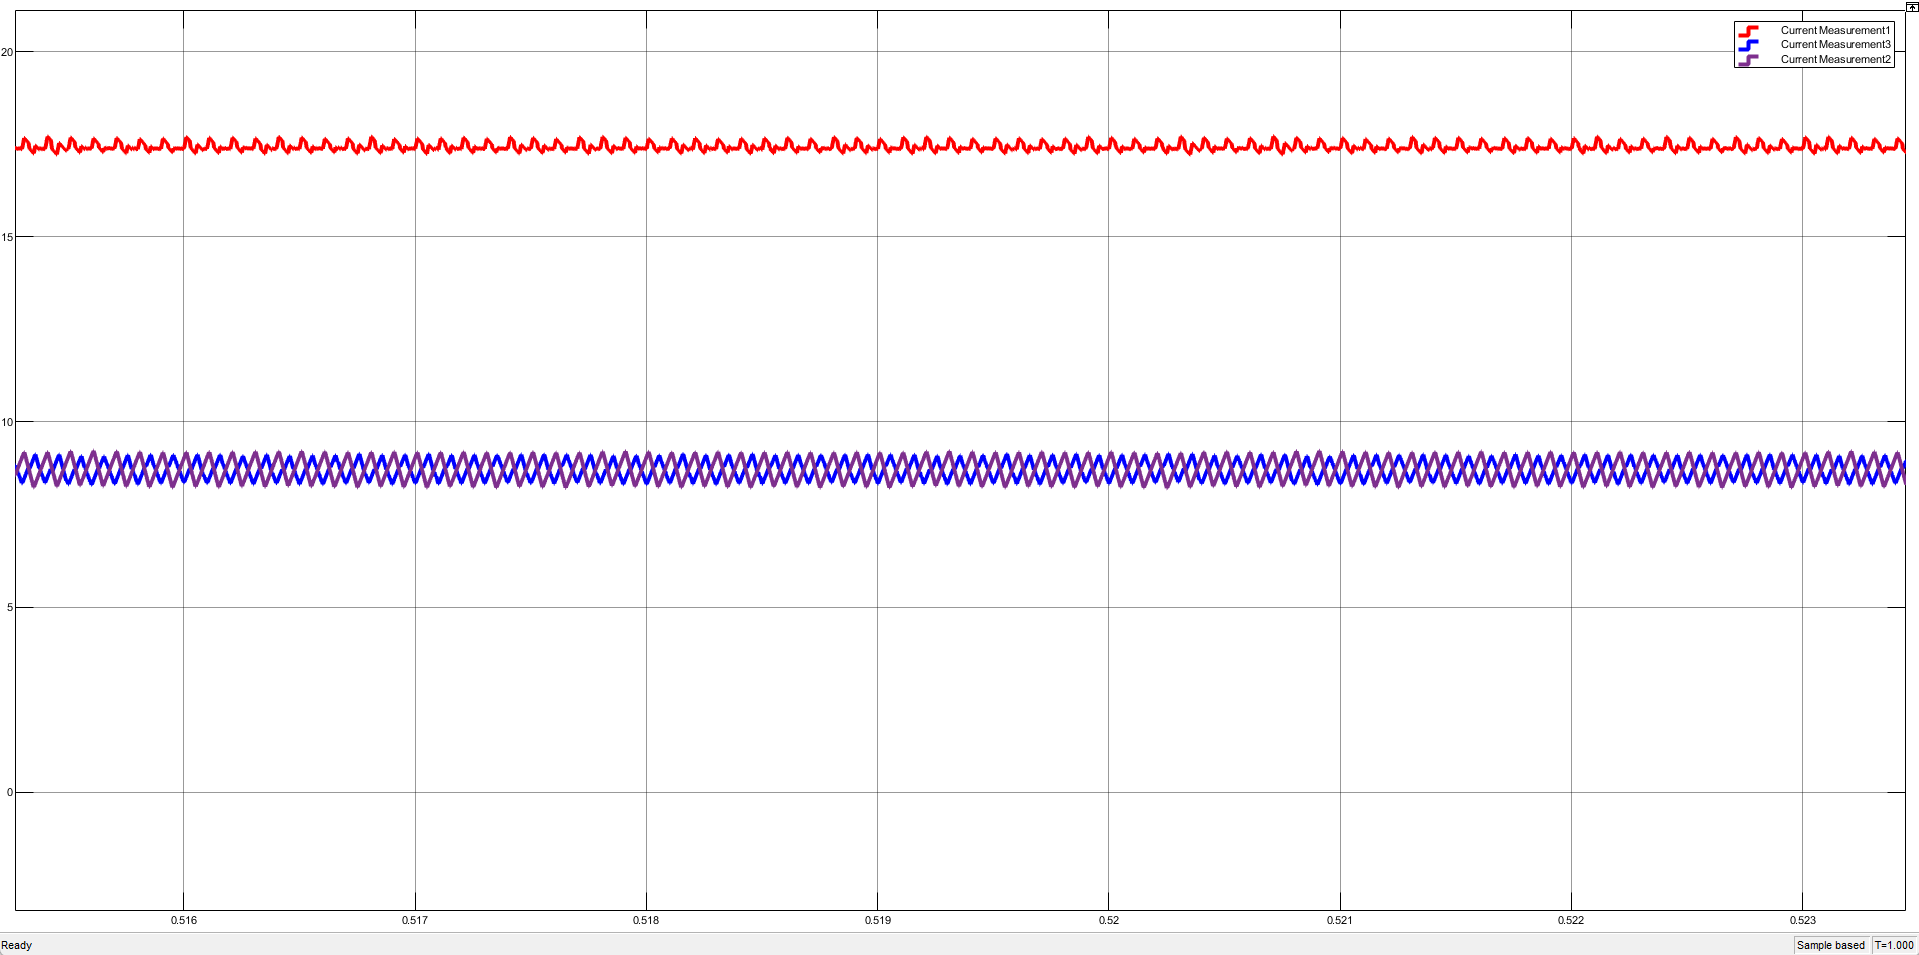
\includegraphics[width=0.9\textwidth]{Figures/5.1.60.png}
    \caption{Input total current, inductor current 1, inductor current 2 at string 2.}
    \label{fig:input total current, inductor current 1, inductor current 2 zoom at no shading at interleaved string at string 2}
\end{figure}
\begin{figure}[H]
    \centering
    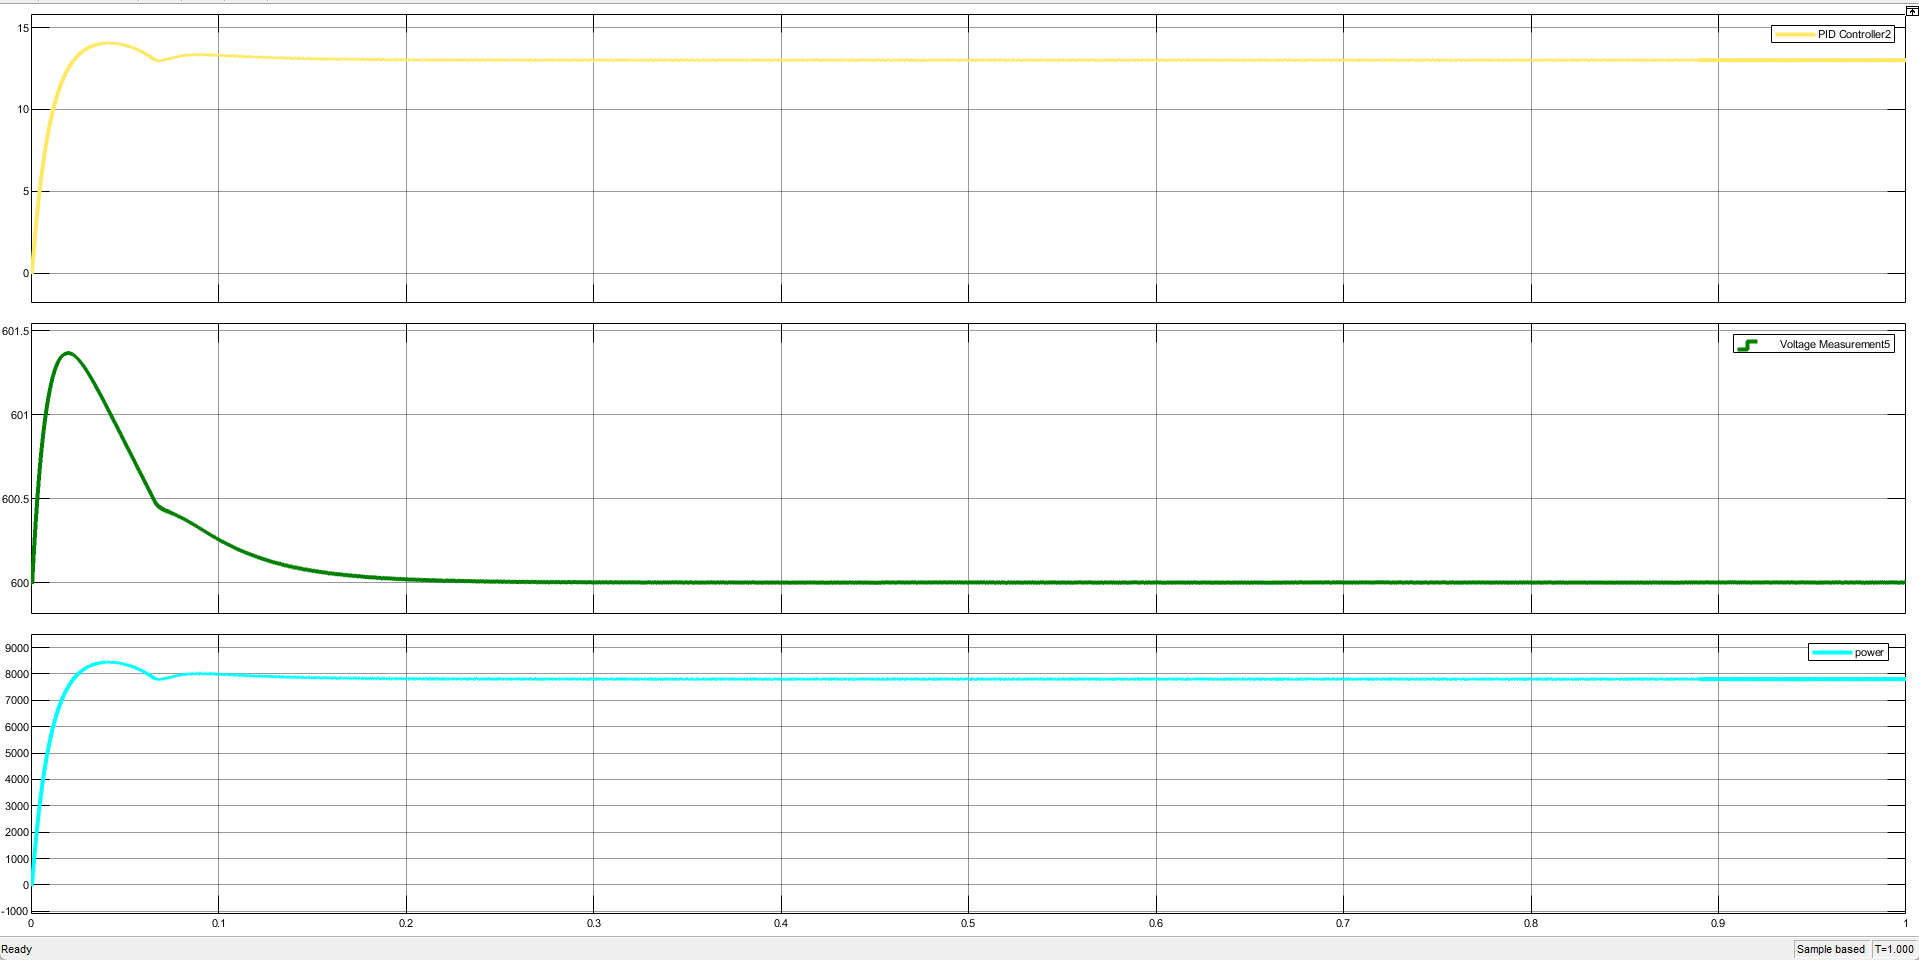
\includegraphics[width=0.9\textwidth]{Figures/5.1.61.png}
    \caption{Output current, voltage, power of interleaved string.}
    \label{fig:output current, voltage, power at no shading at interleaved string}
\end{figure}